%  Thesis for Xiaolei Chen

\documentclass[12pt]{report}
\usepackage{thesis}
\usepackage{graphicx}
\usepackage{amsmath}
\usepackage{amssymb}		% to see postscript files
\usepackage{doublespace}

\usepackage[dvips]{epsfig}
\usepackage{multirow}
\usepackage{color}
\usepackage{listings}
\usepackage{verbatim}
\usepackage{epstopdf}
\usepackage{subcaption}
\usepackage{mathrsfs}
\DeclareGraphicsExtensions{.pdf,.png,.jpg,.eps}

\def\doublespace{1.66}		% 1.66 for double spacing with 12pt
\def\singlespace{1.00}		% 1.00 for single spacing
\def\defaultspace{\doublespace}	% adjust spacing factor

%
% Color
%
\definecolor{codegreen}{rgb}{0,0.6,0}
\definecolor{codegray}{rgb}{0.5,0.5,0.5}
\definecolor{codepurple}{rgb}{0.58,0,0.82}
\definecolor{backcolour}{rgb}{0.95,0.95,0.92}

\lstdefinestyle{mystyle}{
    backgroundcolor=\color{backcolour},
    commentstyle=\color{codegreen},
    keywordstyle=\color{magenta},
    numberstyle=\tiny\color{codegray},
    stringstyle=\color{codepurple},
    basicstyle=\footnotesize,
    breakatwhitespace=false,
    breaklines=true,
    captionpos=b,
    keepspaces=true,
    numbers=left,
    numbersep=5pt,
    showspaces=false,
    showstringspaces=false,
    showtabs=true,
    tabsize=2,
    frame=\shadowbox
}
\lstset{style=mystyle}
				

%\newcommand{\RR}{\mathcal{R}}
\newcommand{\posdisc}{\delta}
\newcommand{\widebar}[1]{\bar{#1}}
\newcommand{\skspd}{s}
\newcommand{\RR}{\mathrm{I\!R\!}}

\newcommand{\rarefset}{\mathcal{R}}
\newcommand{\shockset}{\mathcal{S}}
\newcommand{\waveset}{\mathcal{W}}
\newcommand{\Lstar}{\mathcal{L}^*}
\newcommand{\Leps}{\mathcal{L}_{\epsilon}}
\newcommand{\fan}{\mathcal{F}}
\newcommand{\lls}{l^*}
\newcommand{\lle}{l}
\newcommand{\gm}{\gamma}
\newcommand{\al}{\alpha}
\newcommand{\lbd}{\lambda}
\newcommand{\bt}{\beta}
\newcommand{\zt}{\zeta}
\newcommand{\fal}[2]{\{ \alpha(k) \}_{k={#1}}^{#2} }
\newcommand{\fbt}[2]{\{ \beta(k)  \}_{k={#1}}^{#2} }
\newcommand{\fgm}[2]{\{ \gamma(k) \}_{k={#1}}^{#2} }
\newcommand{\BigO}[1]{\mathcal{O}({#1})}
\newcommand{\ka}{k_{\alpha}}
\newcommand{\sa}{\sigma_{\alpha}}
\newcommand{\qp}{q^+_i}
\newcommand{\qm}{q^-_i}
\newcommand{\qmk}{q^-_{k_{\alpha}}}
\newcommand{\qpk}{q^+_{k_{\alpha}}}
\newcommand{\xa}{\dot{x}_{\alpha}}
\newcommand{\quadratic}{\lfloor \sigma_{\alpha} \rfloor^2}
\newcommand{\cubic}{\lfloor \sigma_{\alpha} \rfloor^3}

\newcommand{\wv}{\alpha}
\newcommand{\wvII}{\beta}
\newcommand{\disc}{\delta}
\newcommand{\disconset}{\mathcal{D}}
\newcommand{\kdisc}{k_{\delta}}
\newcommand{\kwv}{k_{\alpha}}
\newcommand{\up}{u^+}
\newcommand{\um}{u^-}
\newcommand{\xd}{\dot{x}}
\newcommand{\Sgn}{\operatorname{sign}}
\newcommand{\vect}[1]{\mathbf{#1}}


\newtheorem{definition}{Definition}[section]  
\newtheorem{notation}{Notation}[section]  
\newtheorem{theorem}{Theorem}[section]
\newtheorem{lemma}{Lemma}[section]
\newtheorem{proposition}[lemma]{Proposition}
\newtheorem{hyp}{Hypothesis}[section]
			% include personal macros here
%%%% my notation
\parindent = 5ex

\newcommand\ams{Department of Applied Mathematics and Statistics}
\newcommand\ece{Department of Electrical and Computer Engineering}
\newcommand\bnl{Center for Data Intensive Computing\\Brookhaven National Laboratory}

\newcommand{\half}{\mathchoice
 {\frac{1}{2}} {1/2} {\frac{1}{2}} {1/2}}

\newcommand{\quarter}{\mathchoice
 {\frac{1}{4}} {1/4} {\frac{1}{4}} {1/4}}
                             
\newcommand{\ud}{\mathrm{d}}

%%%% end of my notation

%
\newcommand{\doublespacing}{\renewcommand{\baselinestretch}{1.66}\normalsize}
\newcommand{\singlespacing}{\renewcommand{\baselinestretch}{1.00}\normalsize}
\newcommand{\beq}{\begin{equation}}
\newcommand{\eeq}{\end{equation}}
\newcommand{\bea}{\begin{eqnarray}}
\newcommand{\eea}{\end{eqnarray}}
%
% TODO enviroment
\newcommand{\todo}[1]{[*** TO DO: #1 ***]}
\newenvironment{TODO}
 {\goodbreak\medskip\par\noindent
   TO DO:\par\noindent$\overline{*****}$\begin{itemize}}
    {\end{itemize}\par\noindent$\underline{*****}$\medskip}
%
% Macros for noninteracting cluster theory and vapor condensation:
% 
\newcommand{\dissty}{\displaystyle}
\newcommand{\scrsty}{\scriptstyle}
%
% cross-referencing
%\newcommand{\eqref}[1]{(\ref{#1})}
\newcommand{\FronTierp}{\textit{\hbox{Fron\hspace{-2pt}T\hspace{-1pt}ier++\hspace{4pt}}}}
\newcommand{\Equation}[1]{Equation~\eqref{#1}}
\newcommand{\Equations}[1]{Equations~\eqref{#1}}
\newcommand{\Eqn}[1]{Eq.~\eqref{eqn:#1}}
\newcommand{\Eqs}[1]{Eqs.~\eqref{#1}}
\newcommand{\Eqsthru}[2]{Eqs.~\eqref{#1}--\eqref{#2}}
\newcommand{\Eqand}[2]{Eqs.~\eqref{#1} and~\eqref{#2}}
\newcommand{\Equationsand}[2]{Equations~\eqref{#1} and~\eqref{#2}}
\newcommand{\Eqor}[2]{Eq.~\eqref{#1} or~\eqref{#2}}
\newcommand{\Fig}[1]{Fig.~\ref{fig:#1}}
\newcommand{\Figure}[1]{Figure.~\ref{#1}}
\newcommand{\Figs}[2]{Figs.~\ref{#1}--\ref{#2}}
\newcommand{\Sec}[1]{Sec.~\ref{Sec:#1}}
\newcommand{\Secs}[2]{Secs.~\ref{#1}--\ref{#2}}
\newcommand{\Chap}[1]{Chapter~\ref{Chap:#1}}
\newcommand{\Tab}[1]{Table~\ref{tab:#1}}
\newcommand{\old}[1]{
{}}

%
\newcommand{\vaporliquid}{vapor-liquid{ }}
%
% units
\newcommand{\degC}{\mbox{$^\circ$C}{}}
\newcommand{\degF}{\mbox{$^\circ$F}{}}
\newcommand{\bars}{\mbox{bars}{}}
\newcommand{\meters}{\mbox{m}{}}
\newcommand{\grams}{\mbox{g}{}}
\newcommand{\mm}{\mbox{mm}{}}
\newcommand{\cm}{\mbox{cm}{}}
\newcommand{\nm}{\mbox{nm}{}}
%\newcommand{\um}{\mbox{$\mu$m}{}}
\newcommand{\secs}{\mbox{s}{}}
\newcommand{\msec}{\mbox{ms}{}}
\newcommand{\usec}{\mbox{$\mu$s}{}}
\newcommand{\nsec}{\mbox{ns}{}}
\newcommand{\cmpers}{\mbox{cm/s}{}}
\newcommand{\mpers}{\mbox{m/s}{}}
\newcommand{\ergperg}{\mbox{erg/g}{}}
\newcommand{\ccperg}{\mbox{cm$^3$/g}{}}
\newcommand{\gpercc}{\mbox{g/cm$^3$}{}}
\newcommand{\gpercmsq}{\mbox{g/cm$^2$}{}}
\newcommand{\ergpergK}{\mbox{erg/g-K}{}}
\newcommand{\nperccpers}{\mbox{nuclei/cm$^3$-s}{}}
\newcommand{\percc}{\mbox{/cm$^3$}{}}
\newcommand{\perccpers}{\mbox{cm$^{-3}$s$^{-1}$}{}}
%
% numeral adjectives
\newcommand{\St}{{\mbox{\small st}}}
\newcommand{\Nd}{{\mbox{\small nd}}}
\newcommand{\Rd}{{\mbox{\small rd}}}
\newcommand{\Th}{{\mbox{\small th}}}
%
% Latin abbreviations
\newcommand{\etc}{{\em etc}}
\newcommand{\ie}{{\em i.e., }}
\newcommand{\Ie}{{\em I.e., }}
\newcommand{\cf}{{\em cf.~}}
\newcommand{\etal}{{\em et~al.}}
\newcommand{\eg}{{\em e.g., }}
\newcommand{\viz}{{\em viz., }}
\newcommand{\vs}{{\em vs.~}}
\newcommand{\via}{{\em via }}
\newcommand{\viceversa}{{\em vice-versa}}
%
% For the following, math mode is assumed.
%
% Regular derivatives
\newcommand{\oderiv}[2]{{\displaystyle \frac{d #1}{d #2}}}
\newcommand{\pderiv}[2]{{\displaystyle \frac{\partial {#1}}{\partial {#2}}}}
\newcommand{\pderivc}[3]{{\displaystyle \left(\pderiv{#1}{#2}\right)_{#3}}}
%
% Thermodynamic derivatives
\newcommand{\thermoDeriv}[3]{{\displaystyle \left(\frac{\partial {#1}}{\partial {#2}}\right)_{#3}}}
\newcommand{\thermoDerivInline}[3]{{\displaystyle \left(\partial {#1}/\partial {#2}\right)_{#3}}}
\newcommand{\thermoTwoDeriv}[3]{{\displaystyle \left(\frac{\partial^2 {#1}}{\partial {#2}^2}\right)_{#3}}}
\newcommand{\thermoTwoDerivInline}[3]{{\displaystyle \left(\partial^2
{#1}/\partial {#2}^2\right)_{#3}}}
%
% Ways to display fractions with the proper size
\newcommand{\sfrac}[2]{{\textstyle \frac{#1}{#2}}}
\newcommand{\bfrac}[2]{{\displaystyle \frac{#1}{#2}}}
%
%
%%%%%%%%%%%%%%%%%%%%%%%%%%%%  Notation %%%%%%%%%%%%%%%%%%%%%%%%%%%%%%
%
\newcommand{\D}{\mathcal{D}}
\newcommand{\Dtilde}{\tilde{\mathcal{D}}}
% Riemann problem notation 
\newcommand{\Jfr}{J_{\mbox{\scriptsize fr}}}
\newcommand{\Jss}{J_{\mbox{\scriptsize ss}}}
\newcommand{\Mfr}{M_{\mbox{\scriptsize fr}}}
\newcommand{\Mss}{M_{\mbox{\scriptsize ss}}}
\newcommand{\Ifr}{I_{\mbox{\scriptsize fr}}}
\newcommand{\Iss}{I_{\mbox{\scriptsize ss}}}
\newcommand{\ufr}{u_{\mbox{\scriptsize fr}}}
\newcommand{\uss}{u_{\mbox{\scriptsize ss}}}
\newcommand{\Pfr}{P_{\mbox{\scriptsize fr}}}
\newcommand{\Pss}{P_{\mbox{\scriptsize ss}}}
\newcommand{\Dfr}{D_{\mbox{\scriptsize fr}}}
\newcommand{\Dss}{D_{\mbox{\scriptsize ss}}}
%
% Important cluster and droplet sizes and rates
\newcommand{\ivapor}{i_v}
\newcommand{\imax}{i_{\max}}
\newcommand{\icrit}{i_*}
\newcommand{\mcrit}{m_*}
\newcommand{\rcrit}{r_*}
\newcommand{\idrop}{i_o}
\newcommand{\mdrop}{m_o}
\newcommand{\rdrop}{r_o}
\newcommand{\dsize}{i_d}
\newcommand{\dmass}{m_d}
\newcommand{\dradius}{r_d}
\newcommand{\dtemp}{T_d}
\newcommand{\igrowth}{\Omega_i}
\newcommand{\mgrowth}{\Omega_m}
\newcommand{\rgrowth}{\Omega_r}
\newcommand{\ratevars}{{\bf \Lambda}}
\newcommand{\ratecoeffs}{{\bf R}}
\newcommand{\corrfac}{\Gamma}
%
% Reduced and dimensionless variables
\newcommand{\Phat}{\widehat{P}}
\newcommand{\Vhat}{\widehat{V}}
\newcommand{\That}{\widehat{T}}
\newcommand{\Stilde}{\widetilde{S}}
\newcommand{\Etilde}{\widetilde{E}}
\newcommand{\CVtilde}{\widetilde{C}_V}
\newcommand{\Btilde}[1]{\widetilde{B}_{#1}}
%
\newcommand{\Tref}{T_{\mbox{\scriptsize ref}}}
\newcommand{\Trefscr}{T_{\mbox{\scriptsize ref}}}
\newcommand{\Reff}{R_{\mbox{\scriptsize eff}}}
\newcommand{\State}{{\bf U}}
\newcommand{\state}{U}
\newcommand{\Flux}{{\bf f}}
\newcommand{\Numflux}{{\bf F}}
\newcommand{\massflux}{{\cal M}}
\newcommand{\entropy}{S}
\newcommand{\sat}{{\cal S}}
\newcommand{\Sonebar}{\overline{\cal S}_1}
\newcommand{\Sonehat}{\widehat{\cal S}_1}
\newcommand{\Hug}{{\cal H}}
\newcommand{\Kn}{\mbox{\em Kn}}
\newcommand{\smallKn}{\mbox{\small\em Kn}}
\newcommand{\QN}[2]{\frac{Q_{#1}^{#2}}{{#2}!}}
\newcommand{\sumto}[2]{\sum_{{#1}=1}^{#2}}
\newcommand{\sumtoinf}[1]{\sum_{{#1}=1}^{\infty}}
\newcommand{\fprime}[1]{f_{#1}^\prime}
\newcommand{\Nbar}[1]{\overline{N}_{#1}}
\newcommand{\nbar}[1]{\overline{n}_{#1}}
\newcommand{\mubar}[1]{\overline{\mu}_{#1}}
\newcommand{\Gbar}{\overline{G}}
\newcommand{\Cbar}[1]{\overline{C}_{#1}}
\newcommand{\ubar}{\overline{u}}
\newcommand{\muo}[1]{\mu_{#1}^{o}}
\newcommand{\muos}[1]{\mu_{#1,s}^{o}}
\newcommand{\nis}[1]{n_{#1,s}}
\newcommand{\licubed}{\lambda_{i}^{3}}
%
\newcommand{\nhat}[1]{\widehat{n}_{#1}}
\newcommand{\Chat}[1]{\widehat{C}_{#1}}
\newcommand{\expten}[1]{\cdot 10^{#1}}
%
% Formation energies
\newcommand{\dG}[1]{\Delta G_{#1}}
\newcommand{\dGs}[1]{\Delta G_{#1,s}}
\newcommand{\dGhat}[1]{\Delta\widehat{G}_{#1}}
%
% Nucleation notation
\newcommand{\Jminus}[1]{J_{#1-{\scriptscriptstyle 1/2}}}
\newcommand{\Jplus}[1]{J_{#1+{\scriptscriptstyle 1/2}}}
\newcommand{\JminusInline}[1]{J_{#1-1/2}}
\newcommand{\JplusInline}[1]{J_{#1+1/2}}
\newcommand{\timelag}[1]{\tau_{#1}}
\newcommand{\zel}{Z_{\icrit}}
%
% substances
\newcommand{\noctane}{\mbox{$n$-oc\-tane}{}}
\newcommand{\isooctane}{\mbox{iso-oc\-tane}{}}
\newcommand{\nhexane}{\mbox{$n$-hex\-ane}{}}
\newcommand{\nnonane}{\mbox{$n$-no\-nane}{}}
\newcommand{\ndecane}{\mbox{$n$-de\-cane}{}}
\newcommand{\nalkanes}{\mbox{$n$-al\-kanes}{}}
\newcommand{\nitrogen}{\mbox{N$_2$}{}}

\newtheorem{thm}{Theorem}[section]
\newtheorem{defn}[thm]{Definition}
\newtheorem{rem}[thm]{Remark}
\newtheorem{prop}[thm]{Proposition}
\newtheorem{lem}[thm]{Lemma}

\newcommand{\FronTier}{\textit{Fron\hspace{-2pt}T\hspace{-1pt}ier\hspace{2pt}}}

%From amsart.cls
%\newenvironment{pf}{\proof[\proofname]}{\endproof}
%\newenvironment{pf*}[1]{\proof[#1]}{\endproof}
 
%{\theoremstyle{plain}
%\newtheorem{thm}{Theorem}[section]
%\newtheorem{thm}{Theorem}
%\newtheorem{prop}[thm]{Proposition}
%\newtheorem{cor}[thm]{Corollary}
%\newtheorem{lem}[thm]{Lemma}
%\newtheorem{conj}[thm]{Conjecture}
%}
  
%{\theoremstyle{definition}
%\newtheorem{defn}[thm]{Definition}
%\newtheorem{assump}[thm]{Assumption}
%}
   
%{\theoremstyle{remark}
%\newtheorem{rem}{Remark}
%\newtheorem{notation}{Notation}
%\newtheorem{example}{Example}
%\newtheorem{summary}{Summary}
%}
%\renewcommand{\therem}{}
%\renewcommand{\theexample}{}
%\renewcommand{\thesummary}{}





\begin{document}

\pagestyle{prelim}		% puts roman numerals at bottom
\dissertation

\title{Closed-form Processor Equivalence And Scheduling Divisible Workloads From Multiple Sources In Regular, Toroidal Network And Hypercube Network}
\author{{\bf Junwei Zhang}}
\degree{Doctor of Philosophy}
\department{{\bf Applied Mathematics and Statistics}}
\month{\bf August}
\year{\bf 2018}

\maketitle

\begin{approval}
\member{\bf Thomas G. Robertazzi - Dissertation Advisor\\ 
Professor, \ece} 
\member{\bf Joseph S.B. Mitchell - Chairperson of Defense\\ 
Professor, \ams} 
\member{\bf Esther M. Arkin - Member\\ 
Professor, \ams} 
\member{\bf Yue Zhao -  Member\\
Professor, \ece}
\end{approval}
 
\begin{spacing}{\doublespace}
\begin{abstract}
Abstract Here

{\it Key Words:}


\end{abstract}
 
\begin{dedication}
\begin{center}
{\Large \it To my Parents and all loving ones}
\end{center}

\end{dedication}
 
\tableofcontents
\listoffigures
\listoftables
\end{spacing}

\begin{spacing}{\defaultspace}
\begin{acknowledgements}


\end{acknowledgements}
\end{spacing}

%end of preliminary
		% preliminary text

\begin{spacing}{\defaultspace}	% adjust spacing

\pagestyle{body}	   % puts Arabic numbers at top
\chapter{Introduction}
\label{Chap:Intro}

\cite{Chorin68,Chorin69}
\newpage

        % Introduction
\chapter{Mathematical Models}
\label{Chap:Models}

In this chapter, we first have a review of the rigid body dynamics which 
is governed by the Euler's equations, and the fluid dynamics that is 
described by three conservation laws. 
Then, we give a detailed description of the new features for our
parachute simulation platform, such as enhanced spring-mass model, parachutist 
inclusion and collision handling.
As mentioned in \Chap{Intro}, our model is built on the platform
\FronTierp which handles moving boundaries by front tracking method 
\cite{GliGroLi99a,DuFixGli05}.



\section{Rigid Body Dynamics}
\label{Sec:RGD}
A rigid body is defined as a system of mass points subject to the holonomic 
constraints that the distances between all pairs of points remain constant 
throughout the motion. 
Of essential importance is the rotational motion of a rigid body. 
These considerations lead directly to the relation between the time rate of 
change of a vector in an inertial frame (space axes) and the time rate of 
change of the same vector in a rotating frame (body axes).

In physics, the angular momentum $\mathbf{L}$ is a measure of the amount of 
rotation an object has, taking into account its mass, shape and speed. 
The angular momentum of a particle about a given origin is defined as
\begin{equation}
\mathbf{L} = \mathbf{r} \times \mathbf{p},
\end{equation}
where $\mathbf{r}$ is the position vector of the particle relative to the 
origin, and $\mathbf{p}$ is the linear momentum of the particle. 
This is equivalent to
\begin{equation}
\mathbf{L} = \mathbf{r} \times (m\mathbf{v}),
\end{equation}
where, $m$ is the mass of the particle and $\mathbf{v}$ is the velocity of 
the particle. 
With the relationship between the angular velocity and linear velocity, 
$\mathbf{v} = \mathbf{r} \times \mathbf{w}$, the angular momentum can be 
expressed as
\begin{equation}
\mathbf{L} = m\mathbf{r} \times (\mathbf{w} \times \mathbf{r}) = m (\mathbf{w} (\mathbf{r} \cdot \mathbf{r}) - \mathbf{r} (\mathbf{r} \cdot \mathbf{w})), 
\label{eqn:angular_momentum1}
\end{equation}
where $\mathbf{w}$ is the angular velocity of the particle. 
The equation \Eqn{angular_momentum1} can be expanded into each 
component as
\begin{eqnarray}
\left\{
\begin{aligned}
L_1 &= m(r^2-x^2)w_1 - mxyw_2 - mxzw_3 \\
L_2 &= -mxyw_1 + m(r^2-y^2)w_2 - myzw_3 \\
L_3 &= -mxzw_1 - myzw_2 + m(r^2-z^2)w_3
\end{aligned}
\right.,
\end{eqnarray}
where $r$ is the length of the position vector $\mathbf{r}$.
Then the angular momentum is a vector quantity that represents the product 
of a particle's rotation inertia and angular velocity about a particular 
axis.
\begin{eqnarray}
\mathbf{L} = \mathbf{I}\mathbf{w},\ 
\mathbf{I} = \left(
	     \begin{array}{ccc}
	     I_{xx} & I_{xy} & I_{xz} \\
	     I_{yx} & I_{yy} & I_{yz} \\
	     I_{zx} & I_{zy} & I_{zz} \\
	     \end{array}
	     \right), 
\label{eqn:angular_momentum2}
\end{eqnarray}
where $\mathbf{I}$ is called the inertia tensor, and 
$I_{ab} = m(r^2\delta_{ab}-ab)$.

Moment of inertia is the mass property of a rigid body that determines 
the torque needed for a desired angular acceleration about an axis of 
rotation. 
It can be defined by the inertia tensor $\mathbf{I}$, and in a continuous 
case, we have
\begin{equation}
I_{ab} = \oint_V \rho(V) (r^2\delta_{ab}-ab) dV.
\end{equation}
The inertia tensor $\mathbf{I}$ is constant with respect to the body axes 
(the axes that moves along with the rigid body). 
Apply the eigen-decomposition to the inertia tensor, and we can obtain
\begin{equation}
I = Q \Lambda Q^T,\ \Lambda = diag\{I_1, I_2, I_3\}.
\end{equation}
We call $I_i$ principle moments of inertia and the columns of 
$Q = (Q_1,Q_2,Q_3)$ are the corresponding principle axes. 
The rigid body rotates in the angular velocity 
$\mathbf{w} = (w_1, w_2, w_3)$ with respect to the principle axes 
$Q_1, Q_2, Q_3$. 
Specially, in the case where the inertia tensor $\mathbf{I}$ is diagonal, 
such as a ball rotating about its center of mass, a cone rotates about 
its apex, the principles axes are exactly the $x,y,z$ axis.

\subsection*{Euler's Equations}
In the rigid body motion process, there are two systems of axes, 
space axes (also called world axes) and the body axes. 
For any three dimensional vector $\mathbf{G}$, its time rate of change 
in two systems of axes has the following relationship
\begin{equation}
(\frac{d\mathbf{G}}{dt})_s = (\frac{d\mathbf{G}}{dt})_b + \mathbf{w} \times \mathbf{G}, 
\label{eqn:time_rate_of_change}
\end{equation}
where, the subscript $s$ means the space axes and the subscript $b$ means 
the body axes. 
Apply the angular velocity $L$ to \Eqn{time_rate_of_change}.
\begin{equation}
(\frac{d\mathbf{L}}{dt})_b + \mathbf{w} \times \mathbf{L} = (\frac{d\mathbf{L}}{dt})_s
\end{equation}
\begin{equation}
\frac{d(\mathbf{I}\mathbf{w})}{dt} + \mathbf{w} \times (\mathbf{I}\mathbf{w}) = \mathbf{\tau},
\label{eqn:eulers_equation1}
\end{equation}
where $\mathbf{\tau}$ is the outside torque, the time rate of change of 
the angular moment in the space axes. 
The right hand side of \Eqn{eulers_equation1} is derived as 
\begin{eqnarray}
\begin{aligned}
(\frac{d\mathbf{L}}{dt})_s &= (\frac{d(\mathbf{r} \times \mathbf{p})}{dt})_s \\
&= (\frac{d\mathbf{r}}{dt} \times \mathbf{p})_s + (\mathbf{r} \times \frac{d\mathbf{p}}{dt})_s \\
&= (\mathbf{v} \times (m\mathbf{v}))_s + (\mathbf{r} \times \mathbf{F})_s \\
&= \mathbf{\tau}
\end{aligned}
\end{eqnarray}
Expanding \Eqn{eulers_equation1} in each component leads to the 
Euler's equations for rigid body dynamics.
\begin{eqnarray}
\left\{
\begin{aligned}
I_1 \dot{w}_1 - w_2 w_3 (I_2 - I_3) &= \tau_1 \\
I_2 \dot{w}_2 - w_3 w_1 (I_3 - I_1) &= \tau_2 \\
I_3 \dot{w}_3 - w_1 w_2 (I_1 - I_2) &= \tau_3 \\
\end{aligned}
\right.
\label{eqn:eulers_equation2}
\end{eqnarray}
\Eqn{eulers_equation2} plays a key role to simulate the rigid body motion. 

\subsection*{Euler Angles}
The Euler Angles are three angles introduced to describe the orientation of 
a rigid body, and they are typically denoted as $\phi, \theta, \psi$ (refer 
to figure \Fig{euler_angles}). They represent the spatial orientation as 
a composition of three elemental rotations starting from a known standard 
orientation.
\begin{figure}[!ht]
\centering
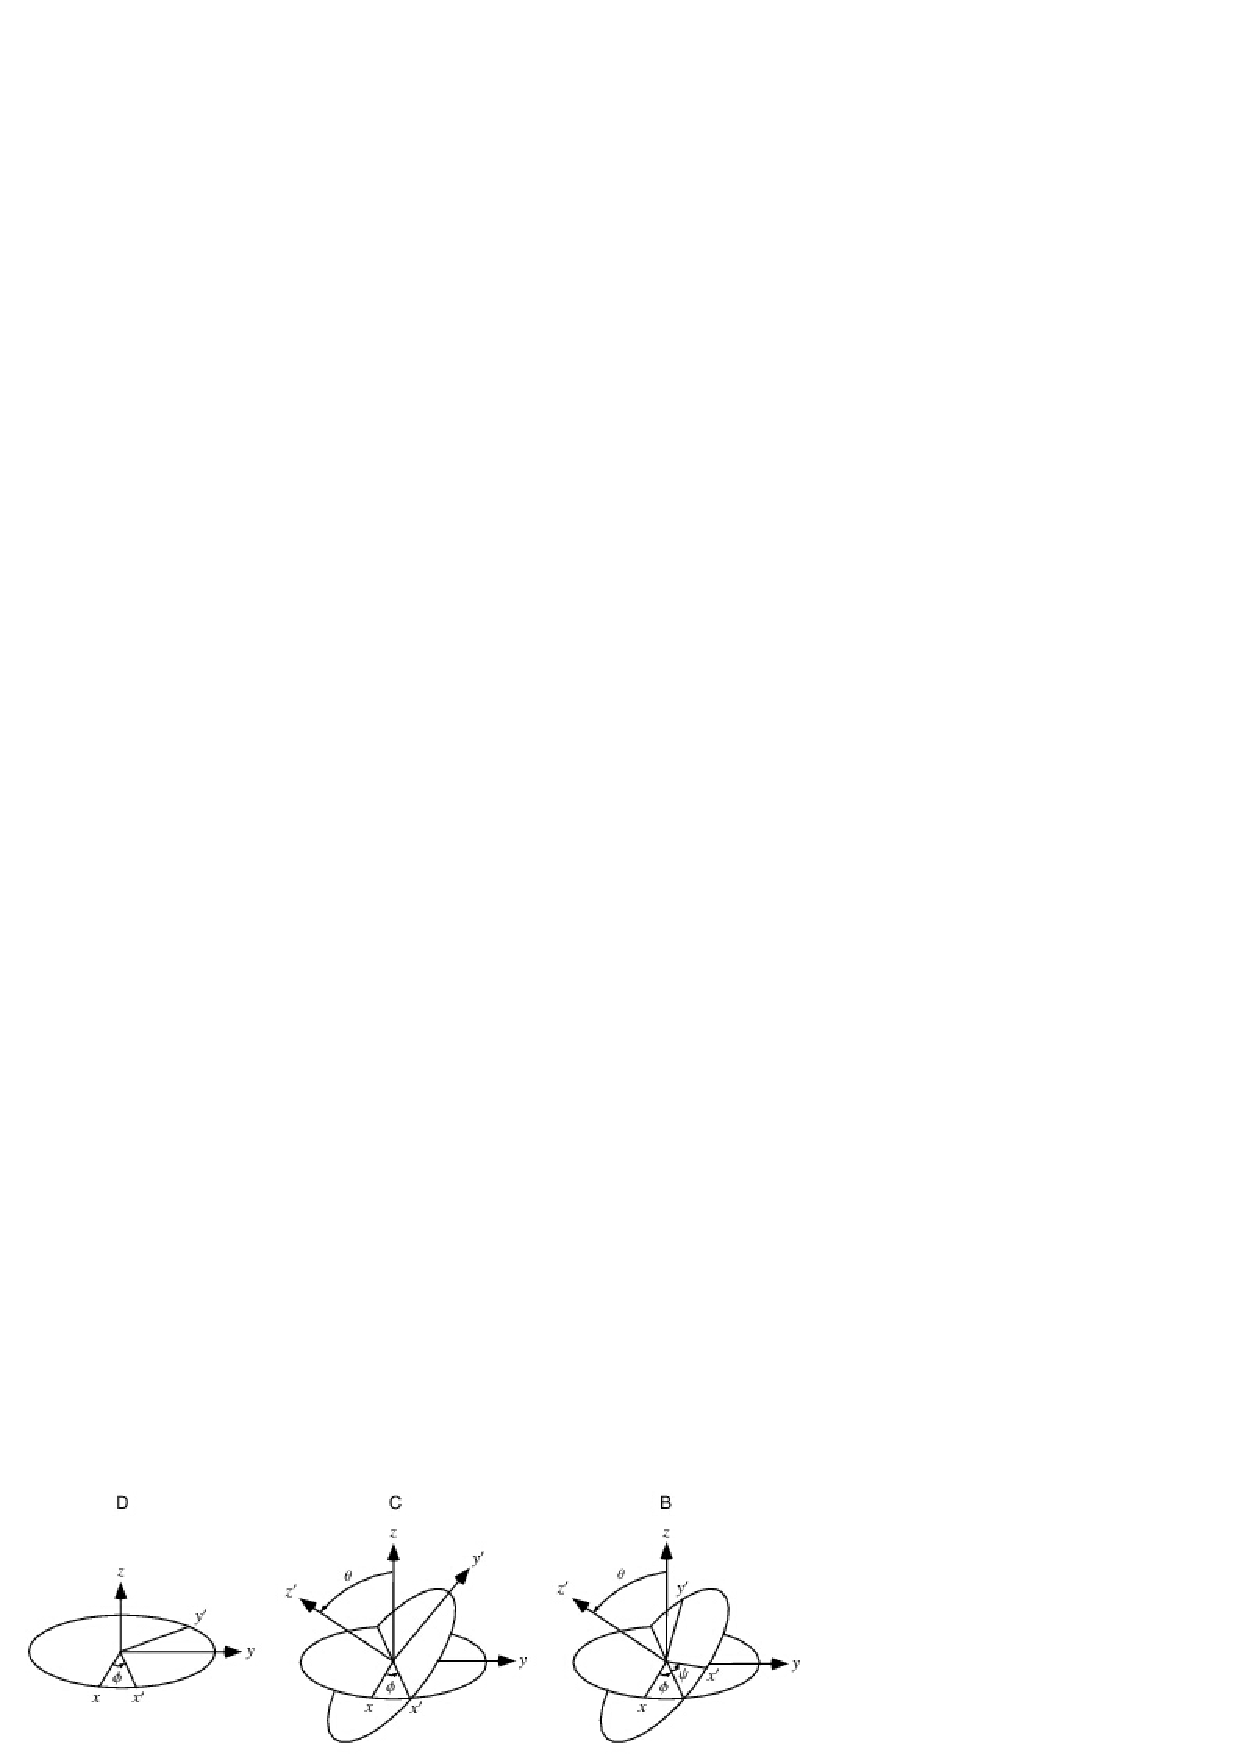
\includegraphics[width=0.96\columnwidth]{figures/euler_angles}
\caption{Demonstration of the Euler Angles. The first angle $\phi$ is with 
reapect to the $z$ axis; the second angle $\theta$ is with respect to the 
$x$ axis; the third angle $\psi$ is with repect to the $y$ axis.}
\label{fig:euler_angles}
\end{figure}

Each angle provides a rotation matrix.
\begin{equation}
D = \left(
    \begin{array}{ccc}
    \cos\phi & \sin\phi & 0 \\
    -\sin\phi & \cos\phi & 0 \\
    0 & 0 & 1 \\
    \end{array}
    \right),
C = \left(
    \begin{array}{ccc}
    1 & 0 & 0 \\
    0 & \cos\theta & \sin\theta \\
    0 & -\sin\theta & \cos\theta \\
    \end{array}
    \right),
B = \left(
    \begin{array}{ccc}
    \cos\psi & \sin\psi & 0 \\
    -\sin\psi & \cos\psi & 0 \\
    0 & 0 & 1 \\
    \end{array}
    \right)
\end{equation}
One thing that we need to keep in mind is that the order of the three 
rotations matters. Different order results in different final status. 
The composition of them $A=BCD$ is the rotation matrix
\begin{equation}
A = \left(
    \begin{array}{ccc}
    \cos\psi \cos\phi - \cos\theta \sin\phi \sin\psi & \cos\psi \sin\phi + \cos\theta \cos\phi \cos\psi & \sin\psi \sin \theta \\
    -\sin\psi \cos\phi - \cos\theta \sin\phi \cos\psi & -\sin \psi \sin\phi + \cos\theta \cos\phi \cos\psi & \cos\psi \sin\theta \\
    \sin\theta \sin\phi & -\sin\theta \cos\phi & \cos\theta \\
    \end{array}
    \right).
\label{eqn:rotation_matrix1}
\end{equation}
Angles are commonly defined according to the right hand rule. 
Namely, they have positive values when they represent a rotation that 
appears clockwise when looking in the positive direction of the axis, and 
negative values when the rotation appears counter-clockwise. 
About the ranges, $\phi$ and $\psi$ have a range of $2\pi$, and $\theta$ has 
a range of $\pi$. 



\section{Fluid Dynamics}
\label{Sec:FD}
Two most important set of governing equations that describe the motion 
of the fluid are Navier-Stokes equations and Euler equations. 
The basic method to derive both formulas is through principles of 
conservation of mass, momentum and energy
\cite{gonzalez2008continuum,lin1988mathapplied}.

\begin{itemize}
\item conservation of mass: 
\begin{equation}
\frac{\partial\rho}{\partial t}+\nabla\cdot\left(\rho\mathbf{u}\right)=0, 
\label{eqn:mass_con}
\end{equation}
where $\rho(\mathbf{x},t)$ is the spatial mass density field and 
$\mathbf{u}(\mathbf{x},t)$ is the associated spatial velocity field.
\item conservation of linear momentum:
\begin{equation}
\rho [\frac{\partial \mathbf{u}}{\partial t} + (\mathbf{u} \cdot \nabla) \mathbf{u}] = \nabla \cdot \mathbf{S} + \rho \mathbf{b}, 
\label{eqn:momentum_con}
\end{equation}
where $\mathbf{S}(\mathbf{x},t)$ is the Cauchy stress field and 
$\mathbf{b}(\mathbf{x},t)$ is the spatial body force per unit mass.
In addition, the conservation of angular momentum law leads to the 
symmetry constraint 
\begin{equation}
\mathbf{S}^{T}=\mathbf{S}.
\end{equation}
\item conservation of energy: 
\begin{equation}
\rho [\frac{\partial e}{\partial t} + (\mathbf{u} \cdot \nabla) e] = \nabla (\mathbf{S} \cdot \mathbf{u}) - \nabla \cdot \mathbf{q} + \rho r
\end{equation}
where $e(\mathbf{x},t)$ is the internal energy field per unit mass, 
$\mathbf{q}(\mathbf{x},t)$ is the Fourier-Stokes heat flux vector field, 
$r(\mathbf{x},t)$ is the heat supply field per unit mass.
\end{itemize}
Different choices of stress fields $\mathbf{S}(\mathbf{x},t)$ leads to 
equation for different type of fluid. 

\subsection*{Euler Equations}
In the world of ideal fluid which is inviscid, the Cauchy stress field is 
given as
\begin{equation}
\mathbf{S}(\mathbf{x},t) = -p(\mathbf{x},t)\mathbf{I}.
\end{equation}
Then, for the ideal fluid, in the case of absent extra body force, i.e. 
$\mathbf{b}(\mathbf{x},t) = 0$, Euler equation can be written as
\begin{eqnarray}
\left\{
\begin{aligned}
\frac{\partial \rho}{\partial t} + \nabla \cdot (\rho\mathbf{u}) &= 0 \\
\frac{\partial \mathbf{u}}{\partial t} + (\mathbf{u} \cdot \nabla) \mathbf{u} &= -\frac{1}{\rho} \nabla p \\
\frac{\partial E}{\partial t} + \nabla \cdot (\mathbf{u}(E + p)) &= 0, 
\end{aligned}
\right.
\label{eqn:Euler_eqns}
\end{eqnarray}
where $\rho$ is the fluid density, $\mathbf{u}$ is the velocity of
the fluid field, $p$ is the pressure, 
$E = \rho e + \frac{1}{2} \rho \mathbf{u}^{T} \mathbf{u}$
is the total energy density with $e$ being the specific internal
energy per unit mass. 

In order to make the system of equation closed, an equation of state is 
essential. 
Under classical ideal gas law, it can be expressed as 
\begin{equation}
p=\rho (\gamma -1) e, 
\label{eqn:equation_of_state}
\end{equation}
where $\gamma$ is the adiabatic index. 

With some algebric calculation, the momentum conservation can be 
rewritten in the conservative form 
\begin{equation}
\frac{\partial (\rho \mathbf{u})}{\partial t} + \nabla \cdot (\rho \mathbf{u} \mathbf{u}^{T} +  p\mathbf{I}) = 0,
\end{equation}
where $\mathbf{I}$ here is the $3\times3$ identity matrix.
Then, the Euler equations become a hyperbolic system when no external 
force is taken into account, 
\begin{equation}
\frac{\partial \mathbf{U}}{\partial t} + \frac{\partial \mathbf{F}(\mathbf{U})}{\partial x} + \frac{\partial \mathbf{G}(\mathbf{U})}{\partial y} + \frac{\partial \mathbf{H}(\mathbf{U})}{\partial z} = 0, 
\label{eqn:Euler_eqns_con}
\end{equation}
where 
\begin{equation}
\mathbf{U} = 
\left(
\begin{array}{c}
\rho \\ \rho u \\ \rho v \\ \rho w \\ E
\end{array}
\right),\ 
\mathbf{F} = 
\left(
\begin{array}{c}
\rho u \\ \rho u^2 + p \\ \rho u v \\ \rho u w \\ (E+p)u
\end{array}
\right),\ 
\mathbf{G} = 
\left(
\begin{array}{c}
\rho v \\ \rho u v \\ \rho v^2 + p \\ \rho v w \\ (E+p)v
\end{array}
\right),\ 
\mathbf{H} = 
\left(
\begin{array}{c}
\rho w \\ \rho u w \\ \rho v w \\ \rho w^2 + p \\ (E+p)w
\end{array}
\right)
\end{equation}

Due to the model assumption, Euler equation is most appropriate for 
simulating compressible inviscid fluid which has large Reynolds number, 
such as bullet ejection, spacecraft entrance and so on.

\subsection*{Navier-Stokes Equations}
In the incompressible Newtonian fluid case, mass density field
is uniform which means it is constant $\rho$ in the field. Thus,
\Eqn{mass_con} implies the so-called divergence-free condition 
\begin{equation}
\nabla \cdot \mathbf{u}=0.
\end{equation}
The Newtonian Cauchy stress field is given as
\begin{equation}
\mathbf{S}(\mathbf{x},t) = -p(\mathbf{x},t) \mathbf{I} + \mu (\nabla \mathbf{u}(\mathbf{x},t) + \nabla \mathbf{u} (\mathbf{x},t)^{T}), 
\end{equation}
where $\mu$ is dynamic viscosity. 

Considering only the gravitational force, i.e. 
$\mathbf{b}(\mathbf{x},t) = \mathbf{g}$, Navier-Stokes equations for 
incompressible Newtonian fluid can be rewritten as 
\begin{eqnarray}
\left\{
\begin{aligned}
\nabla \cdot \mathbf{u} &= 0 \\
\frac{\partial \mathbf{u}}{\partial t} + (\mathbf{u} \cdot \nabla) \mathbf{u} &= -\frac{1}{\rho} \nabla p + \nu \nabla^{2} \mathbf{u} + \mathbf{g}
\end{aligned}
\right.
\label{eqn:navierstoke_eqns}
\end{eqnarray}
where $\nu = \mu / \rho$ is the kinematic viscosity and $\rho_{0}$ is the 
fluid density, $\mathbf{u}$ is the velocity of the fluid field, $p$ is the
pressure. 

Due to the incompressible and viscous assumption, Navier-Stokes
equations have wide applications in physics, geoscience, aerospace and
even medical simulation when coupled with certain boundary conditions
and other appropriate constraints.



\section{Spring-Mass Model}
\label{Section:SMM}
Using spring system to model the dynamic motion of fabric surface has been
studied by computer scientists and applied mathematicians in the past several
decades, such as \cite{Choi02,Hsiao06,Ji06,Aileni10}.
Its main advantage is its simplicity and easy implementation.
We built our spring-mass model with similar idea to \cite{Choi02} and improved
it with Delingette's modification \cite{TriangularSM} to simulate the parachute
canopy.

Triangulized mesh is adopted to represent the surface where the edges of
those triangles are springs and the vertices are mass points, as shown in 
\Fig{tri_mesh}.
\begin{figure}[!ht]
    \centering
    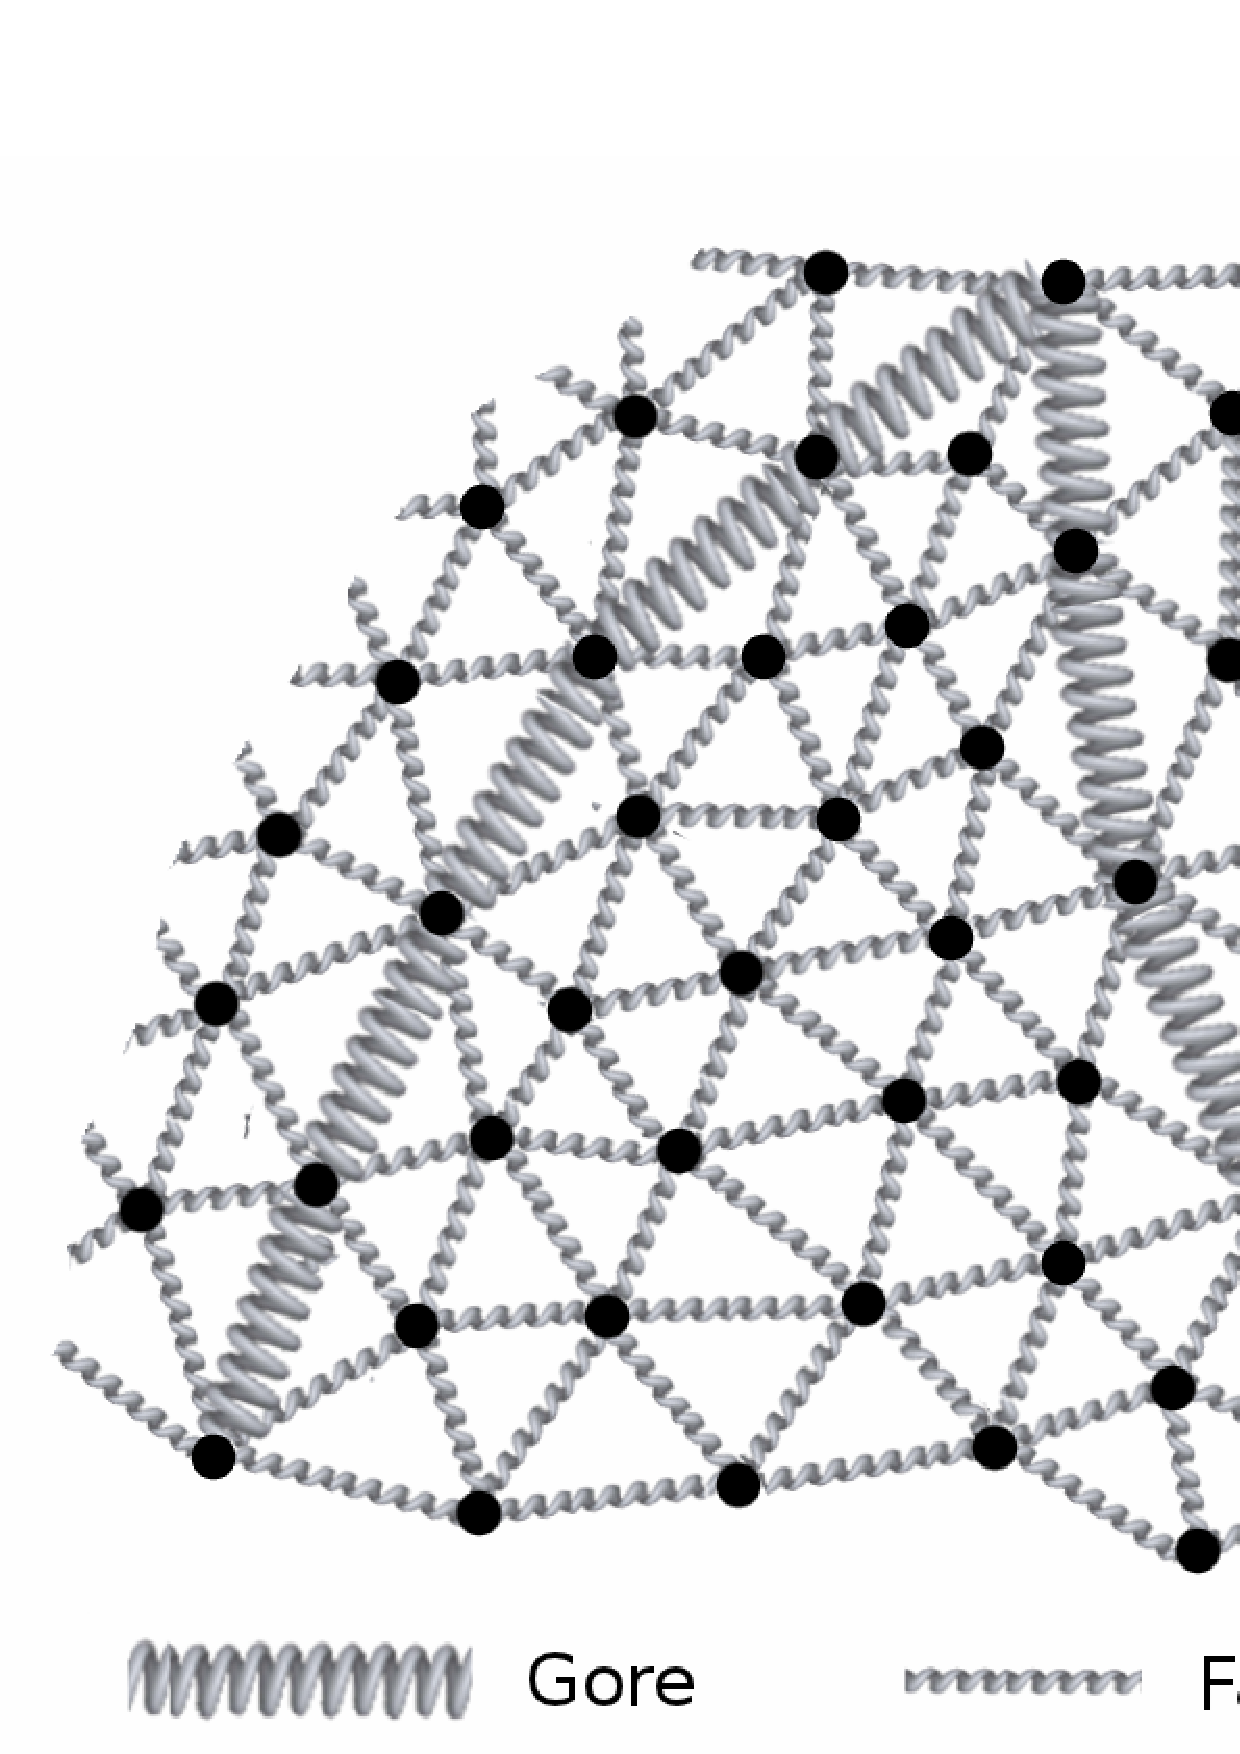
\includegraphics[width=0.6\columnwidth]{figures/goremesh}
    \caption{The spring model on a triangulated mesh. Each vertex point in
    the mesh represents a mass point with point mass $m$. Each edge of a
    triangle has a tensile stiffness. With the equilibrium lengths set during
    the initialization, the changing length of each side exerts a tensile
    spring force on the two neighboring vertex in opposite directions. Gore
    boundaries used in the parachute system can be added and modeled by curves
    with a different tensile stiffness.}
    \label{fig:tri_mesh}
\end{figure}
For each spring vertex in the spring-mass model, its motion is governed by
Newton's second law
\begin{equation}
m_{i} \frac{d\dot{\mathbf{X}}_{i}}{dt} = \mathbf{F}_i,\ i = 1,2,\cdots,N, 
\label{eqn:sm_motion}
\end{equation}
where $m_{i}$ is the mass, $\mathbf{X}_{i}$ is the position,  and
$\mathbf{F}_i$ is the total force inserted on the spring vertex.

In a elastic structure dynamics simulation, $\mathbf{F}_i$ consists of a
force $\mathbf{F}_{i}^{s}$ due to the deformation of triangles and a damping
force which slows the motion of the spring system due to friction
$\mathbf{F}_{i}^{d}$.
The external force $\mathbf{F}_{i}^{e}$, representing the effects of air drag
and gravity is considered by adding an additional term on the right-hand side.

Our spring-mass model \cite{LiChernKimLi12,shi2015verification} assumes the
force to stretch the spring is proportional to its displacement from the
equiblibrium distance between the two adjacent spring vertices.
In addition, the force that prevents the change of angles is described by the
angular stiffness in Delingette's modification \cite{TriangularSM} which is
favored by its relation to the elastic spring model in continuum mechanics.
\begin{figure}
\centering
\begin{subfigure}{0.48\columnwidth}
    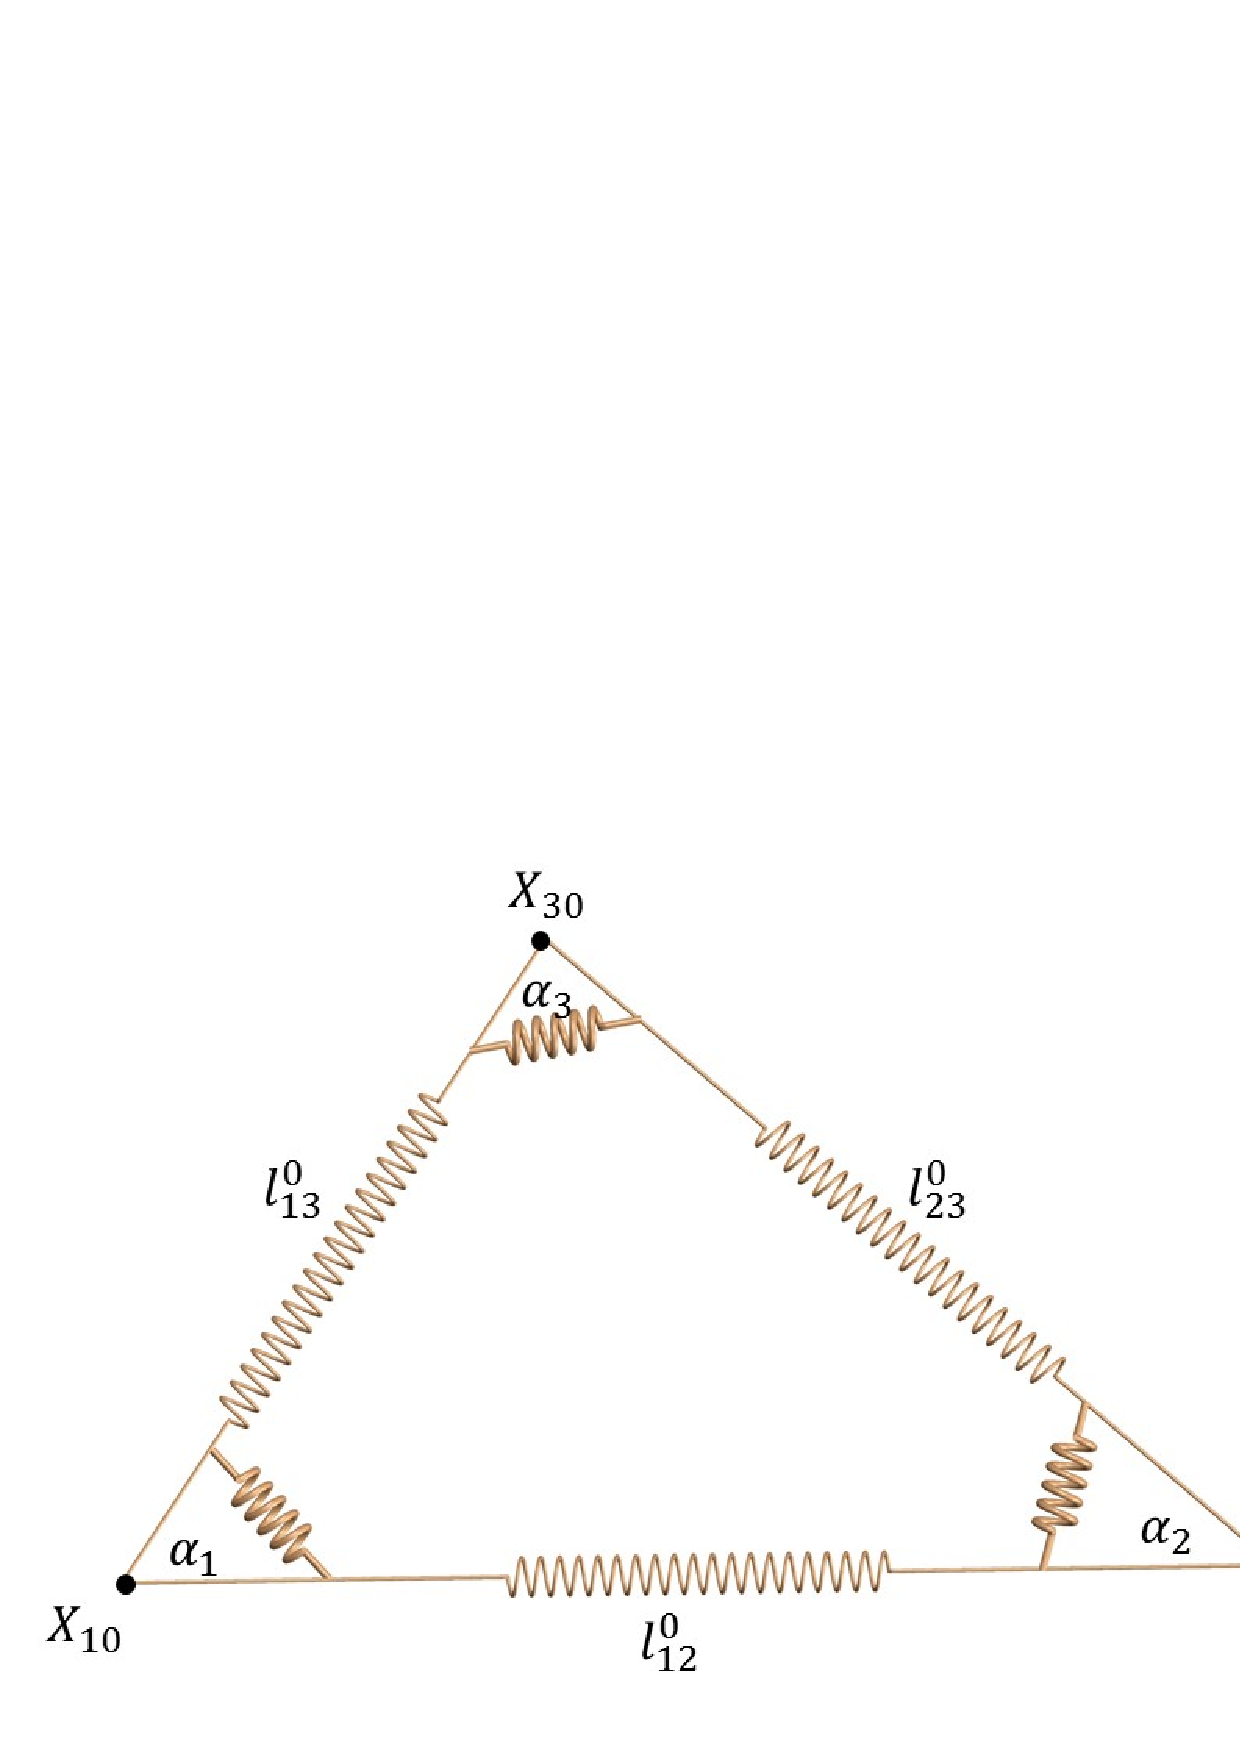
\includegraphics[width=1.0\textwidth]{figures/rest}
    \caption{Triangle in the rest status}
\end{subfigure}
\begin{subfigure}{0.48\columnwidth}
    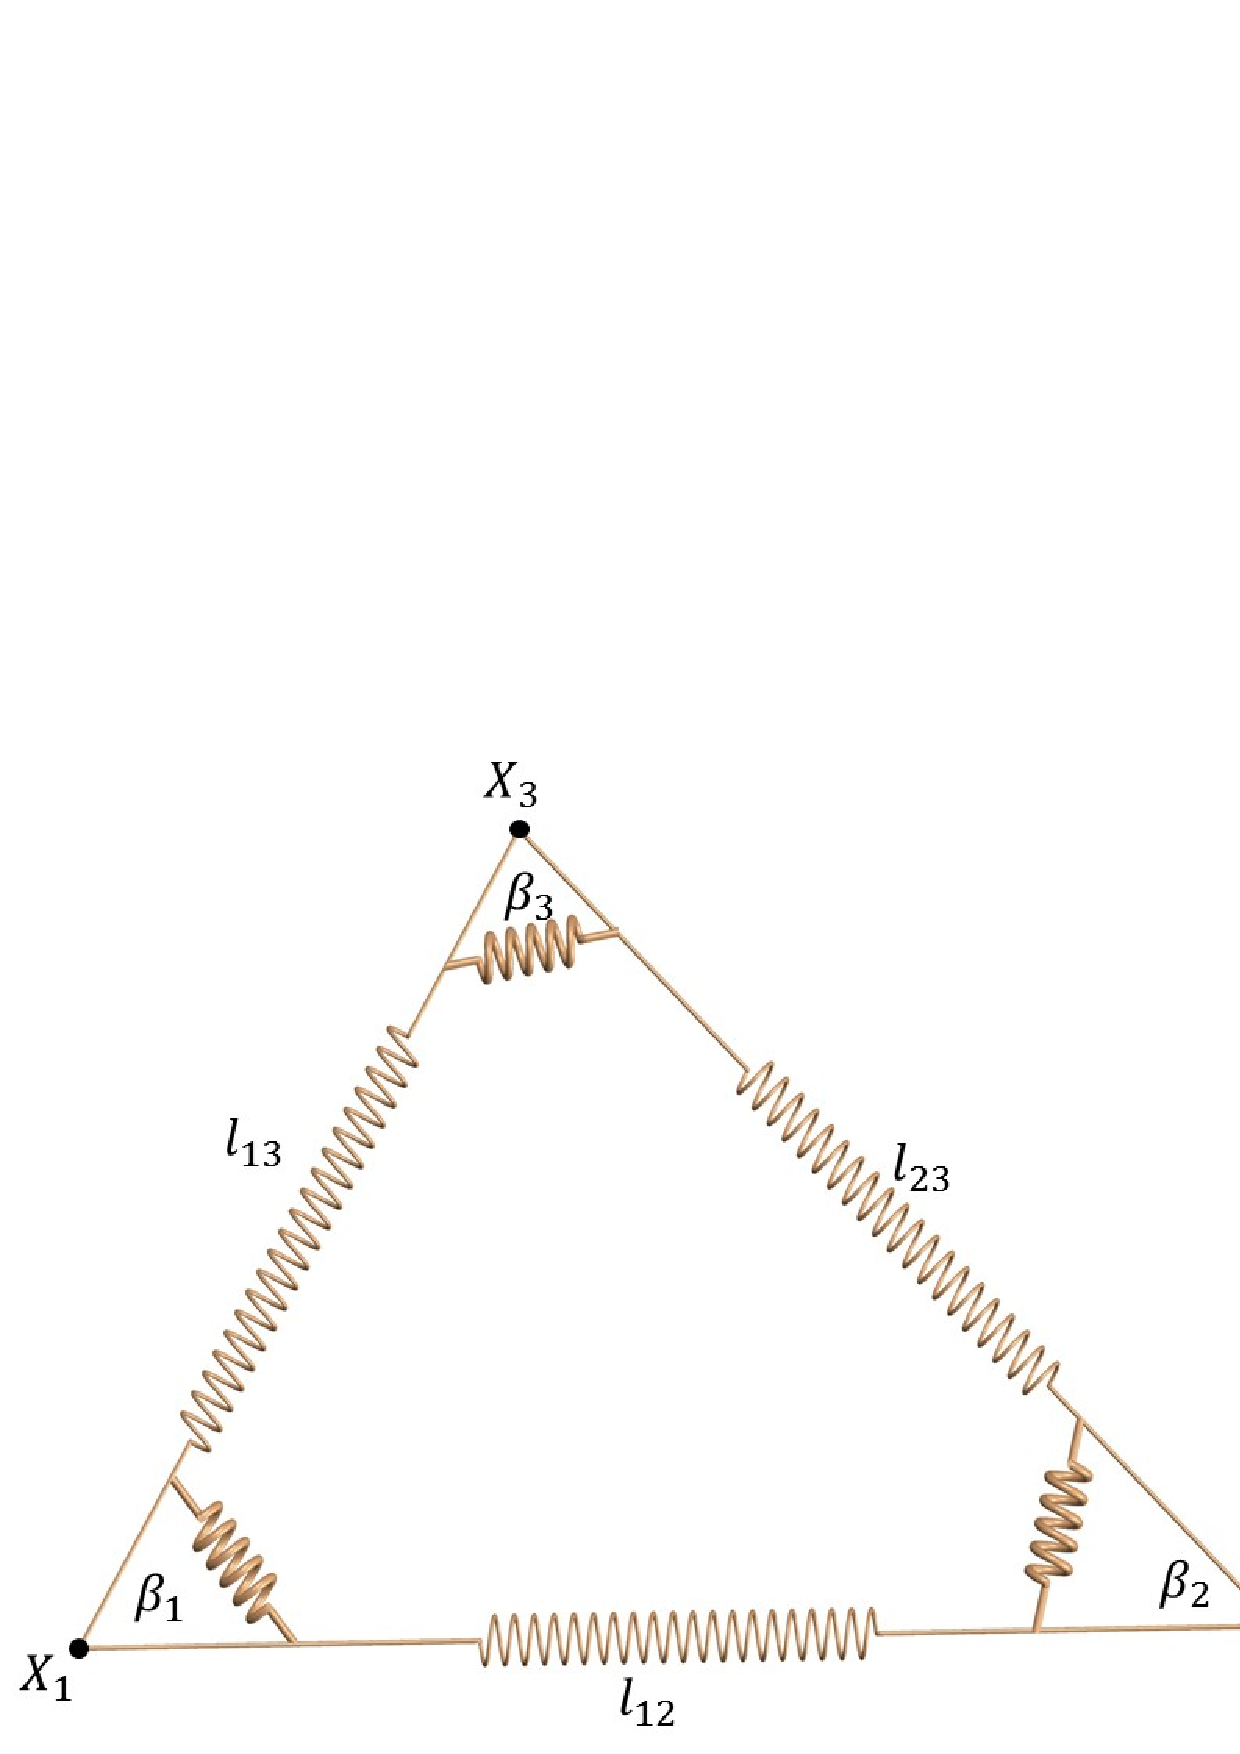
\includegraphics[width=1.0\textwidth]{figures/deformed}
    \caption{Triangle in the deformed status}
\end{subfigure}
\caption{Left: rest triangle $T_{X_0}$ with vertex $X_{i0}$. Right:
deformed triangle $T_{X}$ with vertex $X_{i}$. Each edge is represented as
a spring and the tensile stiffness prevents the deformation of the edge.
At each corner, an artifical spring prevents the change of angles.}
\label{fig:rest_deformed_tri}
\end{figure}

With $dl_{ij} = l_{ij} - l_{ij}^0$ representing the length change of the
spring between $\mathbf{X}_{i}$ and $\mathbf{X}_{j}$, the potential energy
is given in \cite{TriangularSM} as
\begin{equation}
W(T) = \sum_{\substack{i=1\\j=(i+1) \mod 3}}^{3}\frac{1}{2}k_{ij}^{T}(dl_{ij})^{2} + \sum_{\substack{i=1\\j=(i+1) \mod 3\\k=(i+2) \mod 3}}^{3}\gamma_{i}^{T}dl_{ij}dl_{ik}, 
\label{eqn:sm_energy}
\end{equation}
where the first term is the stretching energy, and the second term is the
angular energy from Delingette's modification.

In \Eqn{sm_energy}, the tensile stiffness and the angular stiffness are
calculated as
\begin{equation}
k_{ij}^{T} = \frac{(l_{ij}^0)^2 (2\cot^2\alpha_k(\lambda+\mu)+\mu)}{8A}, 
\label{eqn:t_stiffness}
\end{equation}
\begin{equation}
\gamma_{i}^{T} = \frac{l_{ik}^0 l_{ij}^0 (2 \cot\alpha_j \cot\alpha_k (\lambda+\mu) - \mu)}{8A},
\label{eqn:a_stiffness}
\end{equation}
where $A$ denotes the area of the triangle in equilibrium, $i = 1,2,3$,
$j = (i+1)\ \mod\ 3$, and $k = (i+2)\ \mod\ 3$.
$\lambda$ and $\mu$ are the Lam\'{e} coefficients of the material, and they
are related to Young's modulus $E$ and the Poisson ratio $\nu$ \cite{Gere2004}
\begin{equation}
\lambda=\frac{E\nu}{1-\nu^2},\ \mu=\frac{E(1-\nu)}{1-\nu^2}.
\label{eqn:Lame_coeff}
\end{equation}

Apply Rayleigh-Ritz analysis and it tells that the fabric surface, represented
by the triangular mesh, should evolve by minimizing its membrane energy.
Therefore, along the opposite derivative of that energy with respect to the
nodes of the system, that is, the deformed positions $X_i$:
\begin{align}
\mathbf{F}_{i}^{s}(T_{\mathbf{X}_{0}}) &=  -\frac{\partial W(T_{\mathbf{X}_{0}})}{\partial \mathbf{X}_{i}} \notag \\
&= \sum_{\substack{j=1\\j\neq i}}^{3} k_{ij}^{T_{\mathbf{X}_{0}}} dl_{ij} \frac{\mathbf{X}_{j}-\mathbf{X}_{i}}{l_{ij}} + 
\sum_{\substack{j=1,j\neq i\\k\neq i,k\neq j}}^{3} (\gamma_{k}^{T_{\mathbf{X}_{0}}} dl_{kj} + \gamma_{i}^{T_{\mathbf{X}_{0}}}dl_{ij}) \frac{\mathbf{X}_{k}-\mathbf{X}_{i}}{l_{ik}}
\label{eqn:tri_sm_force}
\end{align}
This is the force on vertex $\mathbf{X}_{i}$ due to the deformation of the
triangular $T_{\mathbf{X}_{0}}$ and it can be split into two components
\begin{equation}
\mathbf{F}_{i}^{s}(T_{\mathbf{X}_{0}}) = \mathbf{F}_{ij}^{s}(T_{\mathbf{X}_{0}}) + \mathbf{F}_{ik}^{s}(T_{\mathbf{X}_{0}}),
\end{equation}
where $j=(i+1)\ mod\ 3$ and $k=(i+2)\ mod\ 3$, and
\begin{align}
\mathbf{F}_{ij}^{s}(T_{\mathbf{X}_{0}}) &= k_{ij}^{T_{\mathbf{X}_{0}}} dl_{ij} \mathbf{e}_{ij} + (\gamma_i^{T_{\mathbf{X}_{0}}} dl_{ik} + \gamma_{j}^{T_{\mathbf{X}_{0}}} dl_{jk}) \mathbf{e}_{ij}, \\
\mathbf{F}_{ik}^{s}(T_{\mathbf{X}_{0}}) &= k_{ik}^{T_{\mathbf{X}_{0}}} dl_{ik} \mathbf{e}_{ik} + (\gamma_i^{T_{\mathbf{X}_{0}}} dl_{ij} + \gamma_{k}^{T_{\mathbf{X}_{0}}} dl_{kj}) \mathbf{e}_{ik}.
\end{align}
\begin{figure}[!ht]
    \centering
    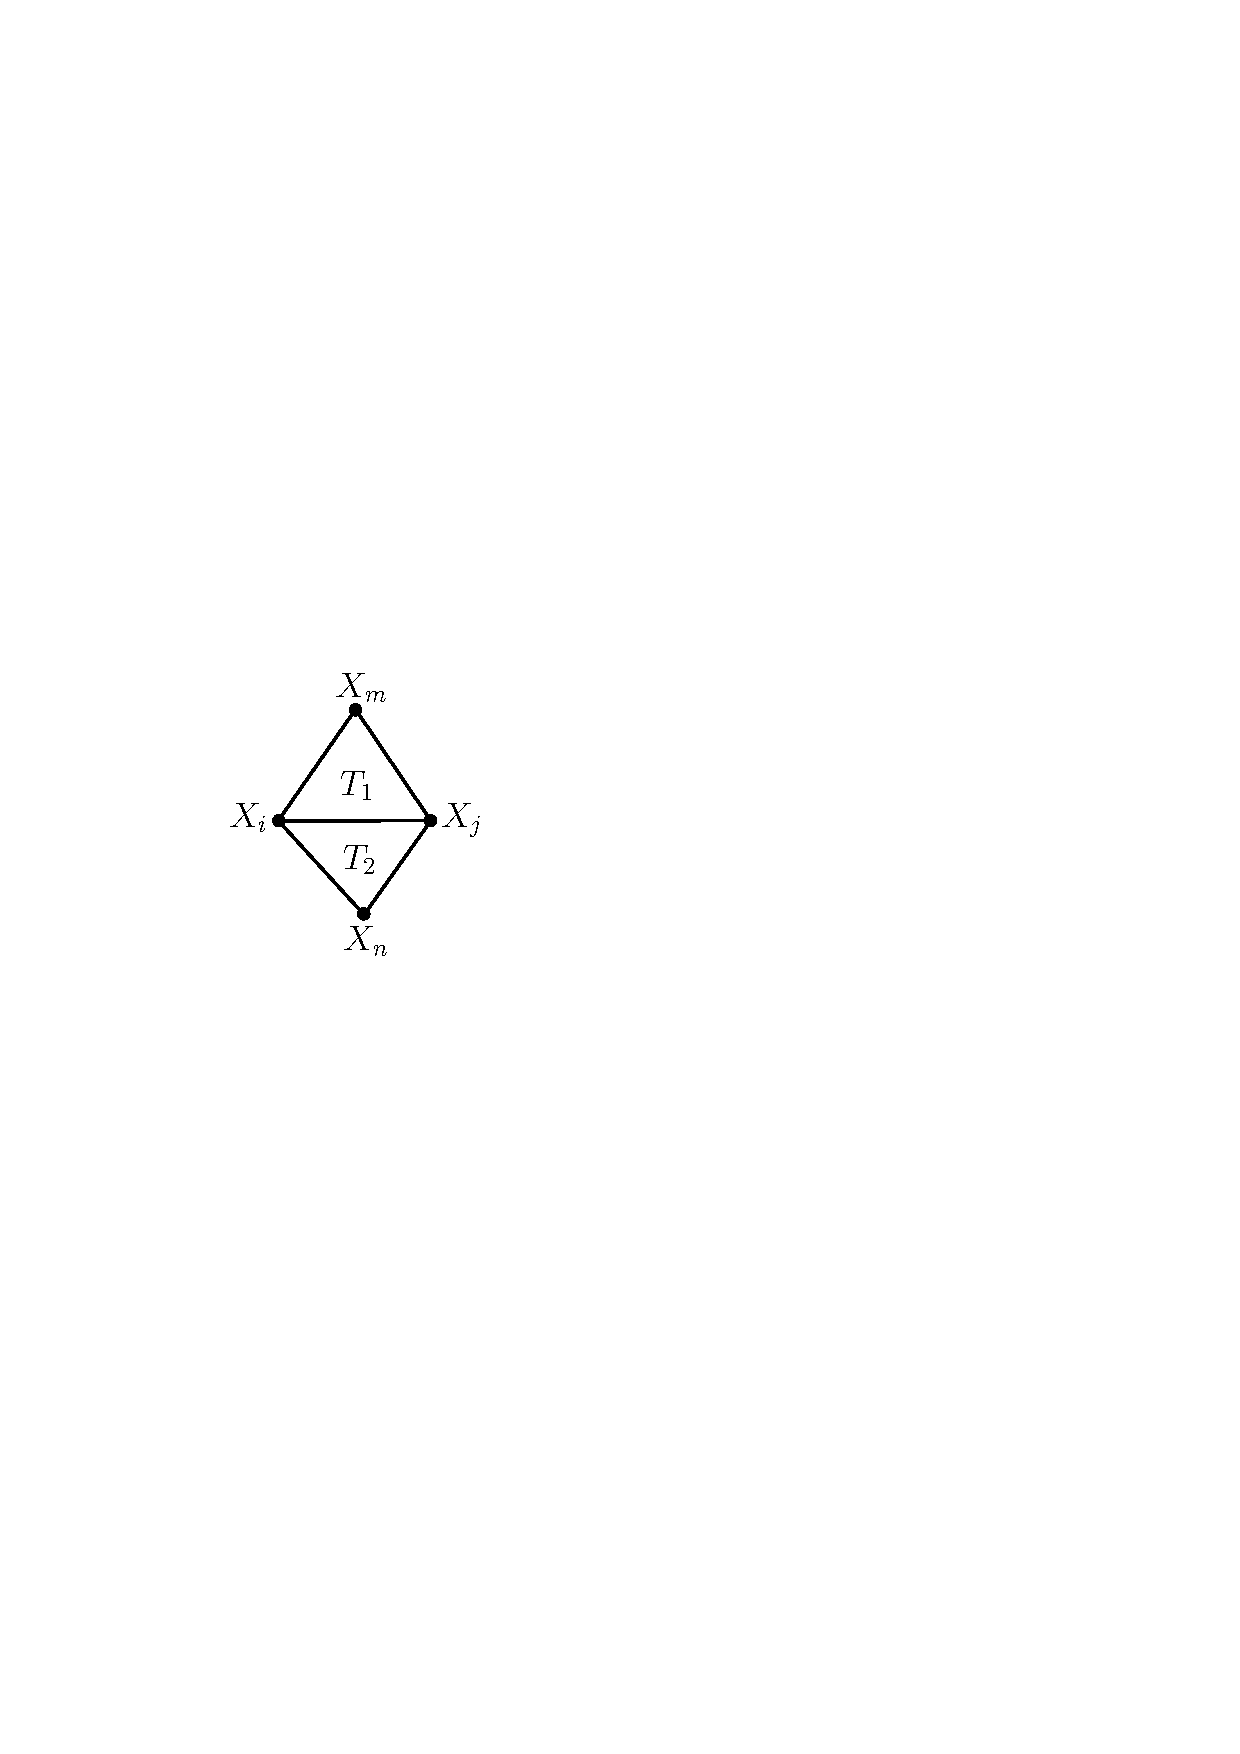
\includegraphics[width=0.4\columnwidth]{figures/force_ij}
    \caption{Two triangles $T_1$ and $T_2$ share $\mathbf{X}_i$ and
    $\mathbf{X}_j$; the other vertex of triangles $T_1$ and $T_2$ are
    $\mathbf{X}_m$ and $\mathbf{X}_n$ respectively.}
    \label{fig:force_ij}
\end{figure}

Since each edge is shared by two triangles, the spring force between two vertex
$\mathbf{X}_i$ and $\mathbf{X}_j$, as shown in \Fig{force_ij}, is the
summation of the effects from both triangles and has
the following formula:
\begin{align}
\mathbf{F}_{ij}^{s} &= \mathbf{F}_{ij}^{s}(T_1) + \mathbf{F}_{ij}^{s}(T_2) \notag \\
&= [(k_{ij}^{T_1} + k_{ij}^{T_2})dl_{ij} + (\gamma_{i}^{T_1}dl_{im} + \gamma_{j}^{T_1}dl_{jm} + \gamma_{i}^{T_2}dl_{in} + \gamma_{j}^{T_2}dl_{jn})]\mathbf{e}_{ij} \notag \\ 
&= \tilde{k}_{ij}dl_{ij}\mathbf{e}_{ij} + \tilde{\gamma}_{ij}dl_{ij}\mathbf{e}_{ij},
\label{eqn:sm_force_new}
\end{align}
where $\tilde{k}_{ij} = k_{ij}^{T_1}+k_{ij}^{T_2}$, $\tilde{\gamma}_{ij} = 
(\gamma_{i}^{T_1}dl_{im} + \gamma_{j}^{T_1}dl_{jm} + \gamma_{i}^{T_2}dl_{in} + 
\gamma_{j}^{T_2}dl_{jn})/dl_{ij}$.

As mentioned earlier, a damping force slows the spring system and we take it
into account with the formula
\begin{equation}
\mathbf{F}_{i}^{d} = c \mathbf{V}_{i}^{(int)},
\label{eqn:damp_force}
\end{equation}
where $c$ is the viscous damping coefficient and $\mathbf{V}_{i}^{(int)}$ is
the internal component of the vertex velocity that is due to the spring force
only.
On the other hand, the external component $\mathbf{V}_{i}^{(ext)}$ involves
effects from gravity, fluid, and so on.
With all forces considered, the equation of motion (\ref{eqn:sm_motion}) can
be re-written as an ODE system
\begin{equation}
\left\{
\begin{aligned}
\dot{\mathbf{X}}_{i} &= \mathbf{V}_{i} \\
m_{i} \dot{\mathbf{V}}_{i} &= \mathbf{F}_{i}^{s} + \mathbf{F}_{i}^{d} + \mathbf{F}_{i}^{e}
\end{aligned}
\right.
\label{eqn:sm_ODEs}
\end{equation}
where $\mathbf{V}_{i}$ is the total velocity, i.e. the summation of
$\mathbf{V}_{i}^{(int)}$ and $\mathbf{V}_{i}^{(ext)}$.

One thing that we need to keep in mind is that the canopy-like structures
are lack of bending stiffness, therefore, the bending force can be negligible
in the simulation of the parachute system.
However, for simulations of other kind of fabric structures, bending force
can be taken into account by adding an artificial spring between the two
vertex, $\mathbf{X}_{m}$ and $\mathbf{X}_{n}$, that are not shared by two 
adjacent triangles.
This additional resistance prevents local clustering of triangle meshes.



\section{Parachutist/Cargo Inclusion}
\label{PCI}
The dimensions of parachutist or cargo are usually smaller than the parachute
canopy surface.
However, when the fluid flow across the parachutist or cargo, the dynamical
behavior of the flow will have different patterns based on different Reynolds
numbers.
These turbulent flow will reach the parachute canopy surface later and
contribute to the motion of the canopy surface.
Therefore the inclusion of parachutists will make numerical simulation of
parachute systems much closer to reality.
\Fig{cargo_amplification} show three examples of connecting the suspension 
lines to the parachutist.
\begin{figure}
\centering
\begin{subfigure}{0.32\columnwidth}
    \includegraphics[width=1.0\textwidth]{figures/box}
    \caption{A cuboid cargo}
\end{subfigure}
\begin{subfigure}{0.32\columnwidth}
    \includegraphics[width=1.0\textwidth]{figures/ball}
    \caption{A spherical cargo}
\end{subfigure}
\begin{subfigure}{0.32\columnwidth}
    \includegraphics[width=1.0\textwidth]{figures/human}
    \caption{Human parachutist}
\end{subfigure}
\caption{Three examples of the connection amplification between the 
suspension lines and different types of cargos. Besides these three, 
\FronTierp is capable of generating different kinds of rigid bodies.}
\label{fig:cargo_amplification}
\end{figure}

In our model, the parachutist can be either a mass point with no instance or
a rigid body with finite volume.
In the former case, no interaction between the parachutist and the fluid is
considered.
Therefore, no turbulent flow is observed between the space of the canopy
surface and the parachutist.
However, in the latter case, the fluid-structure interaction is non-negligible,
and there are two important aspects need to be taken into account carefully.
\begin{itemize}
\item Calculation of force and torque on the cargo. \\
    The force consists of three parts: force of gravity, force exerted by the
    fluid flow and force from the suspension lines.
    The force and corresponding torque are then applied to the parachutist for
    translation and rotation.
    \begin{itemize}
    \item The force exerted by the fluid flow can be broken into two parts:
    force due to pressure difference and force due to friction (viscosity).
    In the parachute simulation, we consider the first part as the dominant
    component.
    \begin{eqnarray}
    \begin{aligned}
    F_p &= \int_{s} (p - p_0)\hat{n} dA, \\
    \end{aligned}
    \end{eqnarray}
    where $\hat{n}$ is the normal direction to the surface with area $dA$,
    $p_0$ is the pressure far away from the surface $dA$
    and $p$ is the pressure at surface $dA$.
    \end{itemize}
\item Propagation of the rigid body. \\
    The propagation must maintain the geometric shape of the parachutist.
    This has perfect match with the Lagrangian propagation of the front
    tracking method in \FronTierp \cite{GliGroLi99a,DuFixGli05}.
    \begin{itemize}
    \item The translational motion is trivial.
    Simply apply the acceleration caused by the total force to the center of
    mass, and correspondingly propagate each point of the parachutist.
    \item The rotational motion with respect to the center of mass is governed
    by Euler's equations \Eqn{eulers_equation2} of rigid body dynamics
    \cite{goldstein2001}.
    \end{itemize}
\end{itemize}



\section{Collision Handling}
\label{Sec:CH}
In cloth simulations, it is almost impossible to totally avoid collision. 
Thus, robust collision detection and handling is very important to make the 
numerical simulation visually realistic. 
The collision detection and handling problem has attracted scientists in 
many fields. 
Early work by Terzopoulosi \emph{et al.}, \cite{terzopoulos1987elastically, 
terzopoulos1988modeling, terzopoulos1991deformable}, is governed 
by the mechanical laws of continuous bodies. 
Since then, many well-performed and well-known techniques are proposed by 
different groups, like Carignan \emph{et al.} \cite{carignan1992dressing}, 
Volino \emph{et al.} \cite{volino1995collision, volino1995versatile, 	volino1996evolving}, Baraff \emph{et al.} \cite{baraff1998large, 
baraff2003untangling}, Bridson \emph{et al.} \cite{Bridson2002collsn} and 
so on.  
Our collision algorithm is mainly based on the idea of combining a fail-safe 
geometric collision method and the repulsion force method that is presented 
in \cite{Bridson2002collsn}. 
In addition, we extended this algorithm to make it work for not only cloth, 
but also strings and rigid bodies.

In \Fig{collsn_demo}, the process of the collision algorithm is 
demonstrated for collision between fabric structure and a static object. 
As for self-collision of the fabric structure and collision between fabric 
structure and a movable object, the handling is similar. 
The only difference lies in how they move back to the time right before 
collision and how the impulse is applied.
\begin{figure}[!ht]
    \centering
    \begin{subfigure}{0.48\columnwidth}
	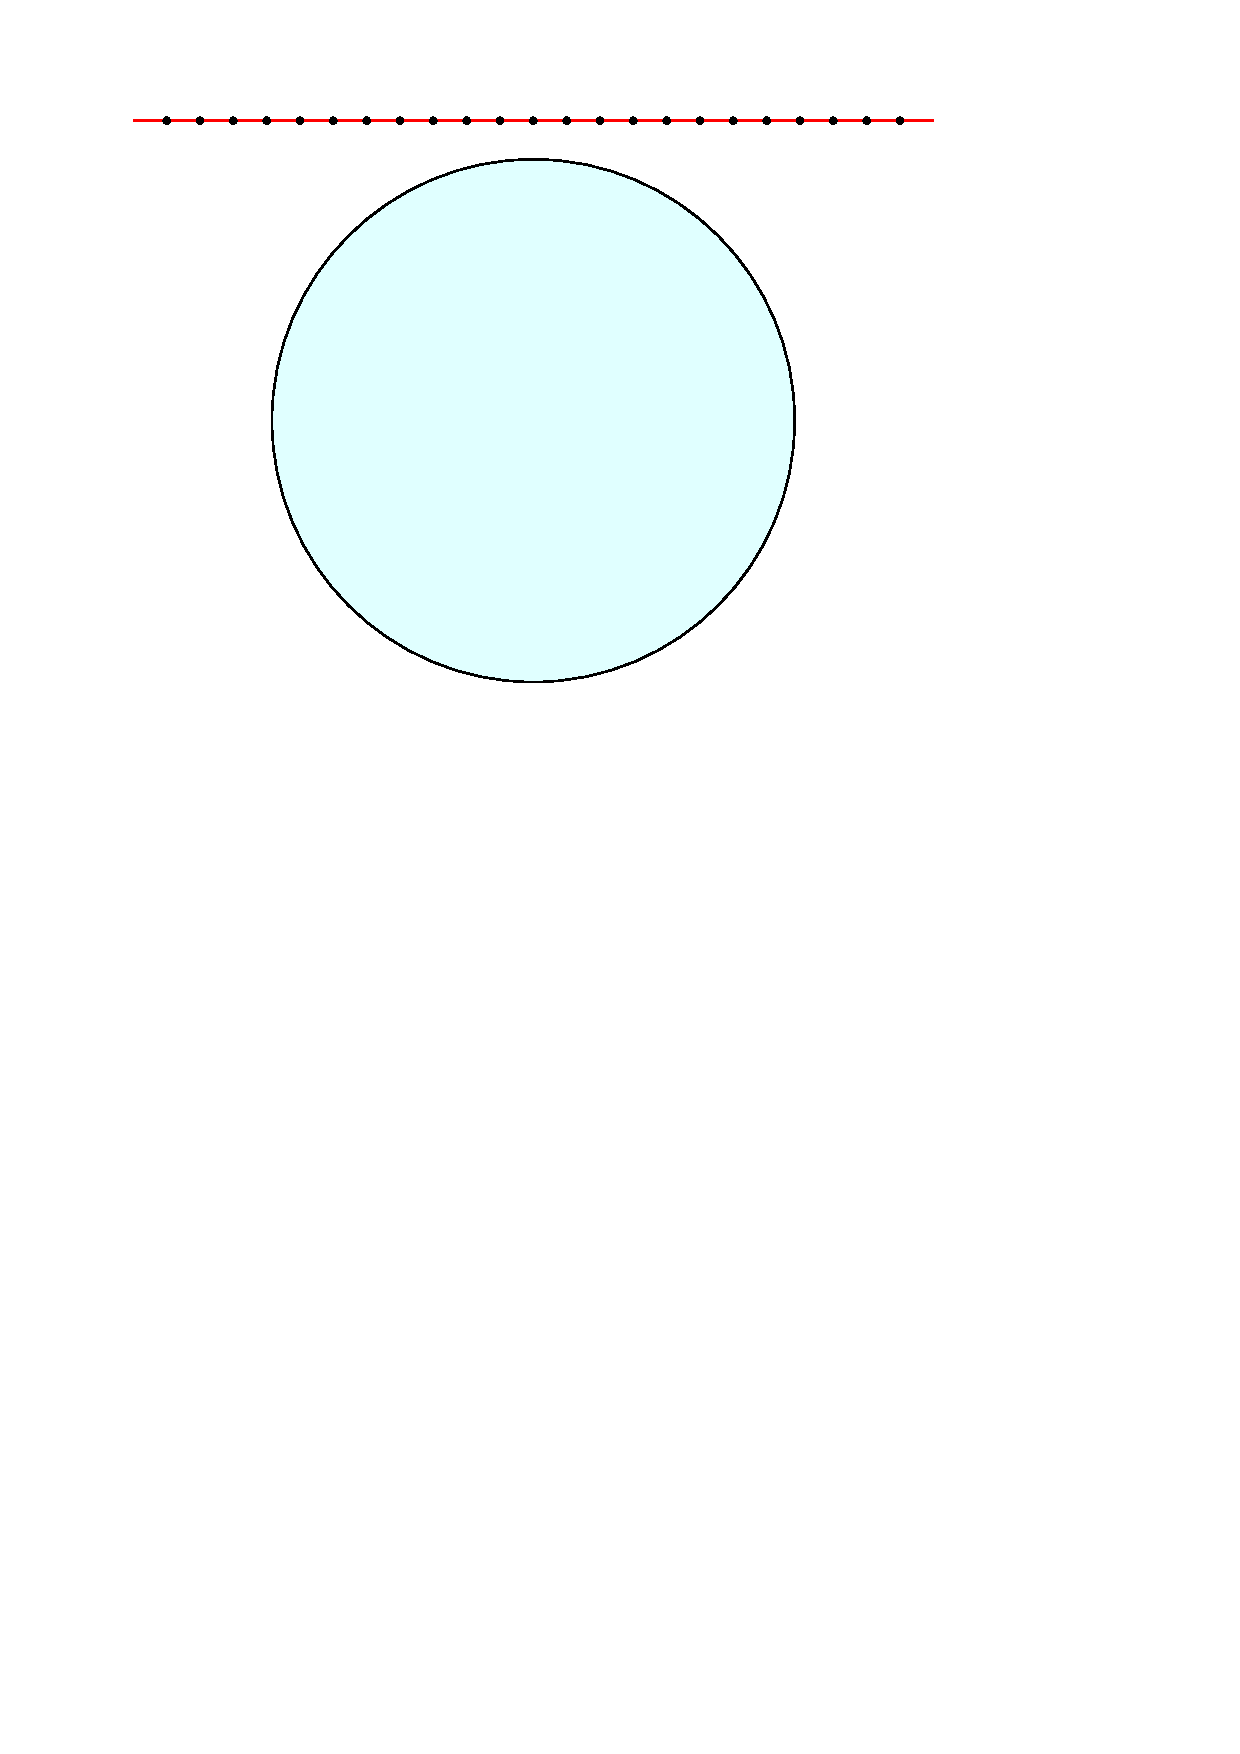
\includegraphics[width=\textwidth]{figures/collsn_demo_0}
	\caption{before collision}
    \end{subfigure}
    \begin{subfigure}{0.48\columnwidth}
	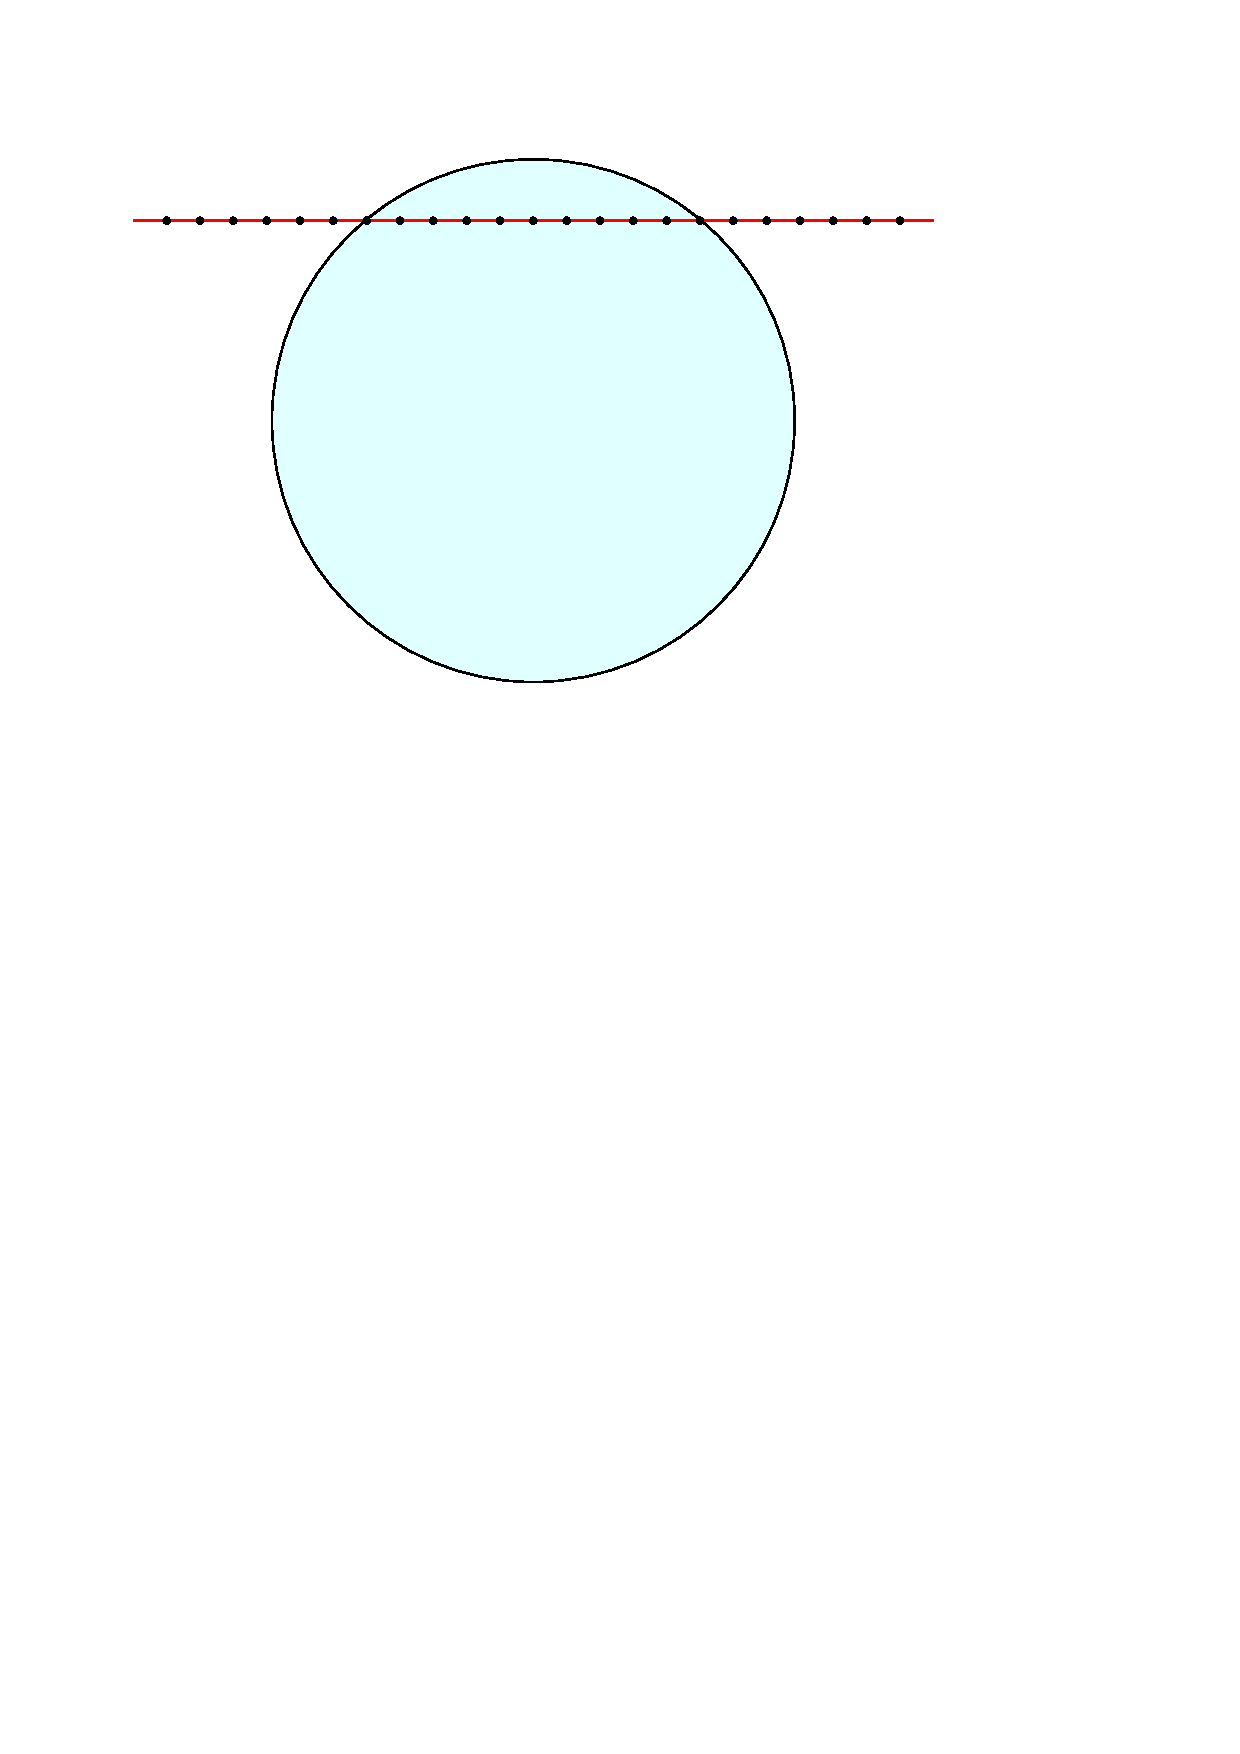
\includegraphics[width=\textwidth]{figures/collsn_demo_1}
	\caption{collision occurs}
    \end{subfigure} \\
    \begin{subfigure}{0.48\columnwidth}
	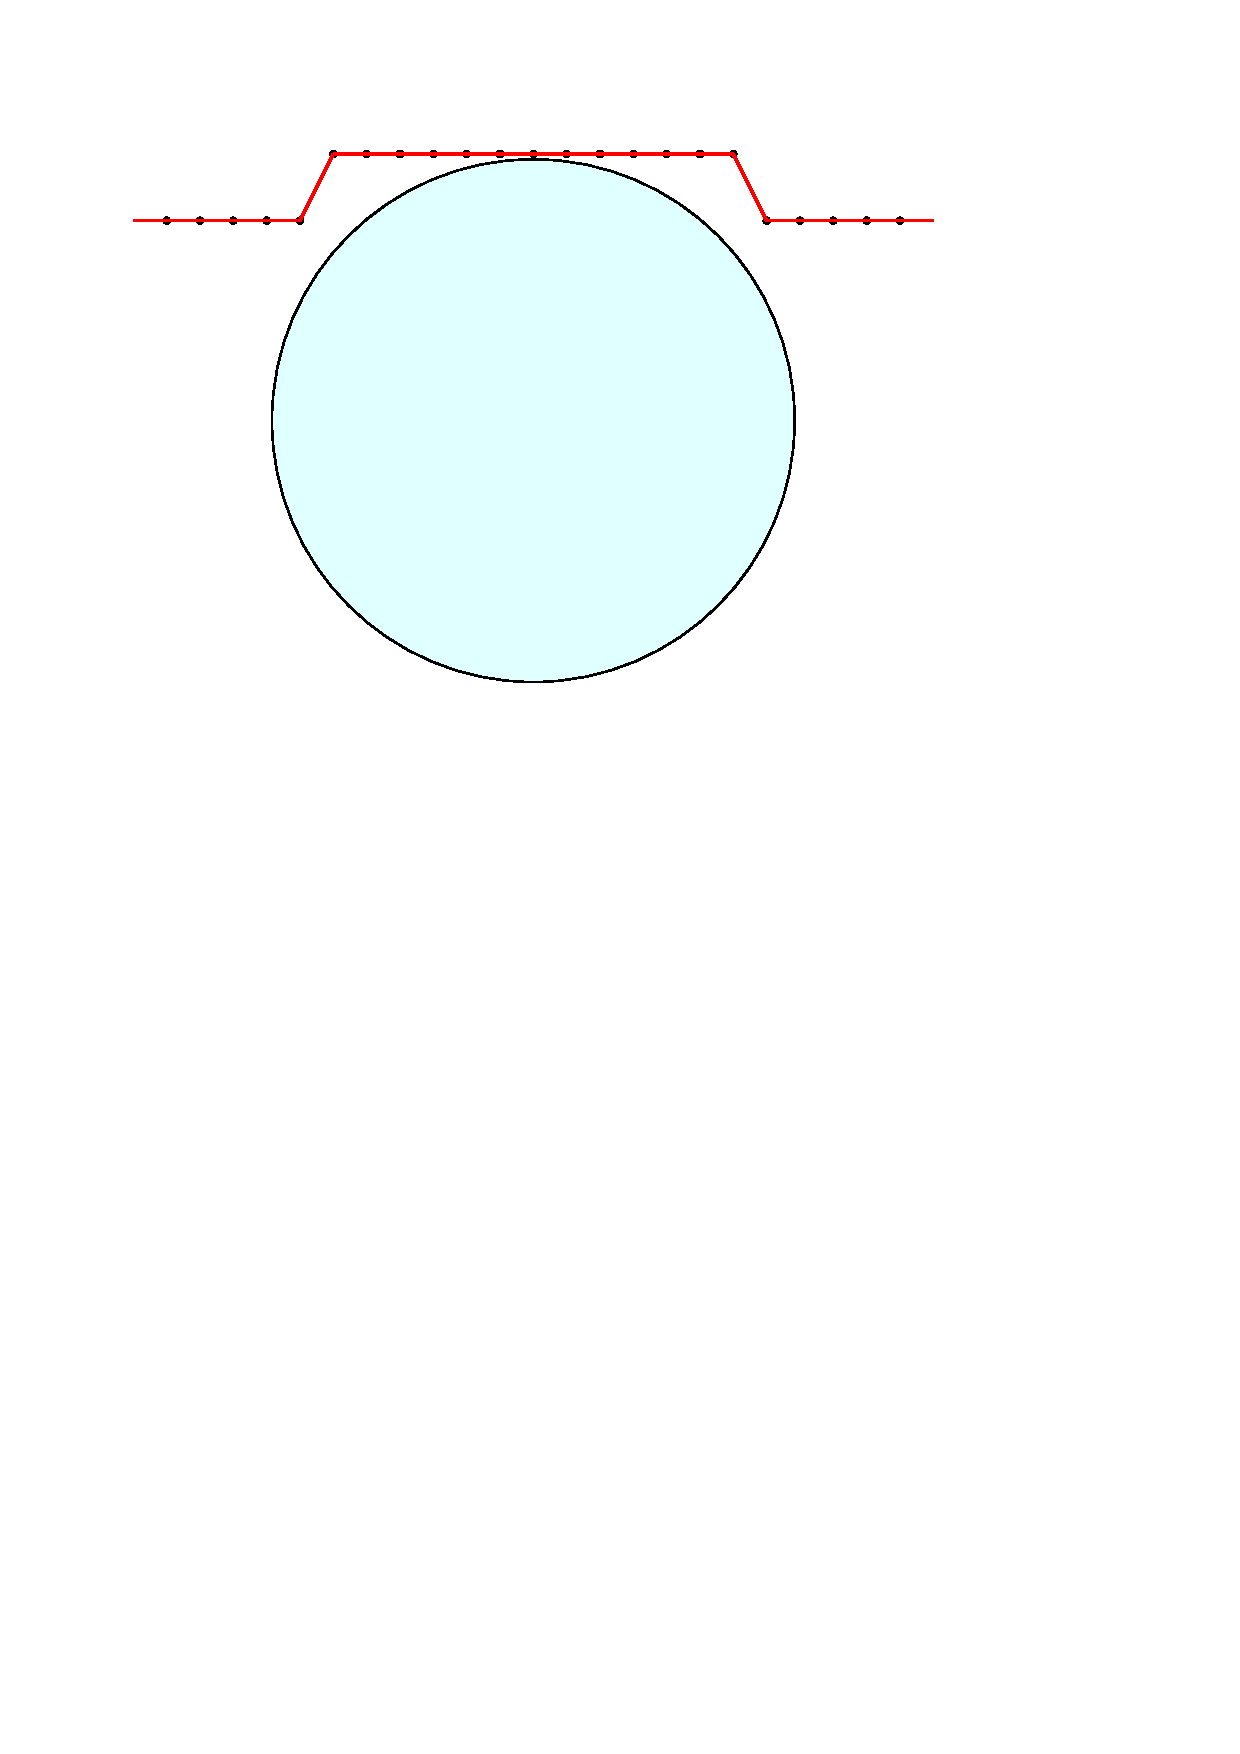
\includegraphics[width=\textwidth]{figures/collsn_demo_2}
	\caption{move back}
    \end{subfigure}
    \begin{subfigure}{0.48\columnwidth}
	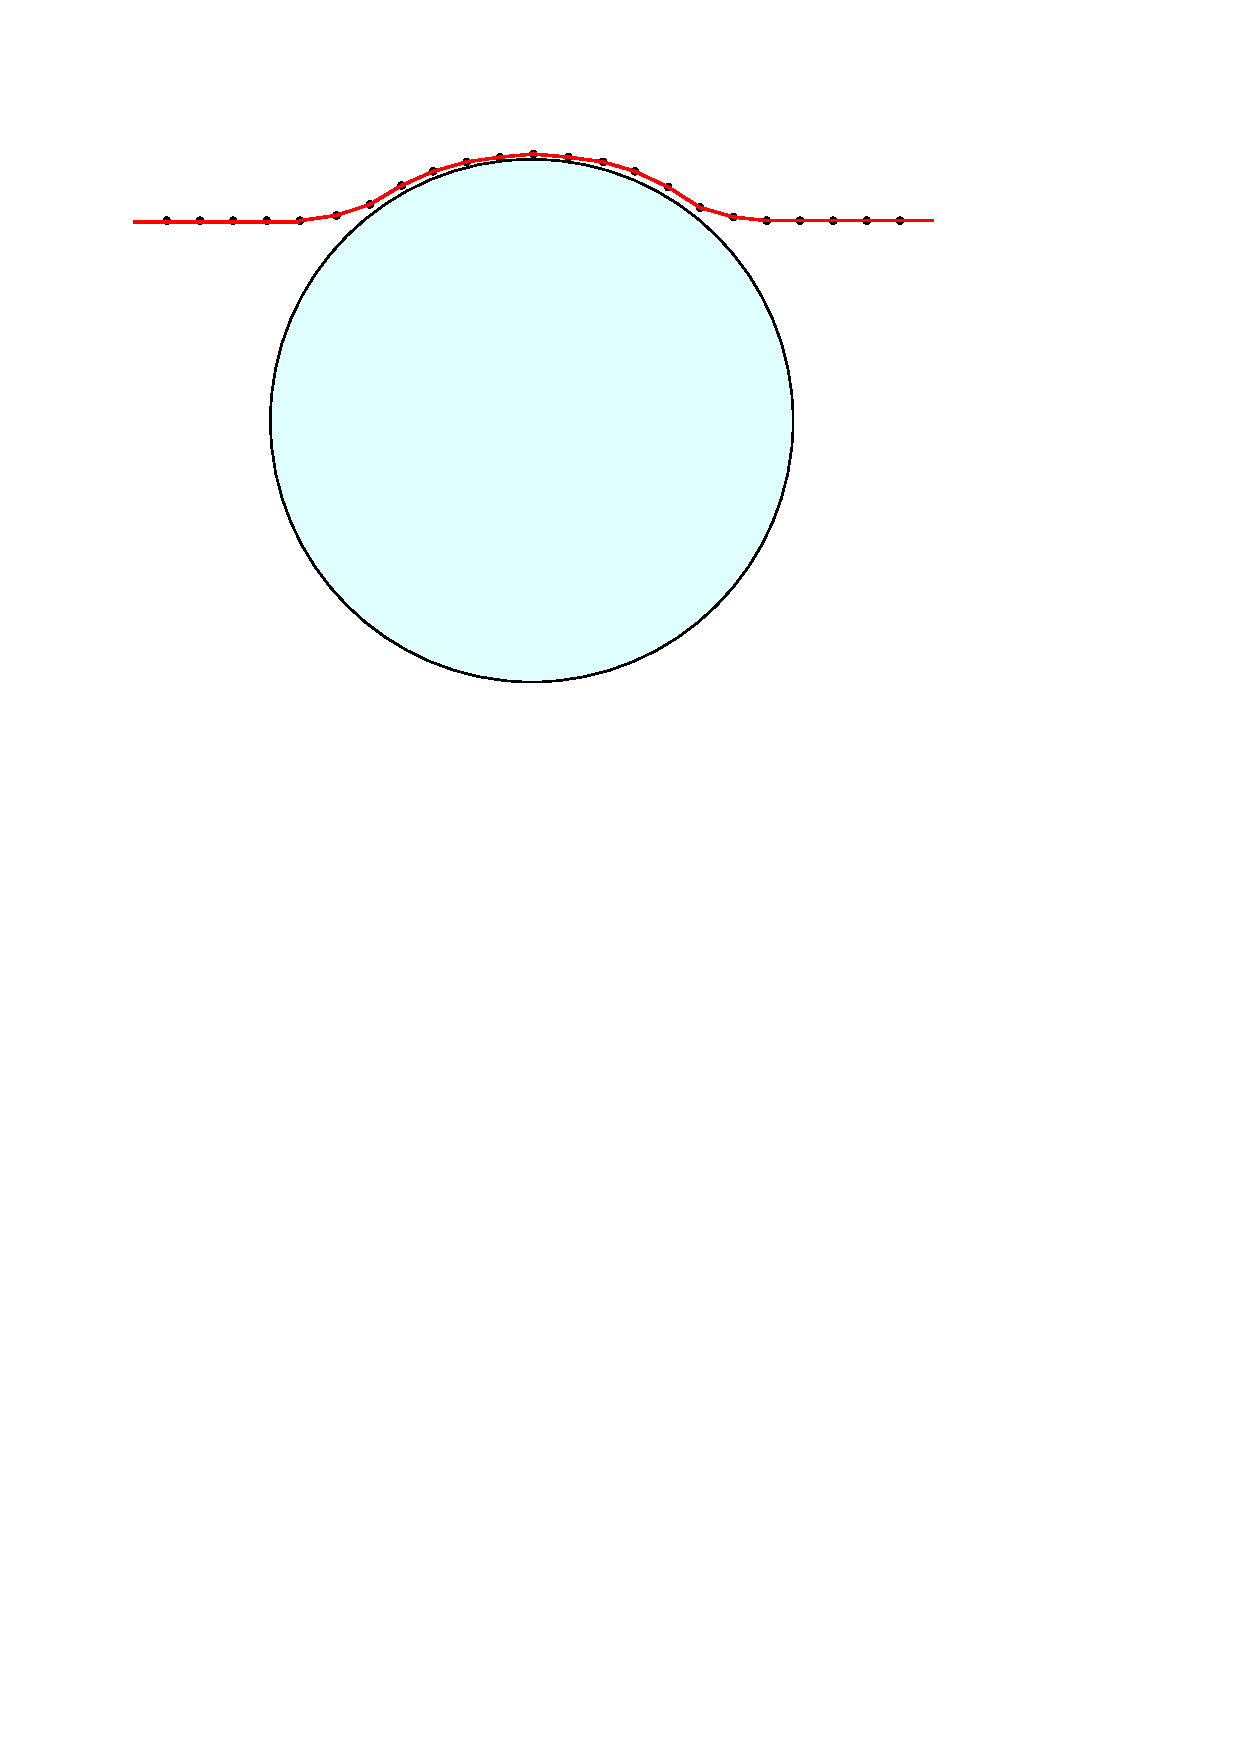
\includegraphics[width=\textwidth]{figures/collsn_demo_3}
	\caption{apply impulse}
    \end{subfigure}
    \caption{A demonstration of process how to resolve the collision. The red 
    line represents the fabric structure; the light-blue disk represents an 
    object; the points on the red line are the mass points in the spring 
    model.}
    \label{fig:collsn_demo}
\end{figure}

The following is a summary of the collision algorithm. The detection is
done by axis-aligned bounding box (AABB) tree, and the details of impulse
and impact zone technique are discussed in the following chapter.
\begin{itemize}
\item Pre-processing:
    \begin{itemize}
    \item Starting at $t^n$ with a time step $\Delta t$, record
    current positions $\mathbf{x}^{n}$ and velocities $\mathbf{v}^{n}$.
    \item Propagate all structures to the candidate positions
    $\mathbf{x}^{can}$ with candidate velocities
    $\mathbf{v}^{can}$ at time $t^{n+1}$, and compute the average velocity
    during this time step,
    $\mathbf{v}^{ave} = (\mathbf{x}^{can} - \mathbf{x}^{n}) / \Delta t$.
    \item Connect points on each rigid body (static or movable) as one
    impact zone.
    \end{itemize}
\item Detection and Handling:
    \begin{itemize}
    \item Perform the proximity check for $\mathbf{x}^{n}$ and apply
    impulse and friction to update $\mathbf{v}^{ave}$.
    \item Perform the collision check for propagation from $\mathbf{x}^{n}$
    with velocity $\mathbf{v}^{ave}$, and resolve collisions by applying
    impulse and rigid impact zones technique to update $\mathbf{v}^{ave}$.
    \item Update the candidate position of all the points by
    $\mathbf{x}^{can} = \mathbf{x}^{n} + \Delta t \mathbf{v}^{ave}$.
    \item If there is no more collision with respect to $\mathbf{x}^{can}$,
    continue to the post-processing; otherwise, repeat the detection and
    handling process.
    \end{itemize}
\item Post-processing:
    \begin{itemize}
    \item Advance the $\mathbf{v}^{ave}$ to $\mathbf{v}^{can}$ for points
    involved in collision, and, meanwhile, update the center of mass and
    center of mass velocity of the movable rigid bodies.
    \item Continue to the next time step with
    $\mathbf{x}^{n+1} = \mathbf{x}^{can}$ and
    $\mathbf{v}^{n+1} = \mathbf{v}^{can}$ for all points.
    \end{itemize}
\end{itemize}



\newpage
       % Mathematical Models
\chapter{Numerical Implementations}
\label{Chap:Numerical}

As mentioned earlier, the simulation of parachute system involves three 
major parts: computational structure dynamics, computational fluid 
dynamics and fluid-structure interaction. 
In this chapter, we discuss the detailed numerical methods for each part. 
The data structures and many functionalities are based on \FronTierp 
library developed for front tracking method \cite{GliGroLi99a,DuFixGli05}.



\section{ODE Solvers}
\label{Sec:ODES}

\subsection{Rigid Body Rotation}
As discussed in the \Sec{RGD}, the governed equations for rigid body 
rotation are \Eqn{eulers_equation2} which is an ODE system. 
We use the fourth-order Runge Kutta method, \Eqn{4th_RK}, to solve for the 
angular velocity $\mathbf{w}$. 
\begin{eqnarray}
\begin{aligned}
u^{n+1} &= u^{n} + h(k_{1} + 2k_{2} + 2k_{3} + k_{4})/6, \\
k_{1} &= \mathscr{L}(t_n, u^{n}), \\
k_{2} &= \mathscr{L}(t_n + h/2, u^{n} + hk_{1}/2), \\
k_{3} &= \mathscr{L}(t_n + h/2, u^{n} + hk_{2}/2), \\
k_{4} &= \mathscr{L}(t_n + h, u^{n} + hk_{3}),
\end{aligned}
\label{eqn:4th_RK}
\end{eqnarray}
where $h$ is the step size and $\mathscr{L}$ is a discretization spatial
operator.

The Euler angles ($\phi$, $\theta$, $\psi$) are visually straightforward.
However, they are difficult to use in numerical computation because of the
involve of trigonometric functions in the rotation matrix 
\Eqn{rotation_matrix1}, which could lead to singularity.
For numerical purpose, we use the four-parameter representation, Euler 
parameters $\mathbf{e} = (e_{0}, e_{1}, e_{2}, e_{3})$, for propagation 
of the rigid bodies, with the constraint \Eqn{Euler_params_constraint}. 
\begin{equation}
e_0^2 + e_1^2 + e_2^2 + e_3^2 = 1
\label{eqn:Euler_params_constraint}
\end{equation}

Euler's rotation theorem states that, in three-dimensional space, any 
displacement of a rigid body such taht a point on the rigid body remain 
fixed, is equivalend to a single rotation about some axis that runs 
through the fixed point. 
This fixed point can be considered as the rotation center. 
The Euler parameters are an interpretation of Euler's rotation theorem, which
is related to an angle of rotation $\alpha$ and a unit vector along the axis 
of rotation $\mathbf{u}$. 
\begin{eqnarray}
\begin{aligned}
e_0 &= \cos(\alpha / 2) \\
\left(
\begin{array}{c}
e_1 \\ e_2 \\ e_3 \\
\end{array}
\right) &= \mathbf{u} \sin(\alpha / 2)
\end{aligned}
\label{eqn:Euler_parameters}
\end{eqnarray}
The initial status means no rotation happens.
Therefore, initially, the Euler parameters are $\mathbf{e} = (1, 0, 0, 0)$.
The relationship between the Euler parameters $\mathbf{e}$ and the angular
velocity $\mathbf{w}$ is given by
\Eqn{euler_parameters_and_angular_velocity}. 
\begin{equation}
\left(
\begin{array}{c}
\dot{e}_0 \\ \dot{e}_1 \\ \dot{e}_2 \\ \dot{e}_3 \\
\end{array}
\right) = \frac{1}{2}
\left(
\begin{array}{ccc}
-e_1 & -e_2 & -e_3 \\
e_0 & e_3 & -e_2 \\
-e_3 & e_0 & e_1 \\
e_2 & -e_1 & e_0 \\
\end{array}
\right)
\left(
\begin{array}{c}
w_1 \\ w_2 \\ w_3 \\
\end{array}
\right)
\label{eqn:euler_parameters_and_angular_velocity}
\end{equation}
As well, fourth-order Runge Kutta method \Eqn{4th_RK} is applied.

Under this circumstance, the rotation matrix $A$ can be written in terms of 
the Euler parameters $\mathbf{e}$ as
\begin{equation}
A =\left(
\begin{array}{ccc}
e_0^2+e_1^2-e_2^2-e_3^2 & 2(e_1e_2+e_0e_3) & 2(e_1e_3-e_0e_2) \\
2(e_1e_2-e_0e_3) & e_0^2-e_1^2+e_2^2-e_3^2 & 2(e_2e_3+e_0e_1) \\
2(e_1e_3+e_0e_2) & 2(e_2e_3-e_0e_1) & e_0^2-e_1^2-e_2^2+e_3^2 \\
\end{array}
\right)
\label{eqn:rotation_matrix}
\end{equation}
The transpose $A^T$ is also the inverse of the rotation matrix $A$. 
$x' = Ax$ represents the rotation process from the world/space coordinates 
system to the body-fixed coordinates system, and $x = A^Tx'$ does the 
opposite process. 
Because the order of rotation in 3 dimensional cases matters, when 
propagating the rigid body from time $t_n$ to $t_{n+1}$, we have the 
following equation.
\begin{equation}
x_{n+1} = A^T_{n+1} A_n x_n
\end{equation}
The subscripts $n$ and $n+1$ are the time step index. This means we always 
first convert to the body-fixed coordinates system before apply the updated 
rotation matrix. 



\subsection{Spring Solver}
\label{Sec:SS}
For the spring-mass model, explicit integration with fourth order 
Runge-Kutta method \Eqn{4th_RK} is adopted to solve the ODE system 
\Eqn{sm_ODEs}.

The explicit scheme requires us to pay attention to the numerical stability 
of the spring solver. 
Based on the previous analysis and numerical verification in 
\cite{LiChernKimLi12, KimLiLi12}, the spring-mass system is a conservative 
system without external forces, and there exists an upper bound for the 
eigenfrequency of the oscillation 
\begin{equation}
w_{max} \leq \sqrt{\frac{2Mk}{m}}, 
\label{eqn:eigenfrequency}
\end{equation}
where $M$ is the maximum number of neighbors that a spring vertex has, $k$ 
is the tensile stiffness and $m$ is the point mass. 
The Delingette's modification adds variation to the spring model, but the 
upper bound is still valid except that the maximum tensile stiffness is used 
in \Eqn{eigenfrequency} instead. 
Therefore, for stability and accuracy purpose, we choose $w_{max}h < 0.1$ for 
simulations.



\section{PDE Solvers}
\label{Sec:PDES}

There have been many techniques to solve the governed equations that describes 
the motion of the fluid. 
For compressible fluid, \Eqn{Euler_eqns_con}, since it is a hyperbolic system, 
we apply the 5th Weighted Essentially Non-Oscillatory (WENO) scheme. 
For incompressible fluid, a pressure correction projection method is used, 
which can achieve second order accuracy. 

\subsection{WENO Scheme}
High-order numerical methods have been widely used to effectively resolve 
complex flow features such as turbulent or vertical flows 
\cite{Ekaterinaris2005192}. 
High-order shock-capturing schemes such as the Essentially Non-Oscillatory 
(ENO) and Weighted ENO (WENO) \cite{Liu1994200,Jiang1996202} schemes not 
only make the computational fluid dynamics (CFD) solvers get rid of 
extremely fine mesh for complex flows, but also perfectly eliminate the 
oscillations near discontinuities. 
WENO scheme is used to reconstruct the spatial derivative term and then the 
hyperbolic system is converted to an ODE system and propagated by 3rd order 
Total Variation Diminishing (TVD) Runge-Kutta method. 

Take one-dimensional Euler equation \Eqn{1d_Euler} for example
\begin{equation}
\mathbf{U}_{t}+\mathbf{F}\left(\mathbf{U}\right)_{x} = 0
\label{eqn:1d_Euler}
\end{equation}
where 
\begin{equation}
\mathbf{U} = 
\left(
\begin{array}{c}
\rho\\ \rho u\\ E
\end{array}
\right),\ 
\mathbf{F}(\mathbf{U}) = 
\left(
\begin{array}{c}
\rho u\\ \rho u^{2}+p\\ (E+p)u
\end{array}
\right)
\end{equation}
\begin{equation}
E = \rho (e+\frac{u^{2}}{2}),\ p = \rho e (\gamma - 1)
\end{equation}
$\rho$, $u$, $P$, $e$ and $\gamma$ denote the density, velocity,
pressure, internal energy per unit mass and ratio of specific heats,
respectively. The Jacobian matrix of the Euler equations is defined as 
\begin{equation}
\mathbf{A} = \frac{\partial \mathbf{F}(\mathbf{U})}{\partial \mathbf{U}}
\end{equation}
The eigenvalues of the Jacobian matrix $A$ are 
\begin{equation}
\lambda_{1} = u-c,\ \lambda_{2}=u,\ \lambda_{3}=u+c
\end{equation}
where $c=\sqrt{\frac{\gamma p}{\rho}}$ is the sound speed, and the
corresponding right eigenvectors are 
\begin{equation}
\mathbf{r}_{1} = 
\left(
\begin{array}{c}
1\\ u-a\\ H-ua
\end{array}
\right),\ 
\mathbf{r}_{2} = 
\left(
\begin{array}{c}
1\\ u\\ \frac{u^{2}}{2}
\end{array}
\right),\ 
\mathbf{r}_{3} = 
\left(
\begin{array}{c}
1\\ u + a\\ H + u a
\end{array}
\right)
\label{eqn:Euler_eigvec}
\end{equation}
where $H$ is the total specific enthalpy, which is related to the
specific enthalpy $h$ and other variables, namely 
\begin{equation}
H = \frac{E + p}{\rho} = \frac{1}{2}u^{2} + h,\ h = e + \frac{P}{\rho}
\end{equation}
We denote the matrix whose columns are eigenvectors in \Eqn{Euler_eigvec} by 
\begin{equation}
\mathbf{R} = \left(\mathbf{r}_{1},\mathbf{r}_{2},\mathbf{r}_{3}\right)
\end{equation}
and denote $\mathbf{L} = \mathbf{R}^{-1}$. The eigenvalue decomposition
of $\mathbf{A}$ is 
\begin{equation}
\mathbf{A} = \mathbf{R \Lambda L}
\end{equation}
where $\mathbf{\Lambda} = diag(u-c,u,u+c)$. Then, \Eqn{1d_Euler} can be 
transformed as 
\begin{equation}
\mathbf{(LU)}_{t} + \Lambda(\mathbf{LU})_{x} = 0
\label{eq:1d_transEuler}
\end{equation}
which consists of three independent one-dimensional hyperbolic equations. 
The advection term in each equation can be reconstructed using WENO scheme 
then solved by advection solver. 

\subsection{Projection Method}
Projection method is an effective way to numerically solve the time-dependent 
incompressible fluid flow problems. 
We apply the pressure-Poisson version of projection method 
\cite{Chorin68, KimMoin85, Brown2001accurate} is adopted to solve the 
Navier-Stokes \Eqn{navierstoke_eqns}. 
\begin{itemize}
\item step 1: Solve for the intermediate velocity $u^*$.
    \begin{eqnarray}
    \begin{aligned}
    \frac{u^* - u^n}{\Delta t} + \frac{1}{\rho} \nabla q &= -[(u \cdot \nabla) u]^{n + \frac{1}{2}} + \frac{\mu}{2\rho} \nabla^2 (u^* + u^n), \\
    B(u^{*}) &= 0, 
    \end{aligned}
    \label{eqn:projection_1}
    \end{eqnarray}
    where $q$ represents an approximation of $p^{n+\frac{1}{2}}$ and 
    $B(u^{*})$ is the boundary condition for $u^{*}$. 
    The term $[(u \cdot \nabla) u]^{n + \frac{1}{2}}$ represents an 
    approximation of the advection term, which is done by WENO scheme. 
    Crank-Nicolson scheme is used to solve this advection-diffusion equation. 
\item step 2: Perform the projection
    \begin{eqnarray}
    \begin{aligned}
    u^* &= u^{n+1} + \Delta t \nabla \phi^{n+1} \\
    \nabla \cdot u^{n+1} &= 0
    \end{aligned}
    \label{eqn:projection_2}
    \end{eqnarray}
    using the boundary conditions consistent with $B(u^{*}) = 0$ and 
    $u^{n+1}|_{\partial \Omega} = u^{n+1}_{b}$. 
    After elimimating $u^{n+1}$, the above two equation becomes a Poisson 
    equation of $\phi$ which is solved by iterative methods. 
\item step 3: Update the pressure.
    \begin{equation}
    p^{n+\frac{1}{2}} = q + \phi^{n+1} - \frac{\mu \Delta t}{2\rho} \nabla^2 \phi^{n+1}.
    \label{eqn:projection_3}
    \end{equation}
    The last term in the above equation gives the second-order accuracy. 
\end{itemize}



\section{Fluid-Structure Interaction}
\label{Sec:FSI}
The interaction between fluid and fabric surface structure is a crucial part 
of the parachute system simulation. 
As mentioned above, the canopy experiences three forces, the gravitational 
force due to the weight of the material, the fluid-generated force due to 
the pressure difference on two sides of the canopy, and the internal spring 
force (both restoring force and friction force). 

\subsection{Force Calculation}
We handle this by the impulse method \cite{KimLiLi12} on the \FronTierp 
platform. 
For each mass point in the spring system, we divide the impulse into three 
components, the gravitational impulse, the fluid impulse and the internal 
impulse due to the spring system, that is, 
\begin{equation}
\mathbf{I}_i^C = \mathbf{I}_{gi}^C + \mathbf{I}_{pi}^C + \mathbf{I}_{si}^C.
\end{equation}
Since no fluid interaction with the string chord is considered in our model, 
the impulse splitting for these mass points is 
\begin{equation}
\mathbf{I}_i^S = \mathbf{I}_{gi}^S + \mathbf{I}_{si}^S.
\end{equation}
The gravitational impulse is straightforward and has the same formula for 
the spring vertex on both the canopy and string chords. 
\begin{equation}
\mathbf{I}_{gi} = \int_{0}^{t} m_{i} \mathbf{g} ds.
\end{equation}
The fluid impulse is 
\begin{equation}
\mathbf{I}_{pi} = \int_{0}^{t} \sigma (p^{-} - p^{+}) \mathbf{n} ds, 
\end{equation}
where $\sigma$ is the mass density of canopy per unity area, $p^{-}$ and 
$p^{+}$ are the pressure on the lower side and upper side of the canopy, 
and $n$ is the unit normal vector pointing from lower to upper side of the 
canopy. 
This follows \cite{Kalro00} for its simplicity. 
A more accurate calculation should also include the velocity shear near the 
canopy surface and stress to the surface. 

For the calculation of the reacting impulse between the canopy and the 
fluid, we apply the immersed boundary method which treats the reaction of 
the canopy as the normal force approximated by the smoothed delta function, 
that is Peskin's delta function, 
\begin{equation}
\mathbf{f}(\mathbf{x}, t) = \int \mathbf{F}(\mathbf{x}, t) \delta(x - \mathbf{X}(s, t)) ds.
\label{eqn:peskin_delta}
\end{equation}
The difference is that we use the impulse of the mass point as a result 
of the superposition of three forces from the spring system, 
\begin{equation}
\mathbf{F}(\mathbf{x}_{i}, t) = d(\mathbf{I}_{g} + \mathbf{I}_{p} + \mathbf{I}_{s}) / dt.
\end{equation}
Numerically, the surface force is the product of the normal component of 
the acceleration and mass density at the canopy surface 
\begin{equation}
\mathbf{F}(s, t) = \rho_{c} (\mathbf{a} \cdot \mathbf{n}) \mathbf{n}, 
\end{equation}
where $\mathbf{n}$ is the unit normal vector on the canopy surface, and 
$\rho_{c}$ is the mass density of canopy per unit area.

\subsection{Local Index Coating}
Our simulation of the parachute system is performed on the \FronTierp 
platform, which uses the front tracking method. 
This method is widely used for tracing the fluid interface in multi-phase 
flow problems, such as the Rayleigh-Taylor instability 
\cite{GliMcBMen86, GliLiMen90}, Richtmyer–Meshkov instability 
\cite{GarGliGro88}, and the jet problems \cite{GliKim04, GliLiOh02}. 
In problems like these, the fluid interface is topologically a manifold, 
the two sides of each surface are the boundaries of two separate domains. 
However, it is not the case in the simulation of parachute system where 
the canopy surface is thinness and forms an open boundary. 
You cannot tell which side of the canopy surface it belongs when a point is 
far away from it. 
But, for points that are sufficiently close to the canopy surface, we can 
still distinguish which side it belongs. 

The reason that we pay attention to this is that the local side information 
of space points that are near the canopy surface contributes to the 
calculation of the pressure difference, and thus the fluid force on the 
canopy. 
The pressure on two sides of the canopy surface is not continuous and it 
should be interpolated using the pressure information on its own side, which 
is realized by locally mesh coating algorithm.
Assign the domain in which the canopy is immersed with index $l$, and the 
local index coating algorithm follows three steps: 
\begin{itemize}
\item For any grid point $P$ with a distance $d \leq h$ away from the canopy, 
where $h$ is the grid spacing, find the nearest point on the canopy surface 
(\FronTierp is well equipped with these geometry functions) $P_{s}$. 
Using the sign of the scalar product $\overline{PP_{s}} \cdot \mathbf{n}_{s}$, 
we can determine the side of the point. 
Reassign domain index to $l-1$ if the point $P$ is on the negative side, 
otherwise reassign the index to $l+1$.
\item Reassign any grid point adjacent to a point indexed $l-1$ to the same; 
reassign any grid point adjacent to a point indexed $l+1$ to the same. 
Repeat this assignment for three sweeps. 
The resulting landscape of the grid index will look like \Fig{local_coating}. 
\item The interpolation of side-sensitive variables will use grid points of 
the same locally coated index.
\end{itemize}
\begin{figure}[!ht]
\centering
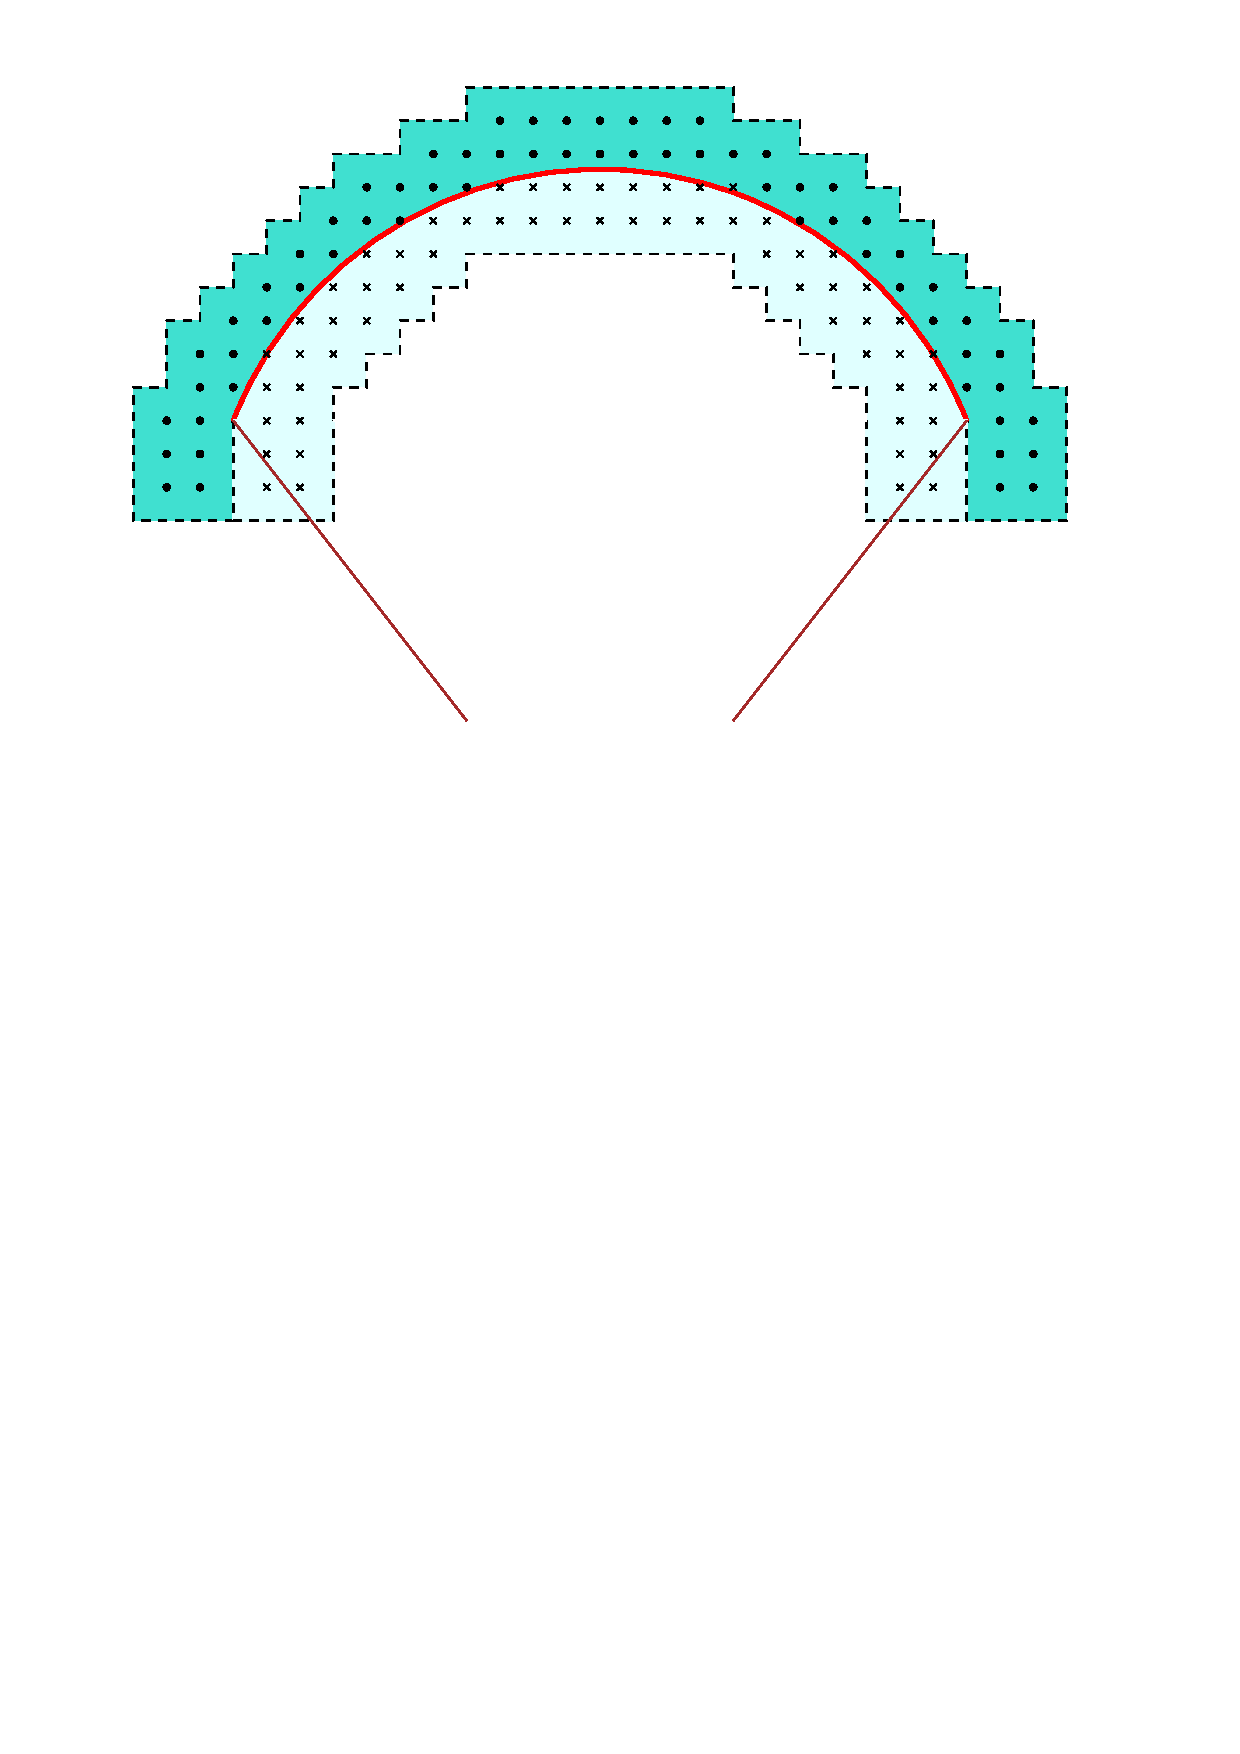
\includegraphics[width=0.7\columnwidth]{figures/local_coating}
\caption{The parachute canopy is an open surface and cannot separate the 
space into sub-domains. But we can still coat different index for mesh 
cells close to the surface using the local geometrical information. The 
light and dark shaded polygons represent the sets of mesh cells on the 
positive and negative sides of the canopy, respectively. An interpolation 
is carried out on vertex of the same color.}
\label{fig:local_coating}
\end{figure}



\section{Collision Features}
\label{Sec:CF}
Collision module for structures is a new feature added to the computational
framework.
With triangulized meshes, the proximity and collision checks can be broken
down into two major cases: a point against a triangle, an edge against
another edge.
For example, when there is collision detected between a pair of triangles,
15 tests need to be done in total.
\begin{itemize}
\item each point of one triangle against the other triangle
\item each edge of one triangle against each edge of the other triangle
\end{itemize}
When strings are taken into account, the comparison pairs can be not only
triangle-triangle, but also edge-edge and edge-triangle, because a string is
represented by a group of connected edges.
Similarly, there is 1 check for a edge-edge pair, and 5 checks for a
edge-triangle pair.

When there are movable rigid bodies involved in collision, we make use of the
impact zone technique which is first proposed in \cite{Provot1997} and further
developed in \cite{Bridson2002collsn}.
This technique was initially proposed to deal with multiple collisions and
maintain collision consistency.
The idea of the impact zone technique is to collect the points in multiple
collisions into separated zones, and treat them as rigid bodies.
Therefore, we can construct each movable rigid body as one independent impact
zone before resolving collisions.
Similar handling as cloth is applied to movable rigid bodies, but we adopted
some differences.
\begin{itemize}
\item The impulse added to each mass point due to collision consists of two
components: inelastic impulse and elastic impulse.
    \begin{itemize}
    \item If the two structures that collid are the same type, i.e. two
    elastic structures or two rigid structures, the inelastic impulse is
    distributed according to the mass
    \begin{equation}
    I_{in, i} = m_{1}m_{2}v_{n} / (m_1 + m_2); 
    \end{equation}
    otherwise, it is distributed evenly
    \begin{equation}
    I_{in,i} = 0.5 m_{i}v_{n}. 
    \end{equation}
    In above, $m_{1}$ and $m_{2}$ are masses and $v_{n}$ is the magnitude of
    relative velocity in the normal direction.
    \item When there is elastic structure(s) involved in the collision,
    the elastic impulse performs like a repulsion due to the elasticity
    \begin{equation}
    I_{el, i} = -min(\Delta t k d, m_{i}(0.1d/\Delta t - v_{n})); 
    \end{equation}
    otherwise, it is the case of two rigid structures
    \begin{equation}
    I_{el, i} = cr I_{in, i}. 
    \end{equation}
    Here, $d$ is the overlap length, $k$ is the string stiffness and $cr$ is
    the restitution coefficient.
    \end{itemize}
\item Whenever an impulse acts on some point on a movable rigid body, it is
spread, via impact zone connection, to all the points on that rigid body.
This is the constraint to maintain the geometric shape of the rigid bodies.
\item The impulse due to cloth-involved collision and that due to rigid
collision are recorded and averaged separately.
Because there will be much more collision detected with cloth, while fewer
between rigid bodies.
\end{itemize}



\newpage
   % Numerical Methods
\chapter{Numerical Results}

\section{Rigid Body in Fluid Flow}

\subsection*{Compressible Fluid}

\subsection*{Incompressible Fluid}



\section{Parachute System Simulation}
With our spring-mass model and the numerical methods mentioned above, we can
simulate different types of parachute on \FronTierp platform.
\Fig{canopies} shows three types of parachute canopy after fully
inflated due to the interaction from the inflow air.
\begin{figure}[!ht]
\centering
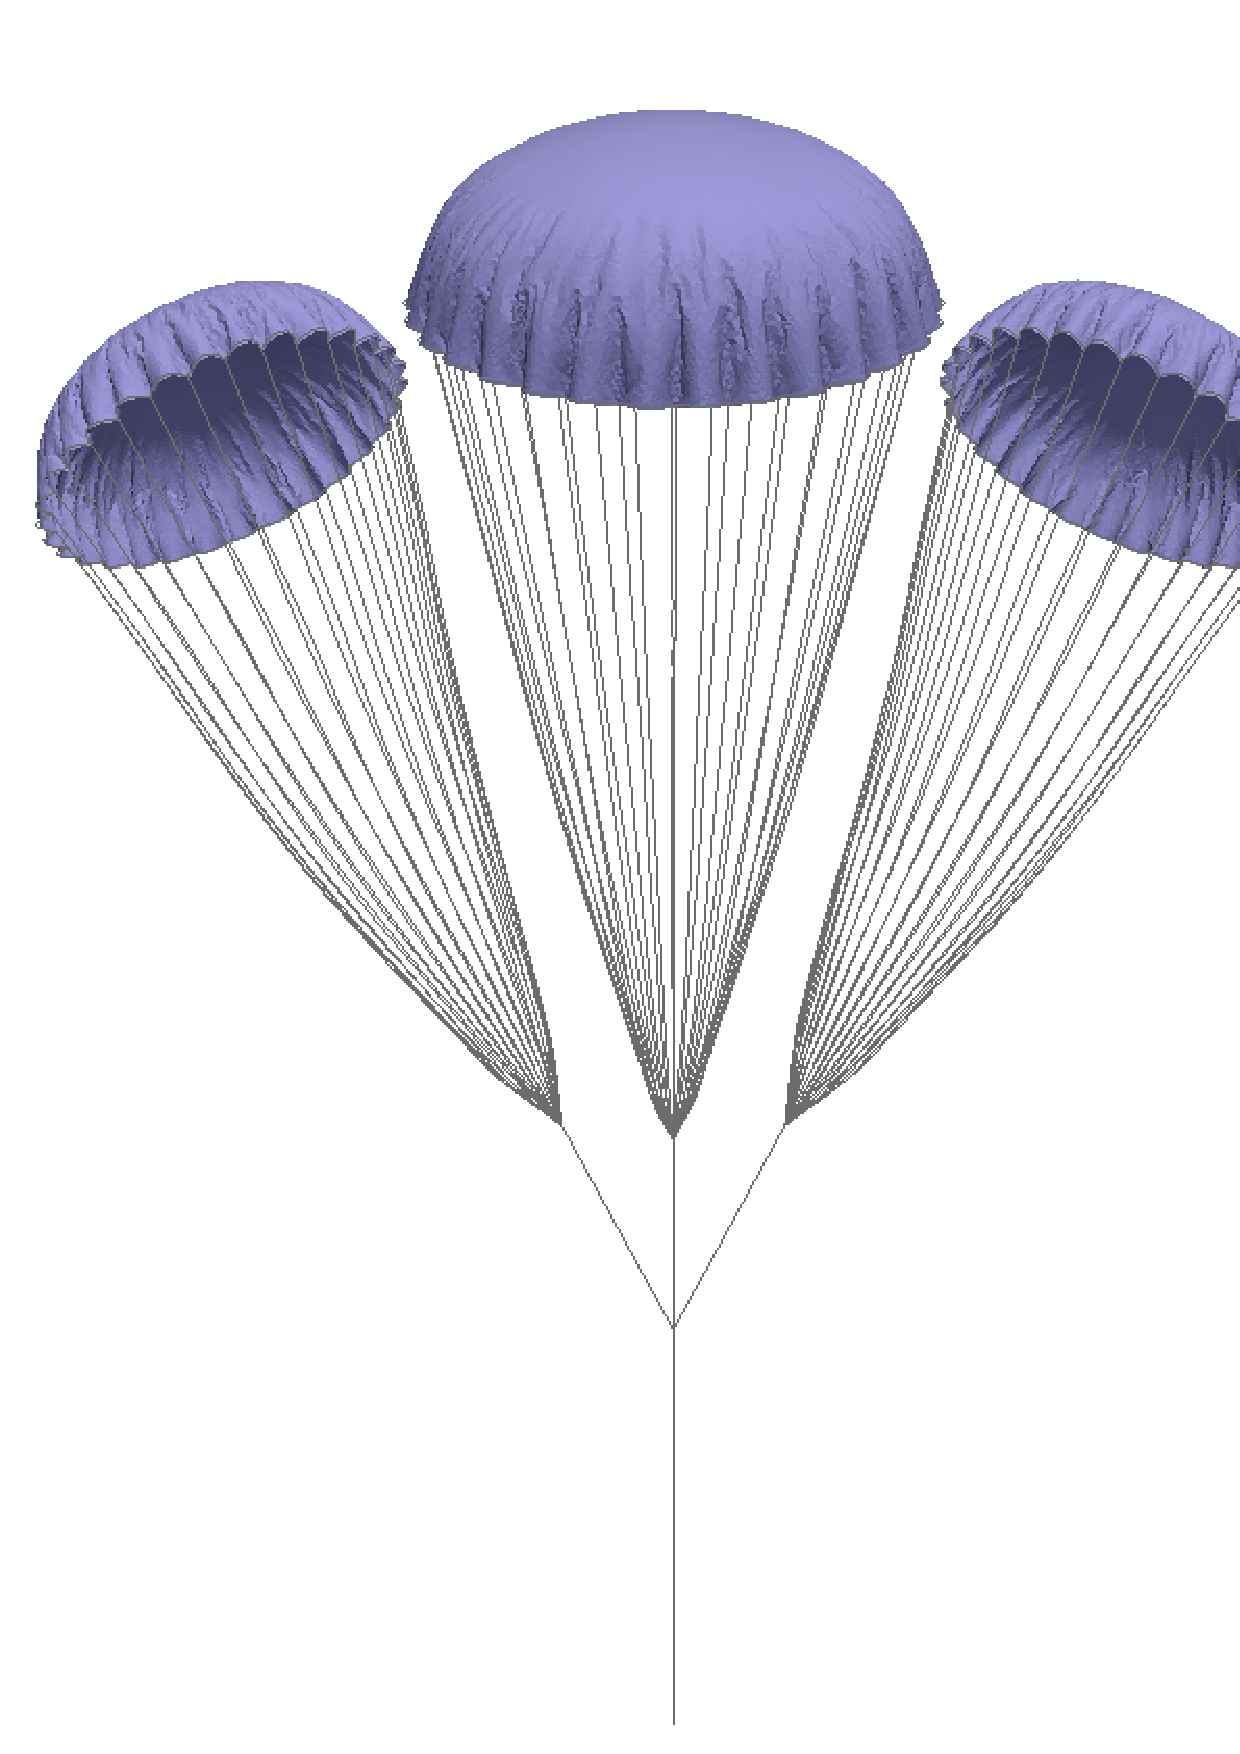
\includegraphics[width=0.32\textwidth]{figures/3G11_canopy}
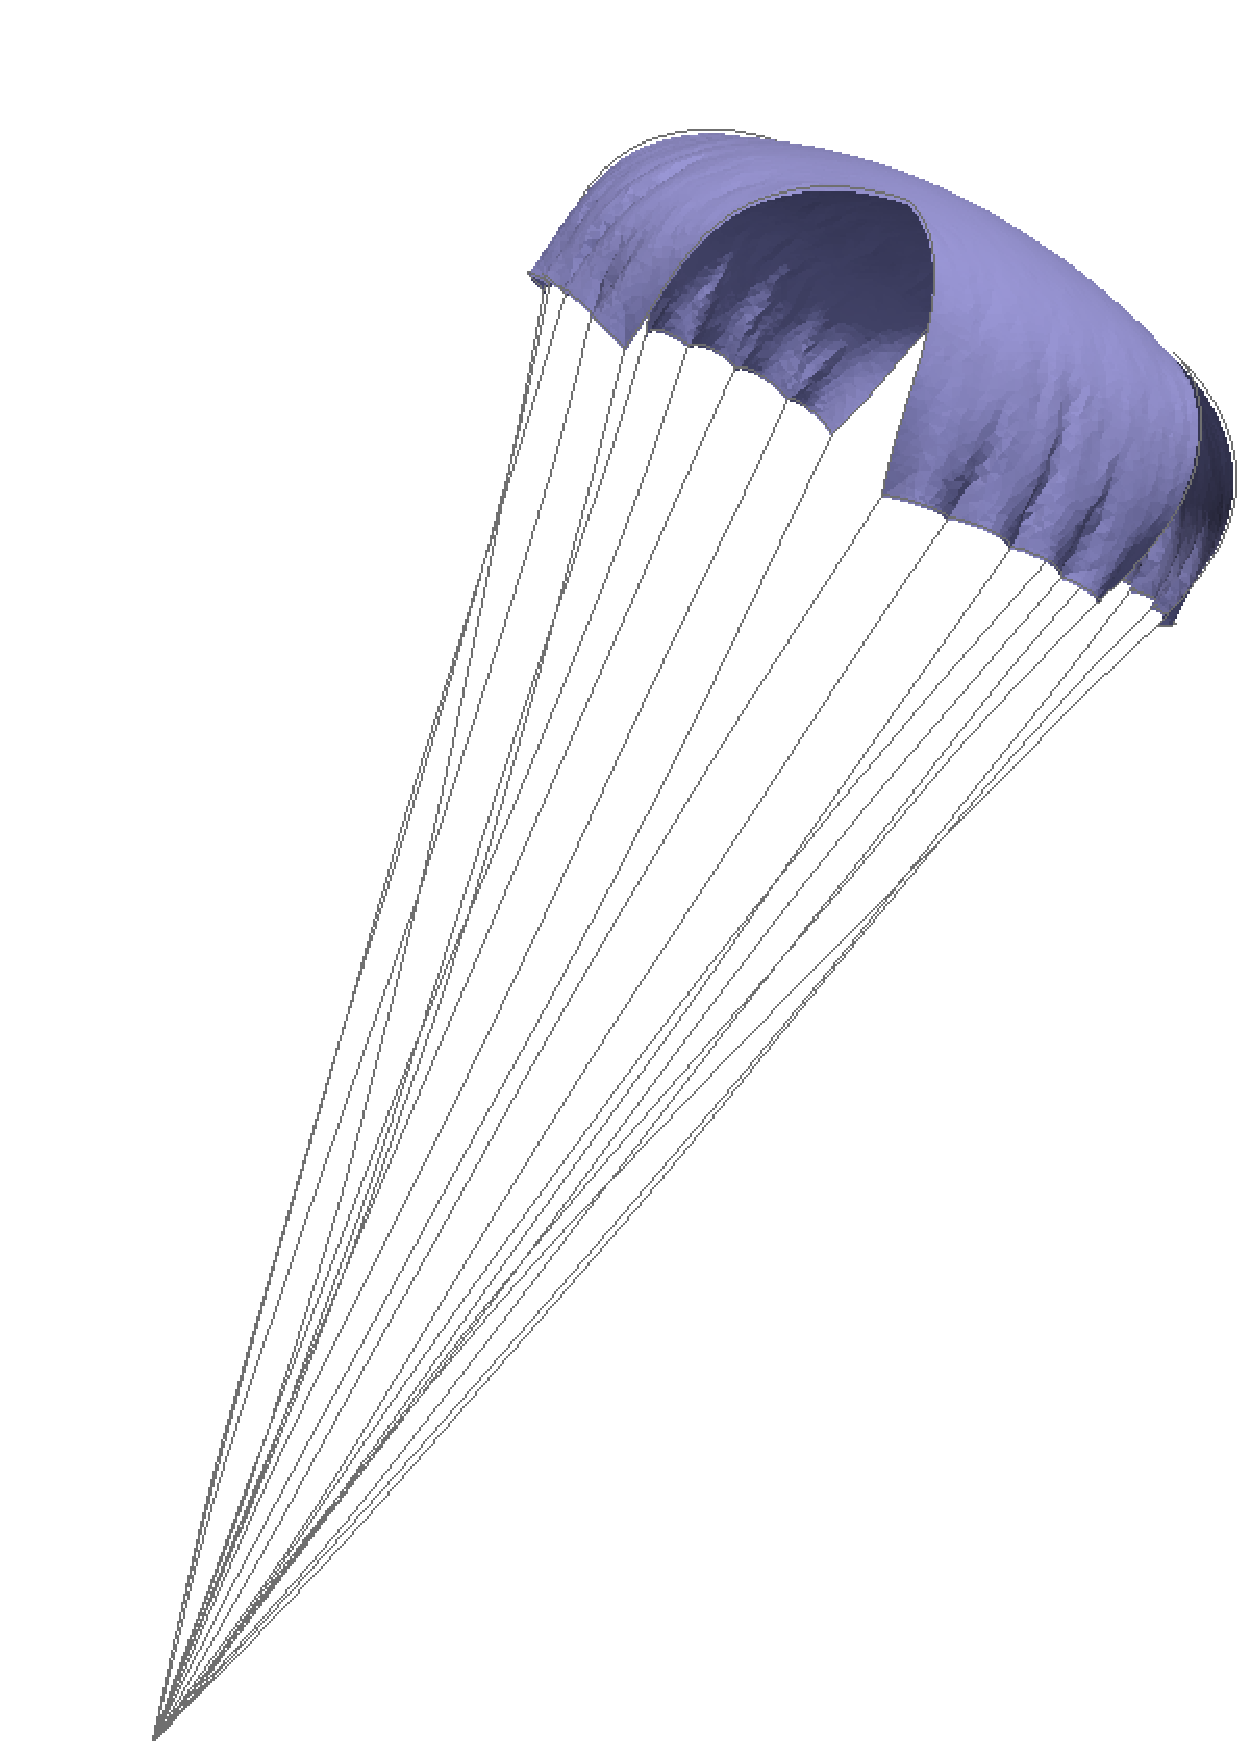
\includegraphics[width=0.32\textwidth]{figures/Cross_canopy}
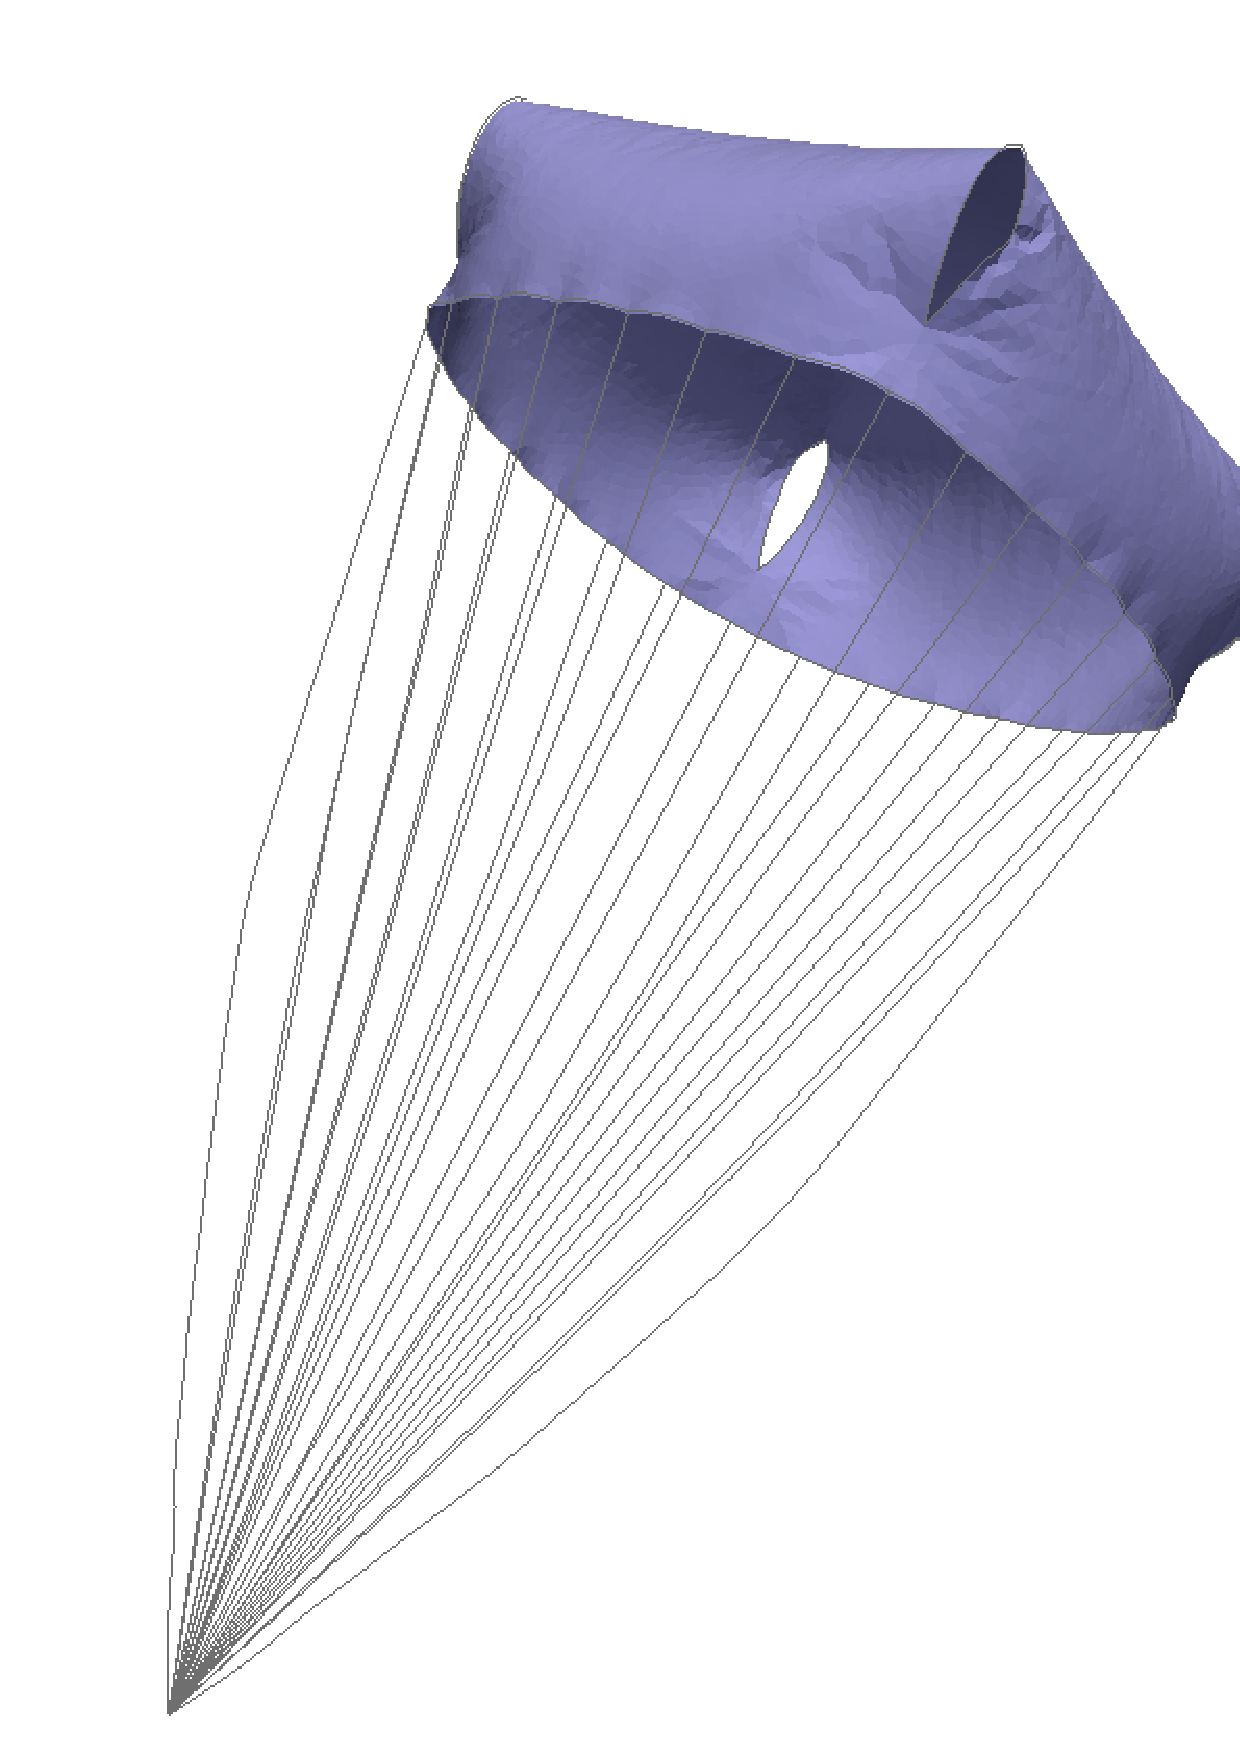
\includegraphics[width=0.32\textwidth]{figures/T11_canopy}
\caption{Three different types of parachute canopies simulated in \FronTierp
with our spring-mass model. Given parameters of a parachute, such as shape,
size, number of chords, \FronTierp has the capability to generate it.}
\label{fig:canopies}
\end{figure}

\subsection{Parachue Inflation}
Parachute inflation process is one of the most crucial stages for the
deceleration system.
In \Fig{C9_vort}, the cross-sectional velocity profile is  demonstrated at
different stages.
In this simulation, a C-9 personnel parachute with its nominal diameter
$8.53 m$ is taken as an example, and the computational domain is
$16 m\times16 m\times36 m$ with constant upward inflow velocity, outflow
boundary condition at upper outlet with pressure $p = 0$ and periodic
boundaries at the rest faces.
\begin{figure*}
\centering
\includegraphics[width=1\textwidth]{figures/C9_vort}
\caption{The cross-sectional velocity profiles around C-9 personnel
parachute during the falling process, at time $t = 1.2 s$, $t = 2.0 s$
and $t = 3.2 s$, respectively. In each plot, the left half shows the
velocity direction by arrow and the right half shows the velocity
magnitude by color, where red is large and blue is small.}
\label{fig:C9_vort}
\end{figure*}

\subsection{Wake of Parachutist}
Coupled with spring model explained in the previous sub-sections, we 
demonstrate the effect caused by the weak of the parachutist taking the 
C-9 personnel parachute (without vent) with its nominal diameter $8.53 m$ 
as an example, and set the computational domain to be 
$16 m\times16 m\times36 m$ with constant upward inflow velocity, outflow 
boundary condition at upper outlet with pressure $p = 0$ and periodic 
boundaries at the rest faces.
\begin{figure}[!ht]
\centering
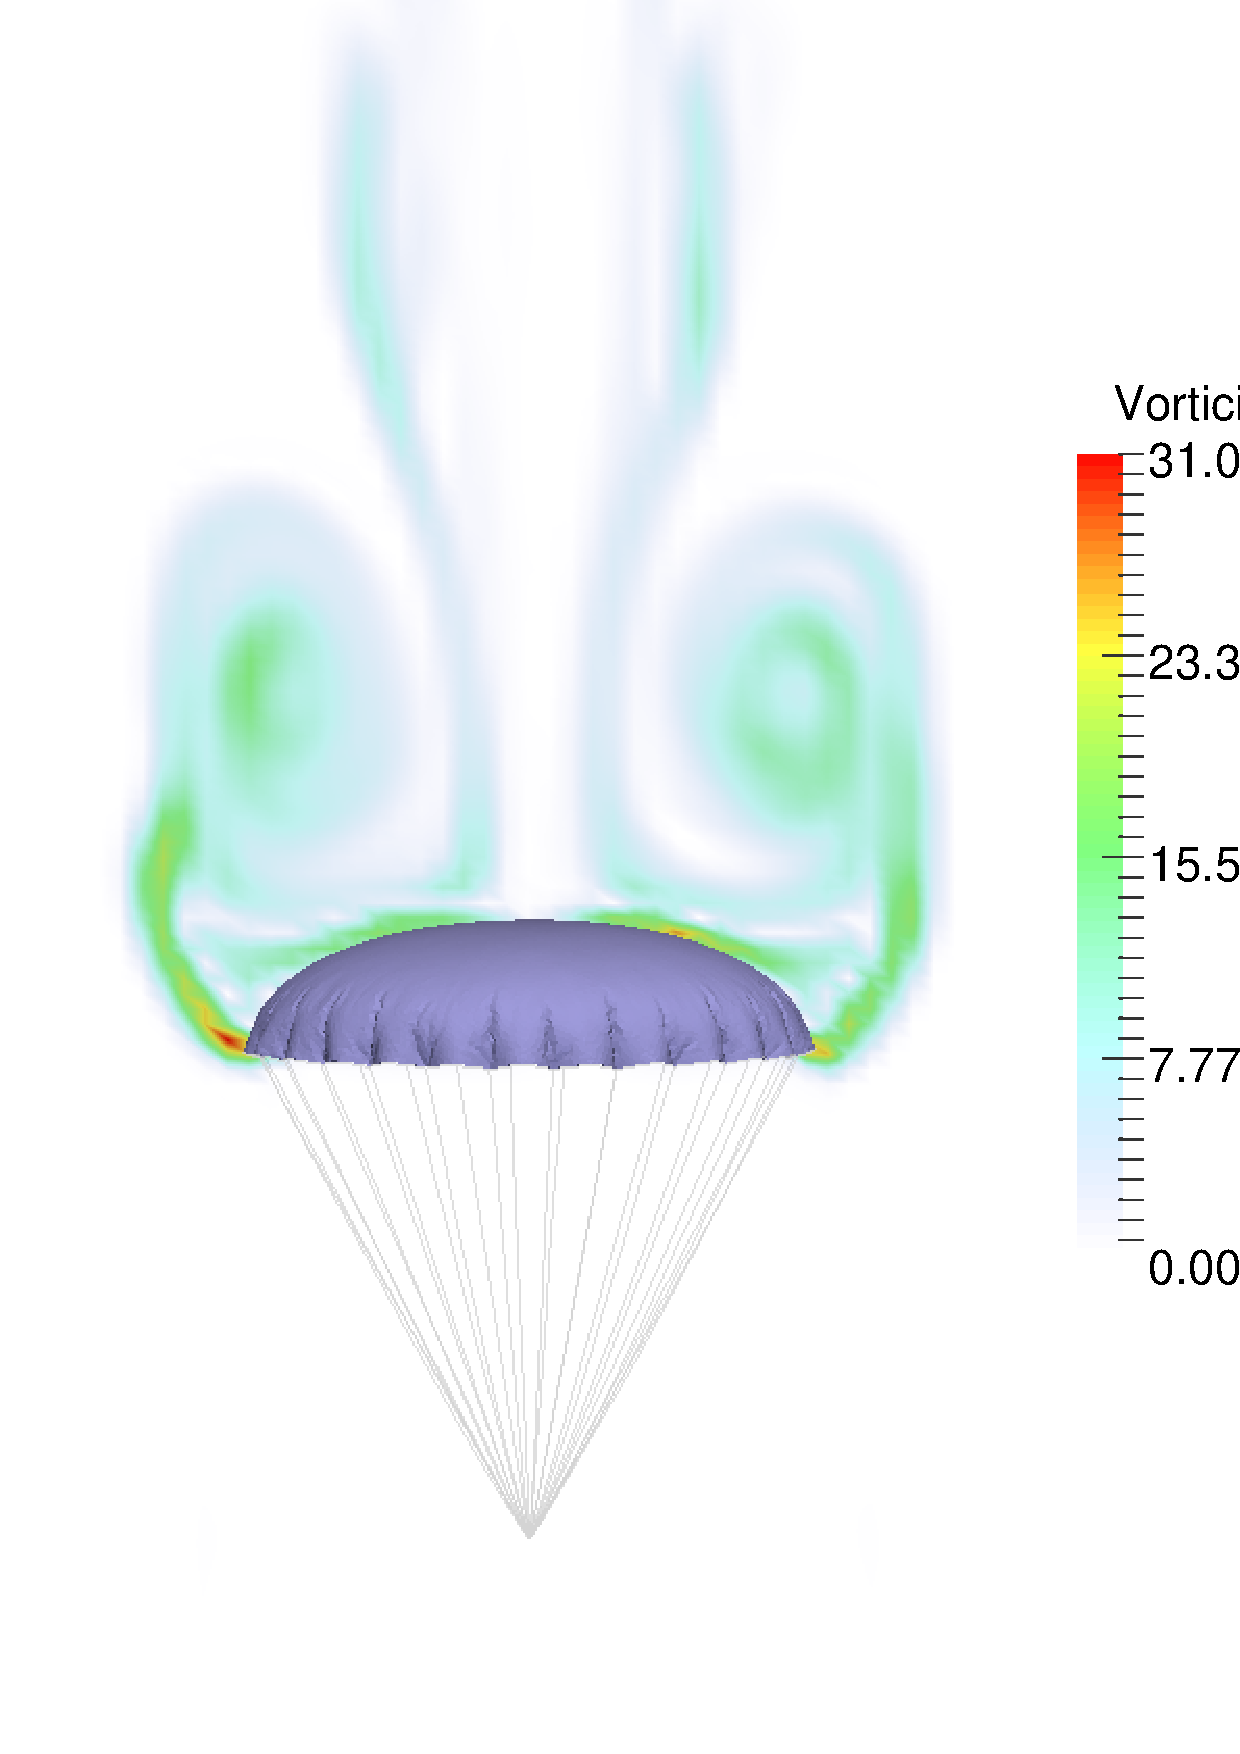
\includegraphics[width=0.48\columnwidth]{figures/C9_nohuman_vort}
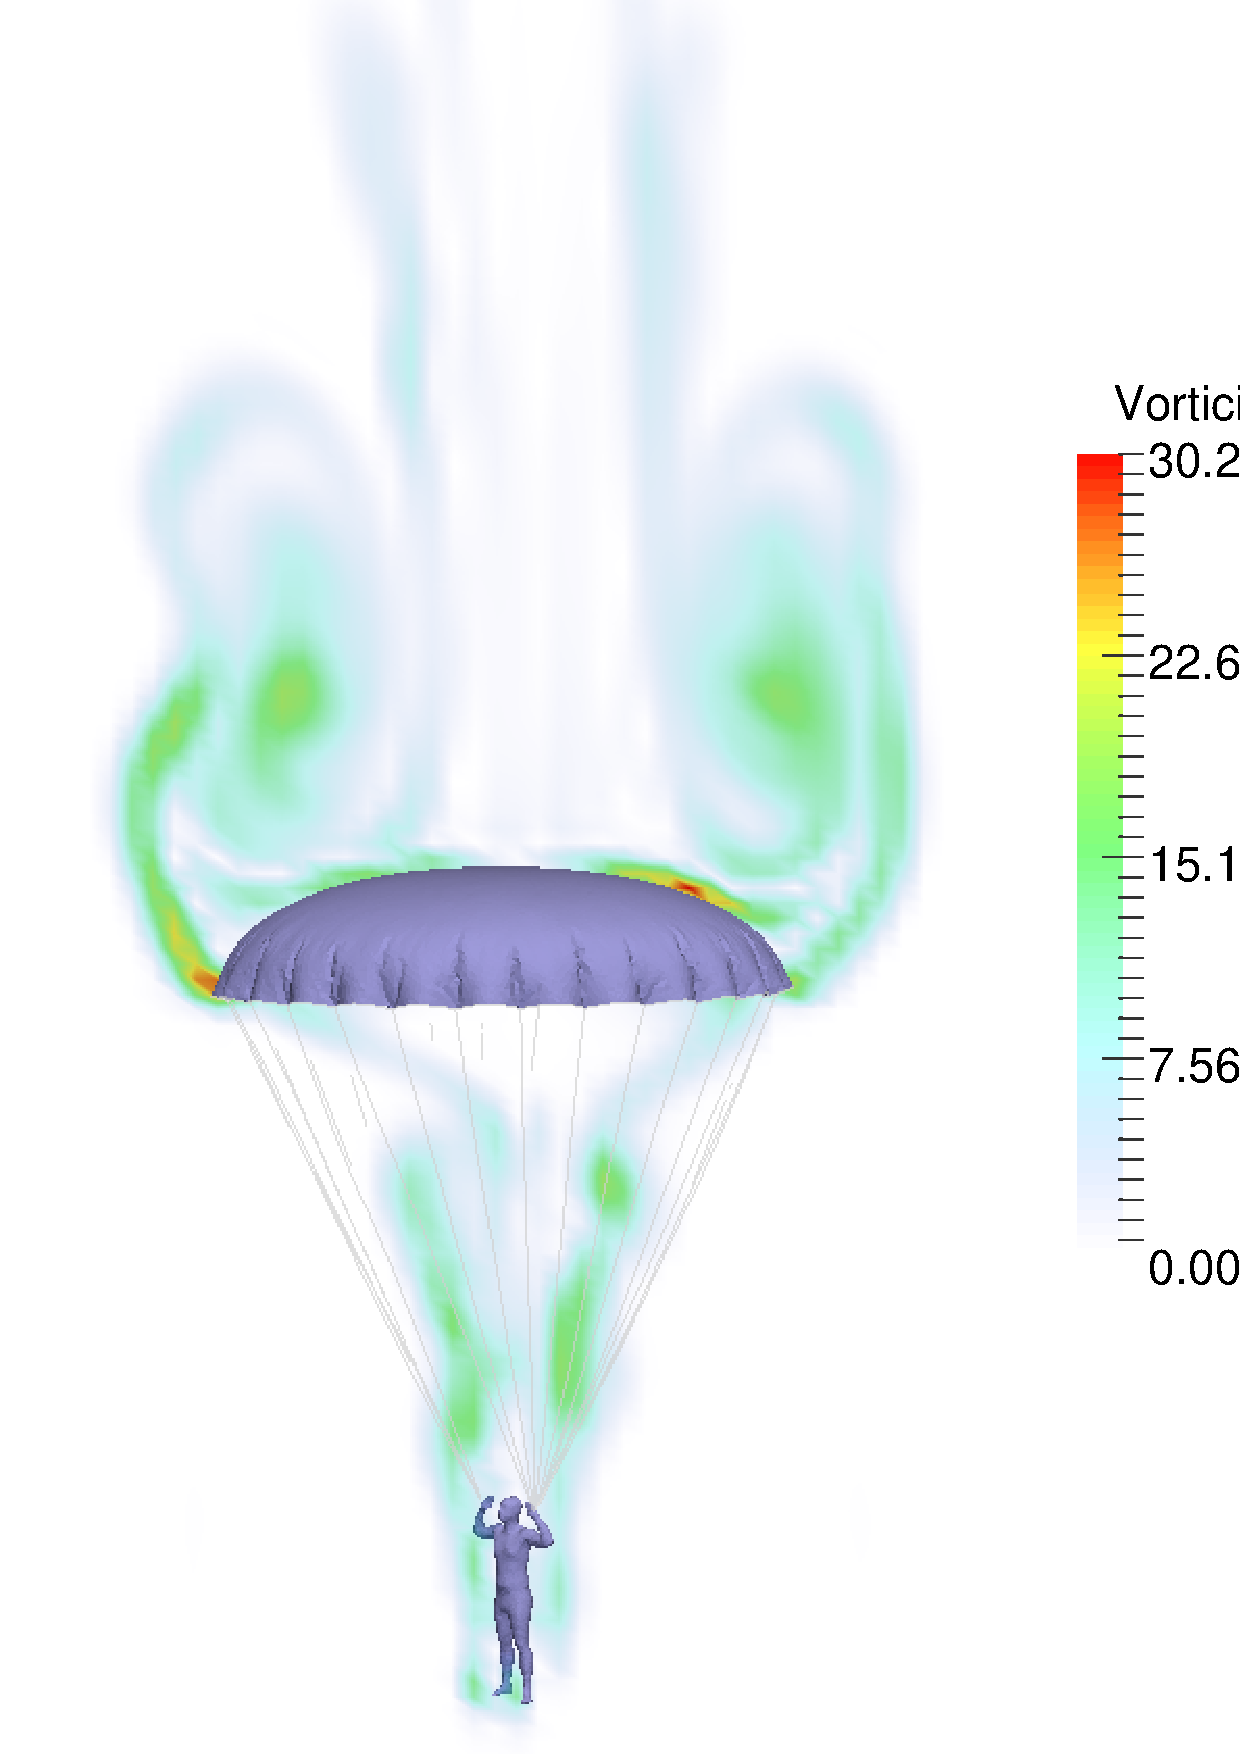
\includegraphics[width=0.48\columnwidth]{figures/C9_human_vort}
\caption{Comparison of the cross-sectional vorticity magnitude field. 
In the left figure, the parachutist is a mass point, while in the right 
figure, it is a rigid body with finite volume.}
\label{fig:C9_compare}
\end{figure}

Observed from \Fig{C9_compare}, there is turbulent flow as 
expected when the fluid flow passes the parachutist. 
Besides, the descent speed of the parachutist is slightly smaller when it is considered as a rigid body with finite volume. 
This is due to the interaction between the parachutist and the fluid flow, 
which generate an upward external force on it. 
Meanwhile, when the turbulent flow generated from fluid passing the 
parachutist reaches the canopy surface, it also has an upward force on the 
parachute system, and thus, reduces the descent speed.

\subsection{Uneven/Breaking Strings}
When designing a parachute, it is undesirable to have uneven suspension
lines or have some suspension lines broken at some time.
Here, we demonstrate these two cases in a wind tunnle test on a C-9 personnel
parachute with the computational domain size $12 m\times12 m\times24 m$.
The boundary conditions are set to be the same as above.
\begin{figure}[!ht]
\centering
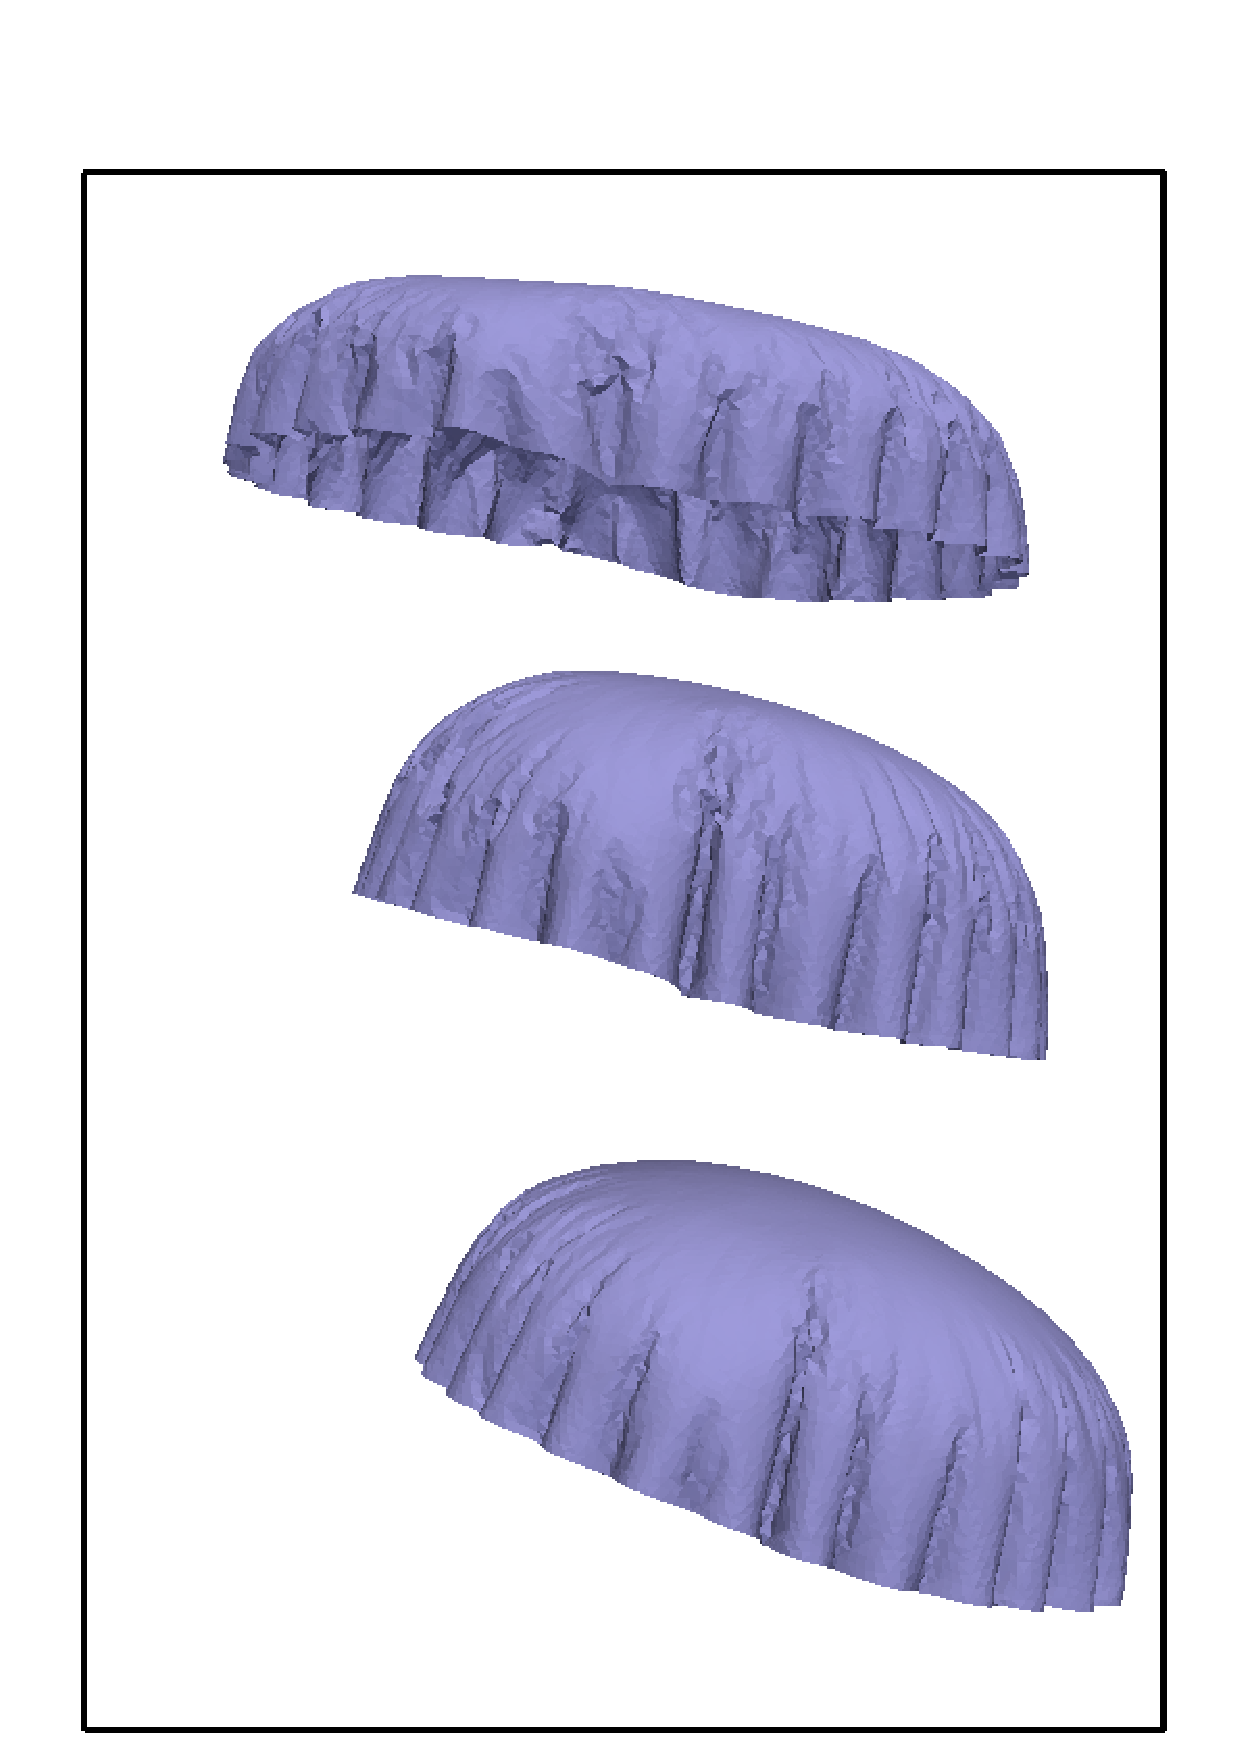
\includegraphics[width=0.48\textwidth]{figures/uneven}
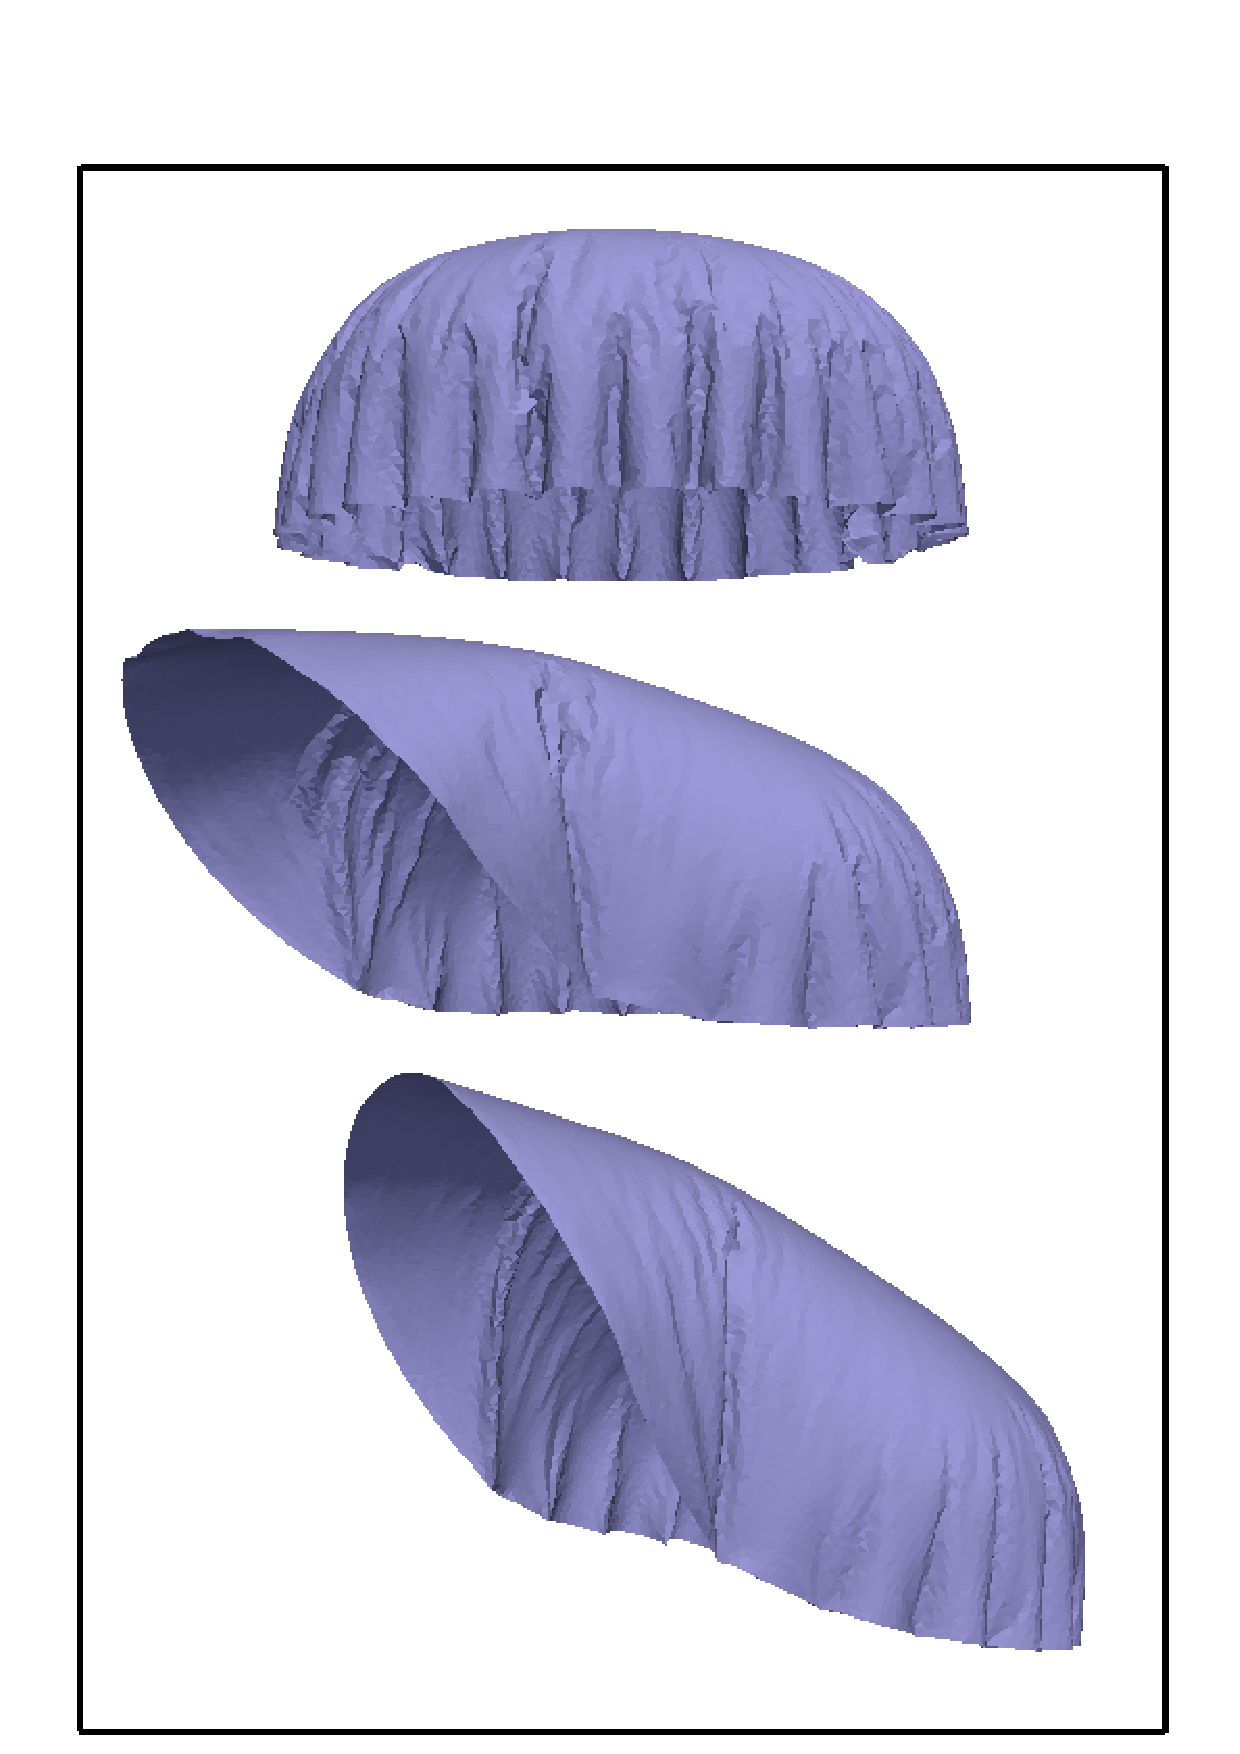
\includegraphics[width=0.48\textwidth]{figures/break}
\caption{The canopy surface of the C-9 personnel parachute at different time.
Left: 10 suspension lines are selected to have an equilibrium length than
others. Right: 10 suspension lines are selected to break at time $t = 5.0s$.}
\label{fig:uneven_break}
\end{figure}
In the left plot of \Fig{uneven_break}, 10 of the suspension lines have an
equibluim length $0.3 m$ shorter than normal which is $7 m$; while in the
right plot of \Fig{uneven_break}, 10 selected suspension lines break at
$t = 5.0s$.
Easy to observe that both cases cause the parachute canopy surface to be
unstable and lead to an angled deployment.
If the angle is too large, it could be dangerous.



\section{Collision Simulations}
As mentioned in the previous chapters, the algorithm is extended to
work for rigid bodies as well.
Since it is difficult to evaluate the correctness of cloth collision, we pay
more attention to the robustness of the algorithm.

\subsection{Benchmark: Rigid Bodies}
Because one-dimensional collisions between rigid bodies can be analytically
solved from the macro-aspect and have closed formula for velocities, we can
use this test case to demonstrate the correctness of the algorithm.
The closed formula is given by
\begin{equation}
\begin{aligned}
\widetilde{v}_a &= \frac{C_R m_b(v_b-v_a)+m_a v_a+m_b v_b}{m_a+m_b} \\
\widetilde{v}_b &= \frac{C_R m_a(v_a-v_b)+m_a v_a+m_b v_b}{m_a+m_b}
\end{aligned}
\label{eqn:rg_collsn_velo}
\end{equation}
where $C_R$ is the coefficient of restitution.
It is 1 for a complete elastic collision, and 0 for complete inelastic
collision.

Consider two cuboids initially moving toward each with velocity 0.5$m/s$ and
-0.5$m/s$ in $x$ direction, and the masses are 1$kg$ and 2$kg$, respectively.
Using formula \Eqn{rg_collsn_velo}, the speed after collision is
\begin{equation}
\begin{aligned}
\widetilde{v}_a &= -\frac{1}{6} m/s,\ 
\widetilde{v}_b = -\frac{1}{6} m/s, \mbox{ with $C_R = 0$}; \\
\widetilde{v}_a &= -\frac{5}{6} m/s,\ 
\widetilde{v}_b = \frac{1}{6} m/s,\ \mbox{ with $C_R = 1$}.
\end{aligned}
\end{equation}

\begin{figure}[!ht]
\centering
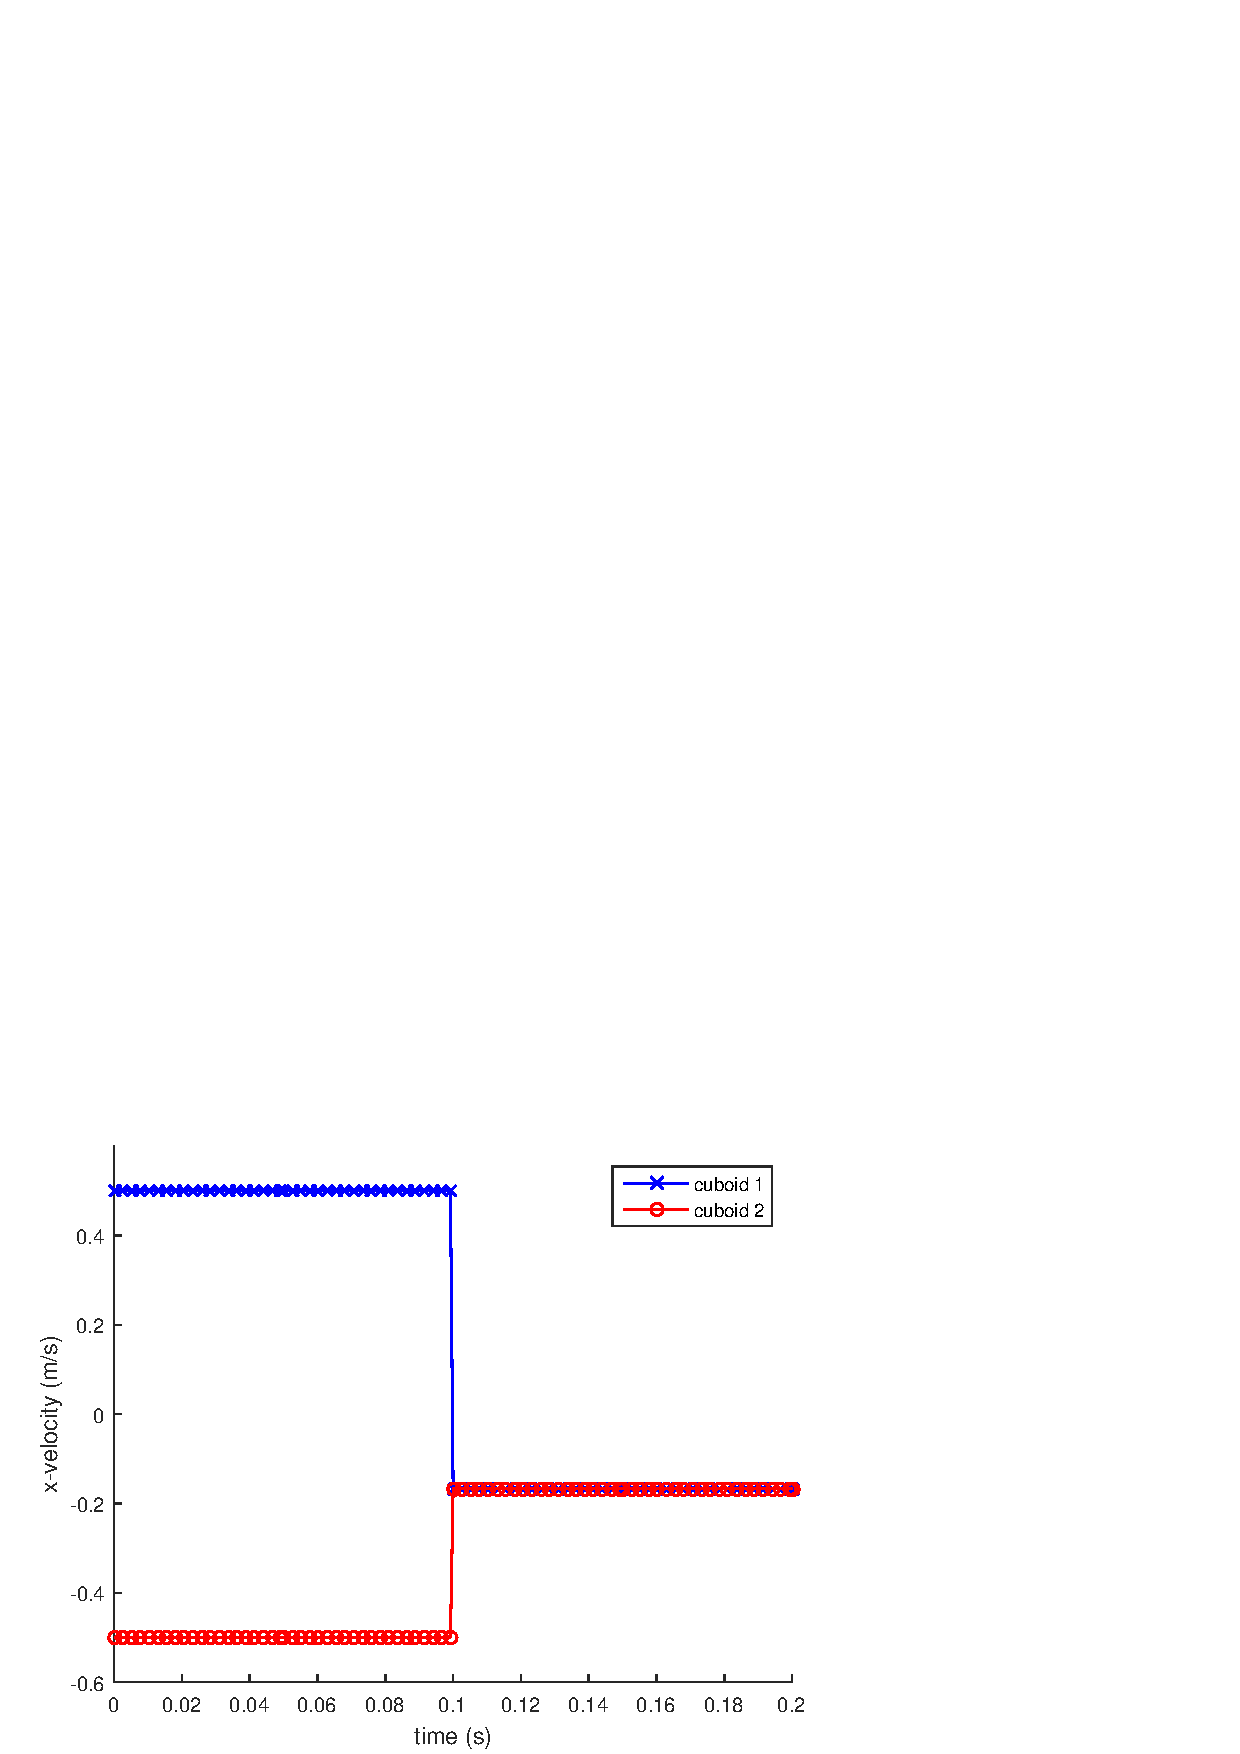
\includegraphics[width=0.48\textwidth]{figures/inelastic}
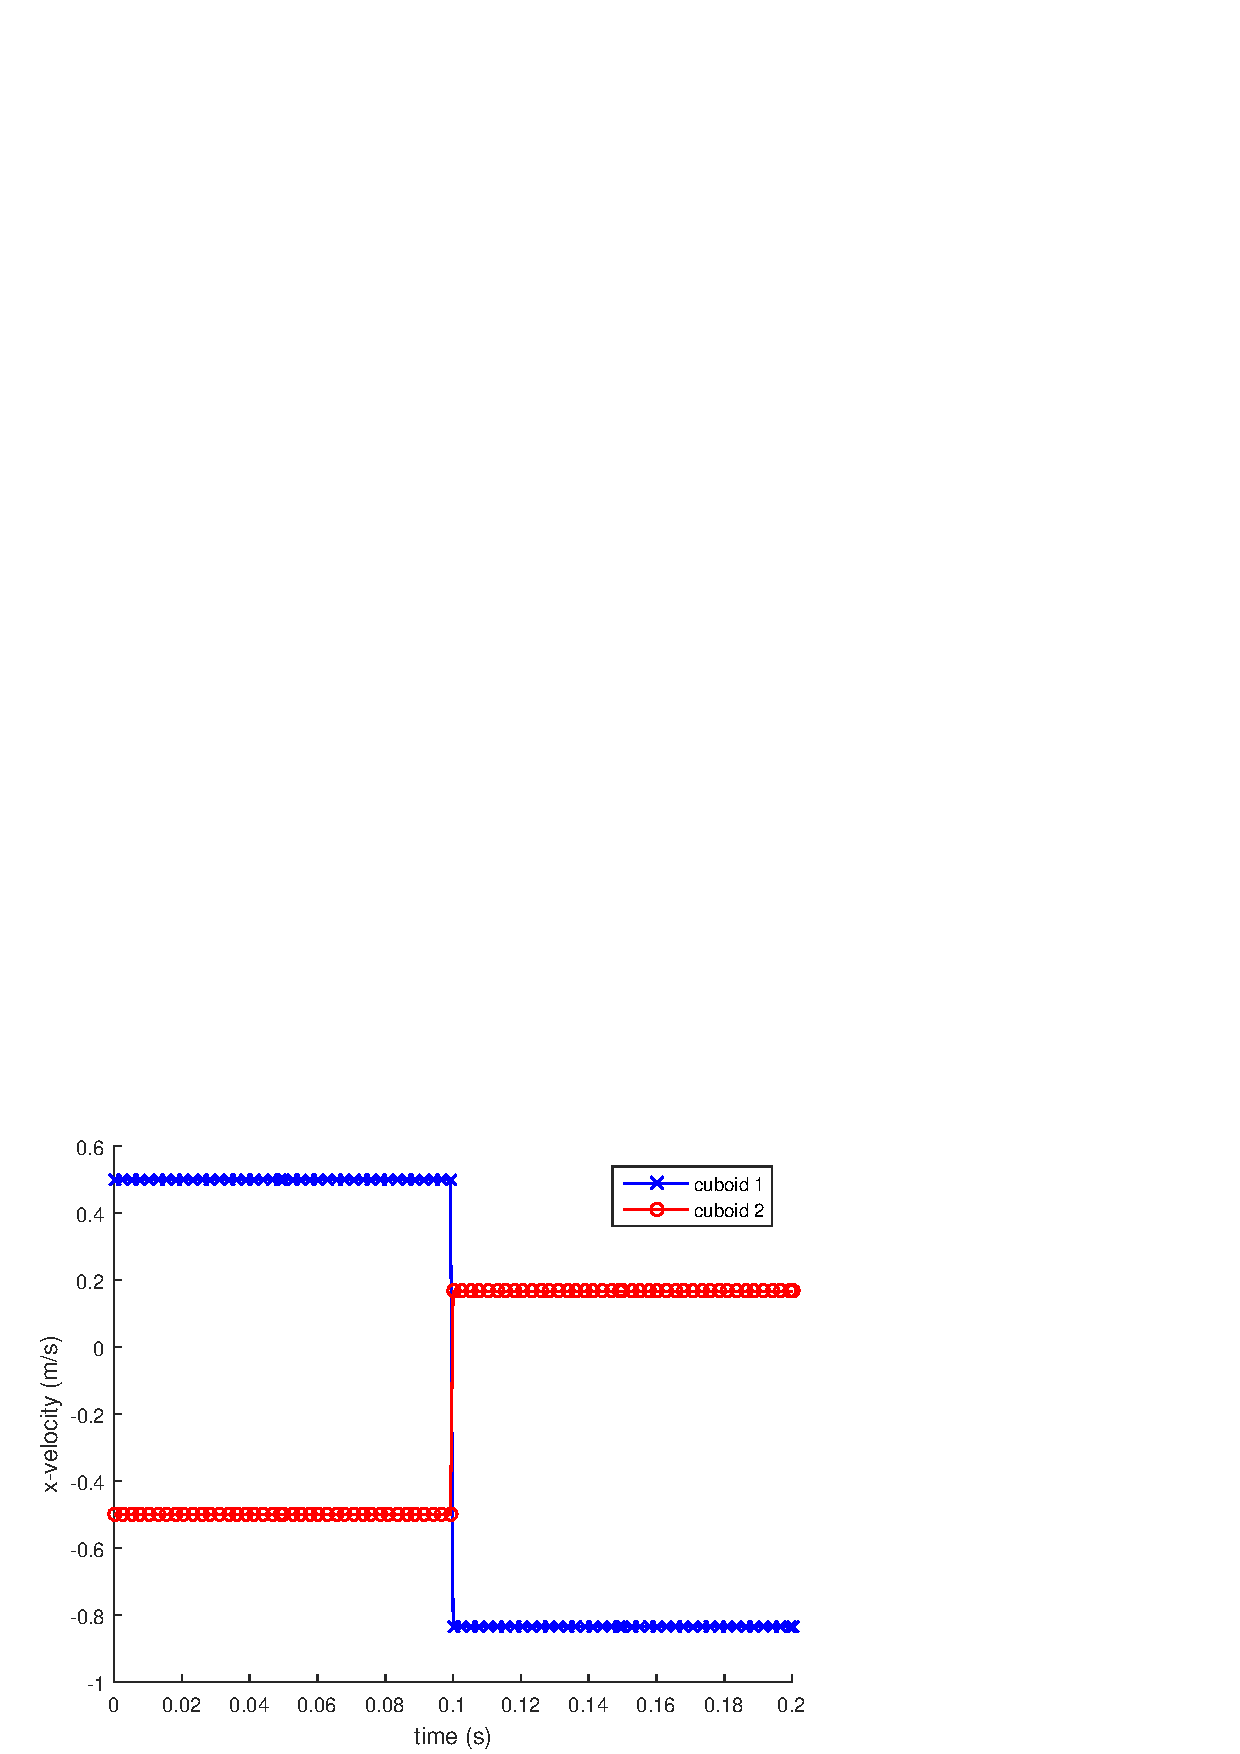
\includegraphics[width=0.48\textwidth]{figures/elastic}
\caption{The velocity profile of the two cuboids. The left figure is the
complete inelastic case ($C_R = 0$), and the right figure is the complete
elastic case ($C_R = 1$).}
\label{fig:rg_collsn_velo}
\end{figure}

\Fig{rg_collsn_velo} demonstrates the numerical profiles of
velocity in two extreme case: $C_R = 0$ and $C_R = 1$.
Clearly, it is consistent with the analytical values.
Taking complete inelastic case for example, three states of the process are
shown in \Fig{inelastic_collsn}.
\begin{figure}[!ht]
\centering
\includegraphics[width=0.32\textwidth]{figures/inelastic_0}
\includegraphics[width=0.32\textwidth]{figures/inelastic_1}
\includegraphics[width=0.32\textwidth]{figures/inelastic_2}
\caption{Complete inelastic collision. The left figure is the initial
state ($t = 0s$) and two cuboids are moving toward each other; the middle
figure is when they collide ($t = 0.1s$), after which both move to the left
with the same velocity; the right figure is the final state ($t = 1.0s$).}
\label{fig:inelastic_collsn}
\end{figure}

\subsection{Case 1: Cloth and Strings}
The first example involves the collision between elastic cloth and elastic
strings.
Initially, a flat circular cloth is right above a bunch of strings which are
straight and parallel, with their ends fixed.
Due to the gravity, cloth and strings fall and collide with each.
In this example, cloth-string collision happens first.
Then, when the cloth is folded, the strings are clustered and string-string
collision occurs.
Finally, two half parts of the cloth meet below the strings, self-collision
of cloth appears.
\Fig{fall_string} demonstrates this process, and we can observe,
all the three kinds of collision are handled properly.
\begin{figure}[!ht]
\centering
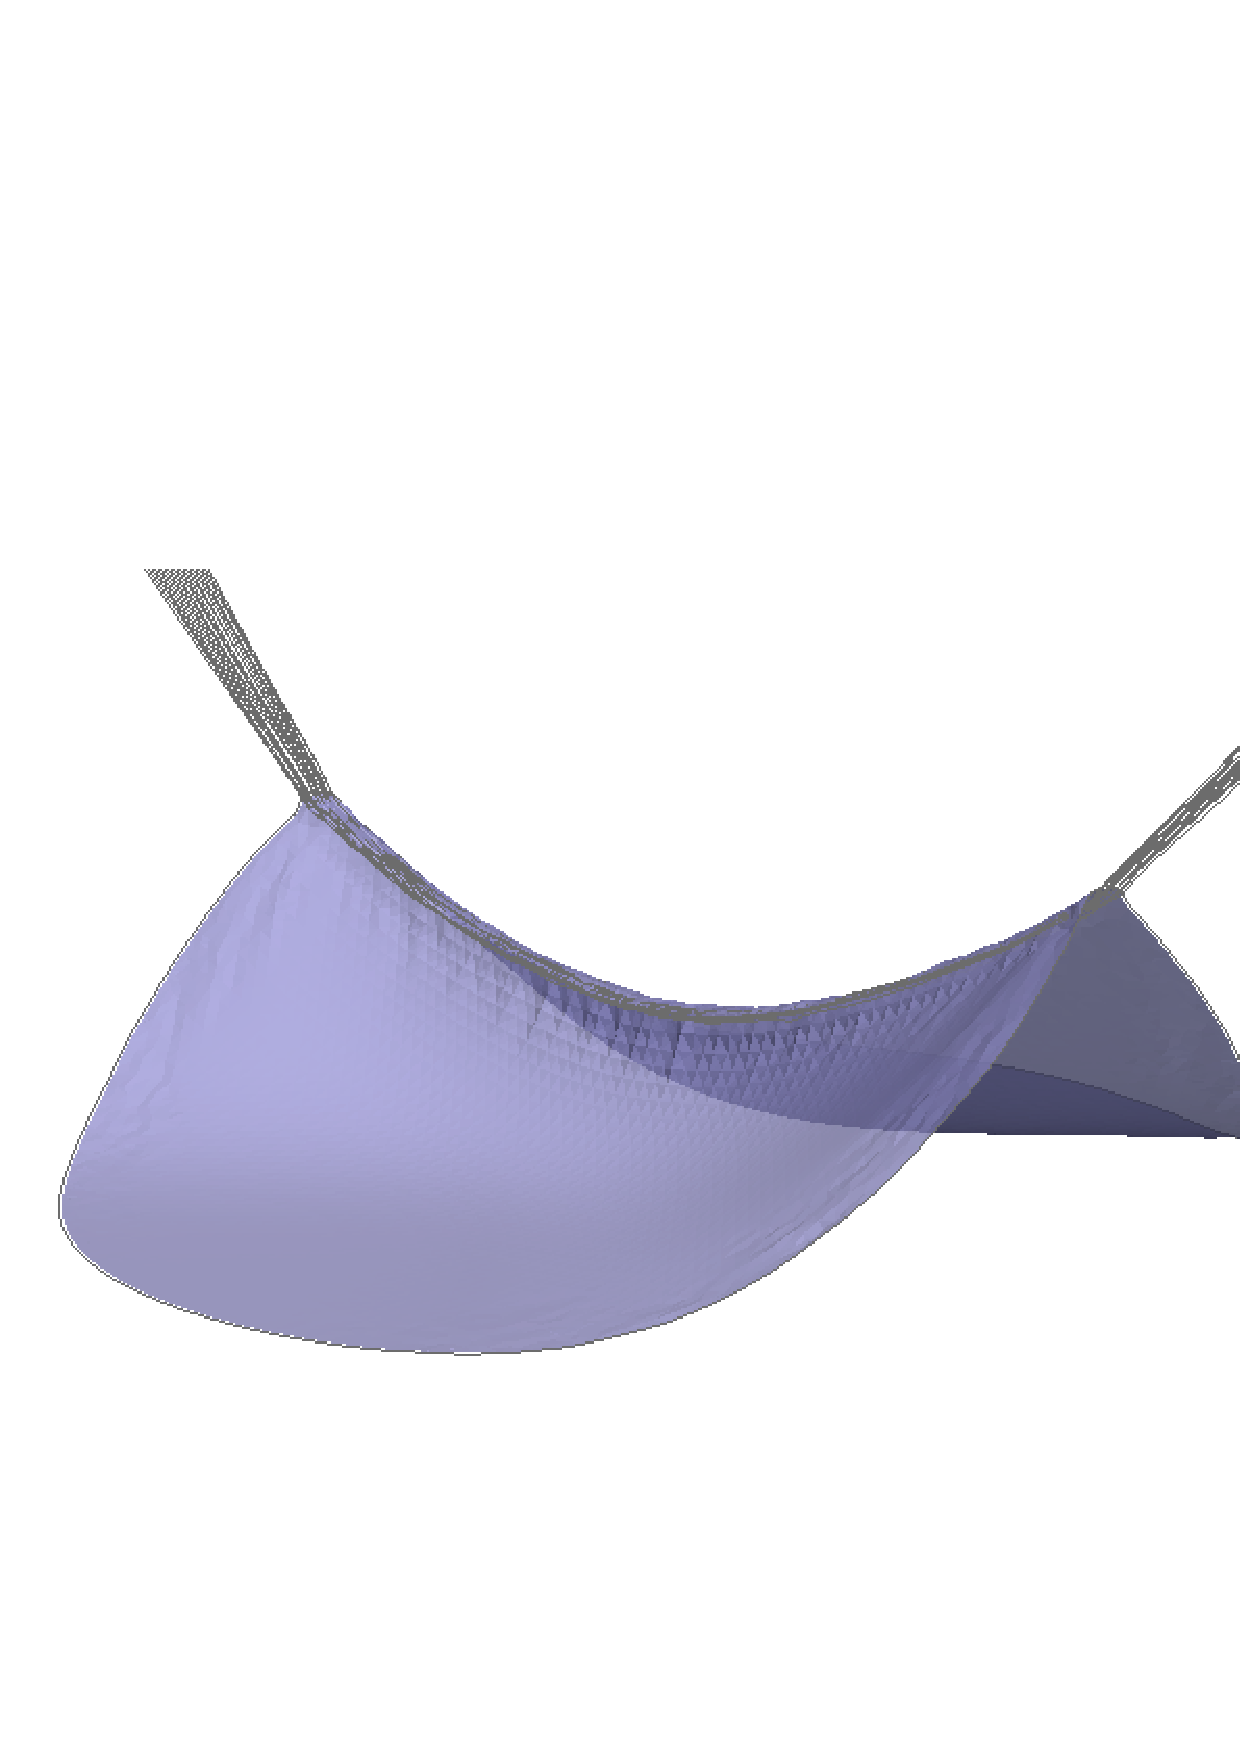
\includegraphics[width=0.48\textwidth]{figures/fall_string_0}
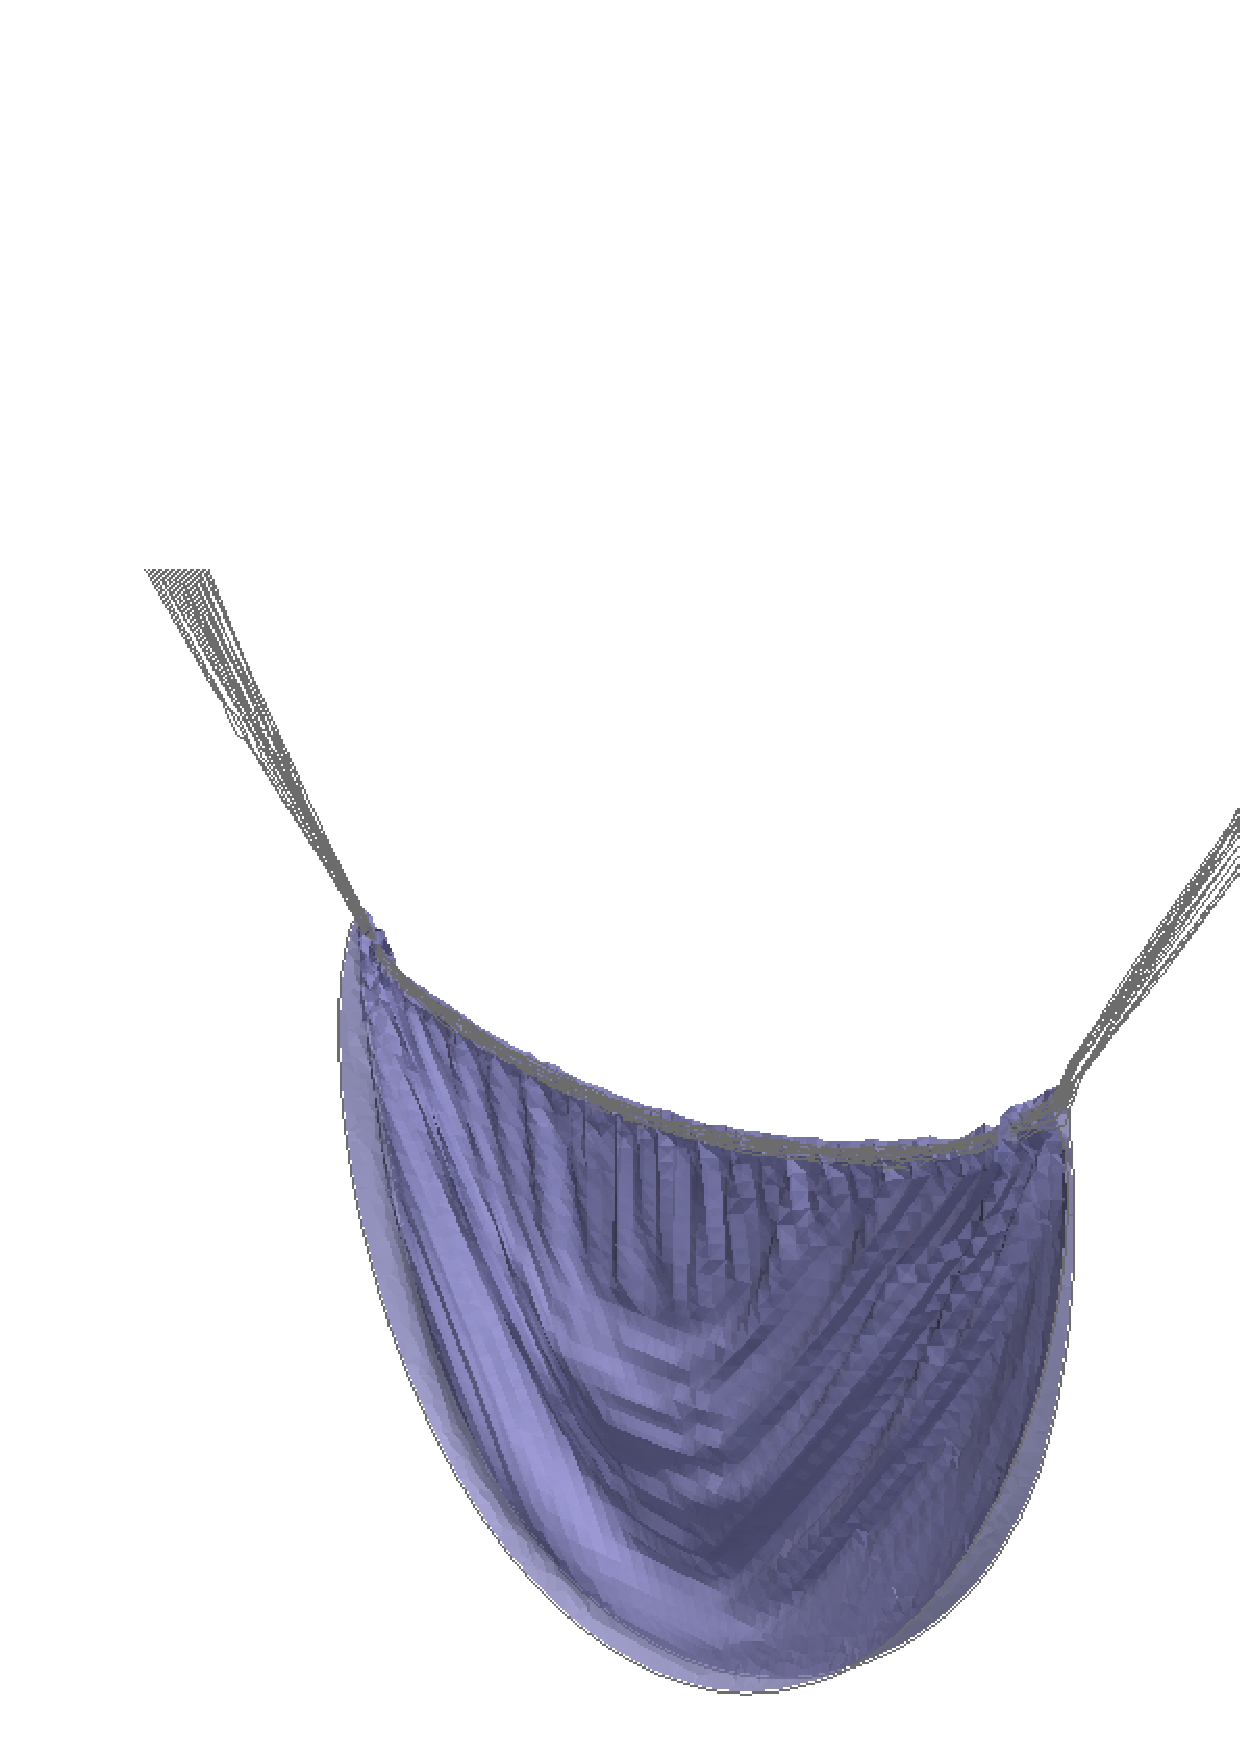
\includegraphics[width=0.48\textwidth]{figures/fall_string_1}
\caption{Two stages in the process of a circular cloth falling onto a
bunch of elastic strings. In the left figure, there are collisions between
cloth and strings. While in the right figure, the are also collisions
between the strings and self-collision of cloth.}
\label{fig:fall_string}
\end{figure}

\subsection{Case 2: Rigid Body and Cloth}
Here, we exhibit two examples demonstrating the collision between rigid
bodies and cloth.
In \Fig{rigid_cloth_collsn}, a circular fabric falls from some height
above the static cuboid object.
The bending force is taken into account in the way mentioned above. 
It highly reduces the number of collision pairs and forms the billows at
four corners.
\begin{figure}[!ht]
\centering
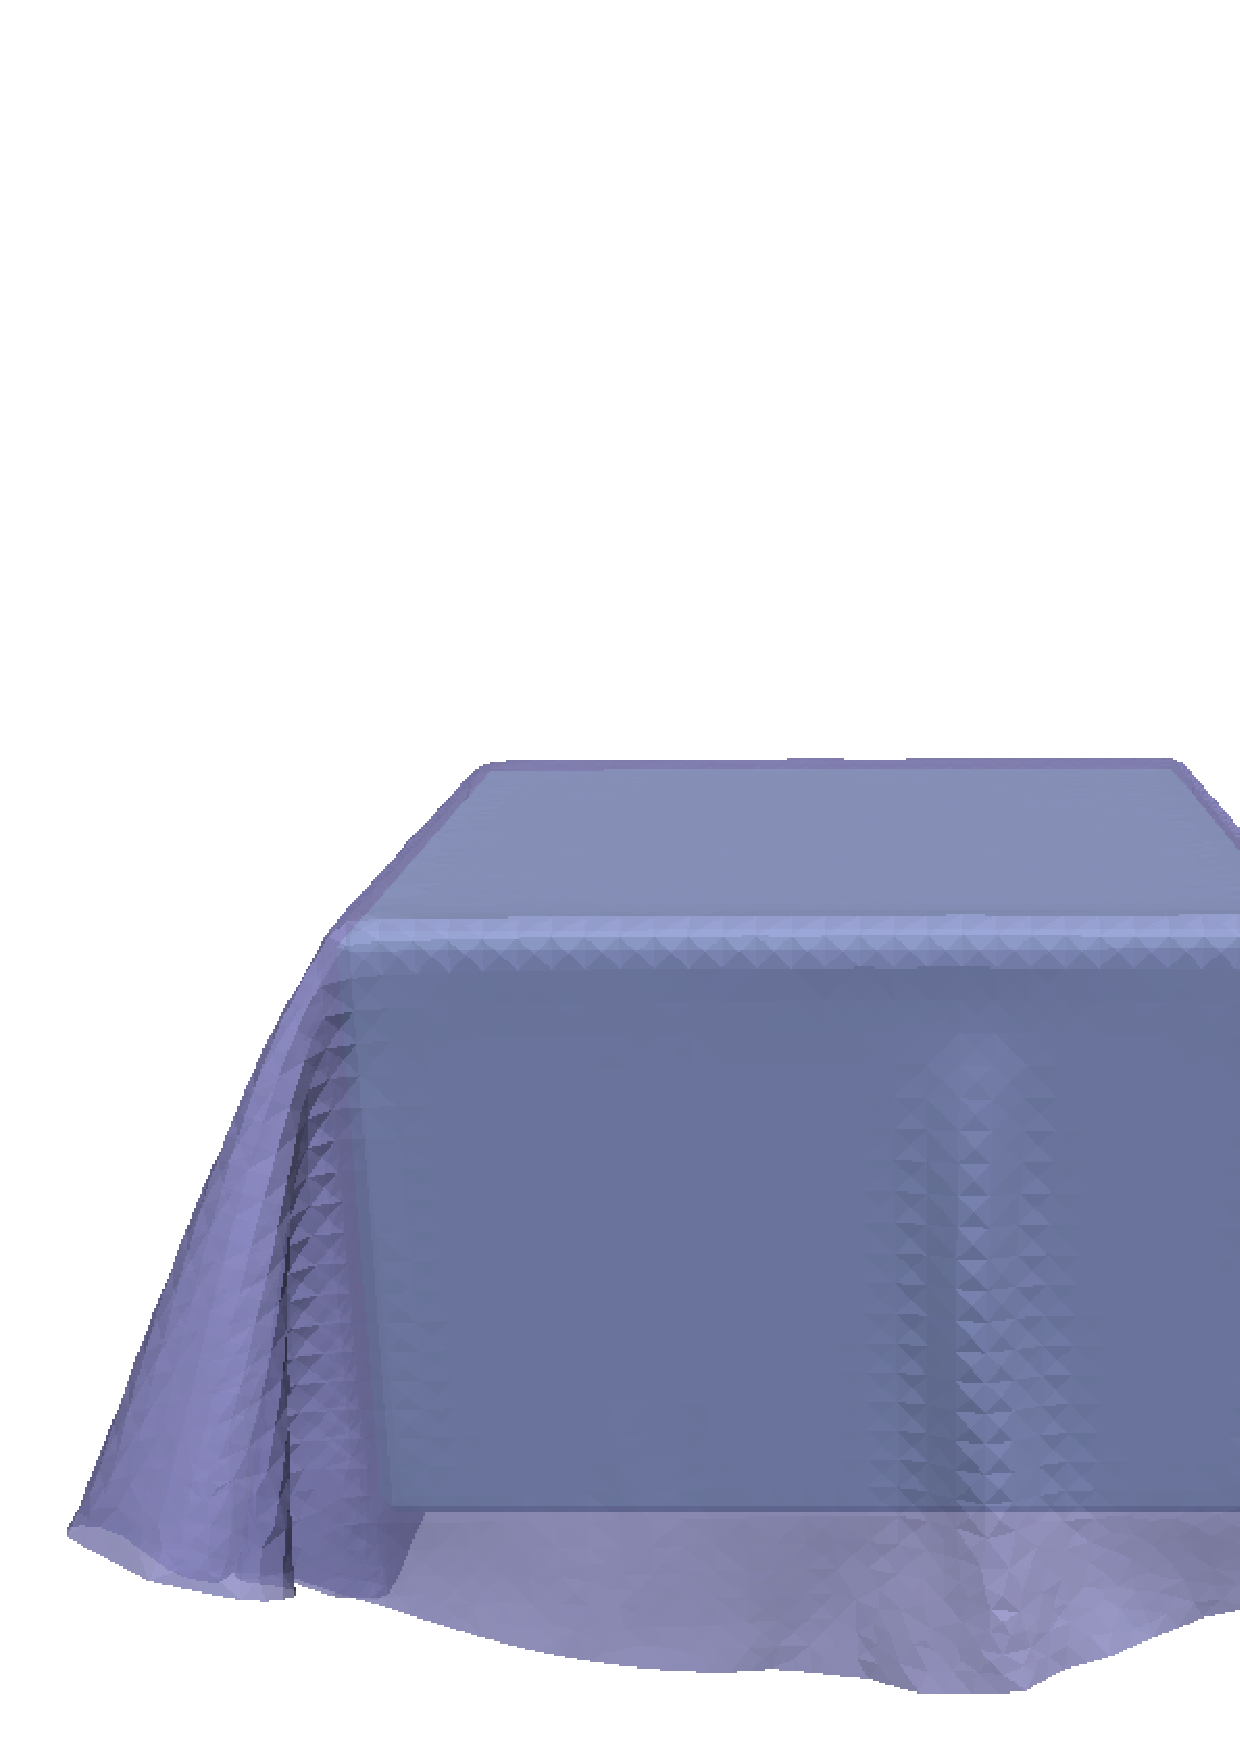
\includegraphics[width=0.48\textwidth]{figures/fall_box_0}
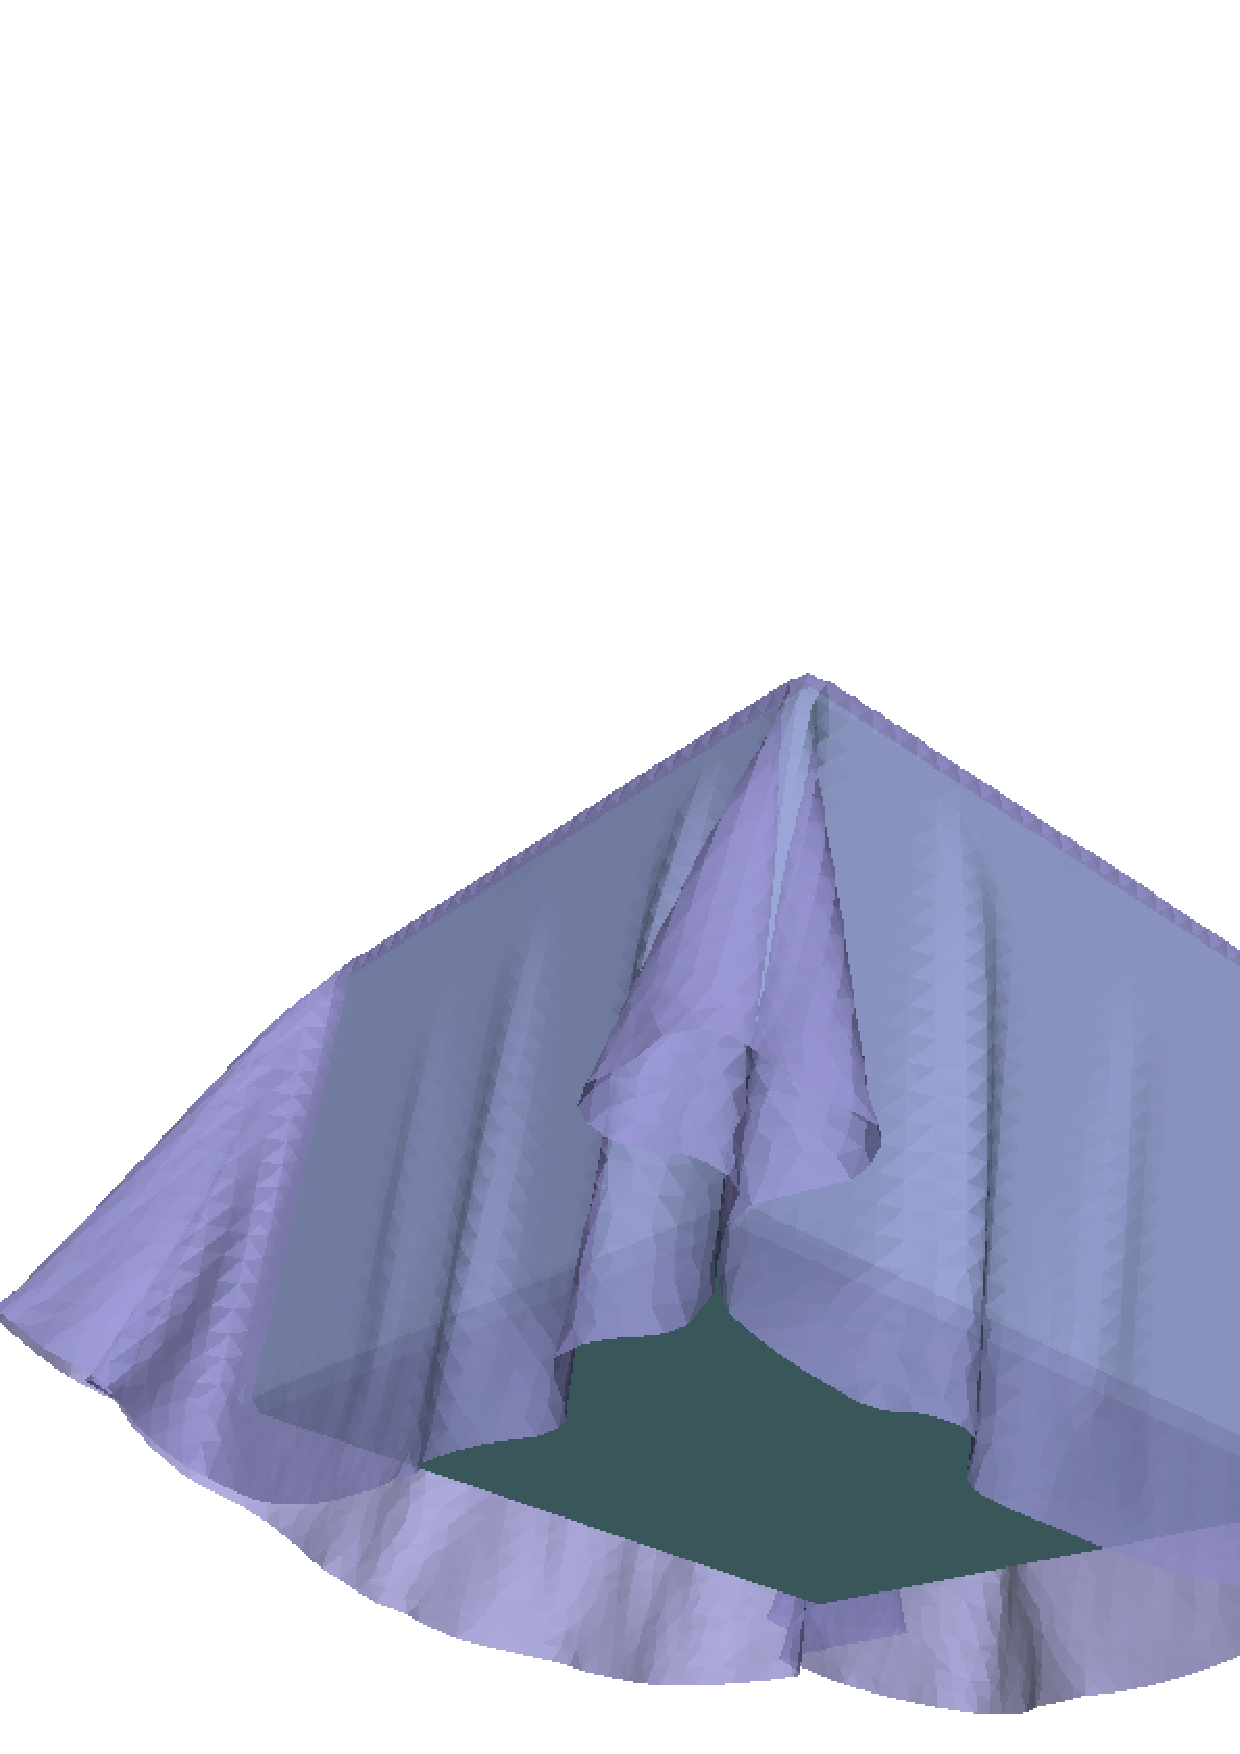
\includegraphics[width=0.48\textwidth]{figures/fall_box_1}
\caption{The front view and the side view of the cloth falling onto static
objects. Benefitted from the bending effect mentioned at the end of the
spring-mass model, billows appear at the courners.}
\label{fig:rigid_cloth_collsn}
\end{figure}

\Fig{2sphere_fall} is the falling process of two balls from some height
onto cloth with its left and right sides fixed.
In the early stage, two balls collide with the cloth, respectively, and
only rigid-elastic collision occurs.
Due to the bowl shape of the cloth, two balls are pushed towards each other
and collide at some time.
Since the collision between two balls is set to be completely inelastic,
they keep contacted and collide with the cloth together in the later stage.
\begin{figure}[!ht]
\centering
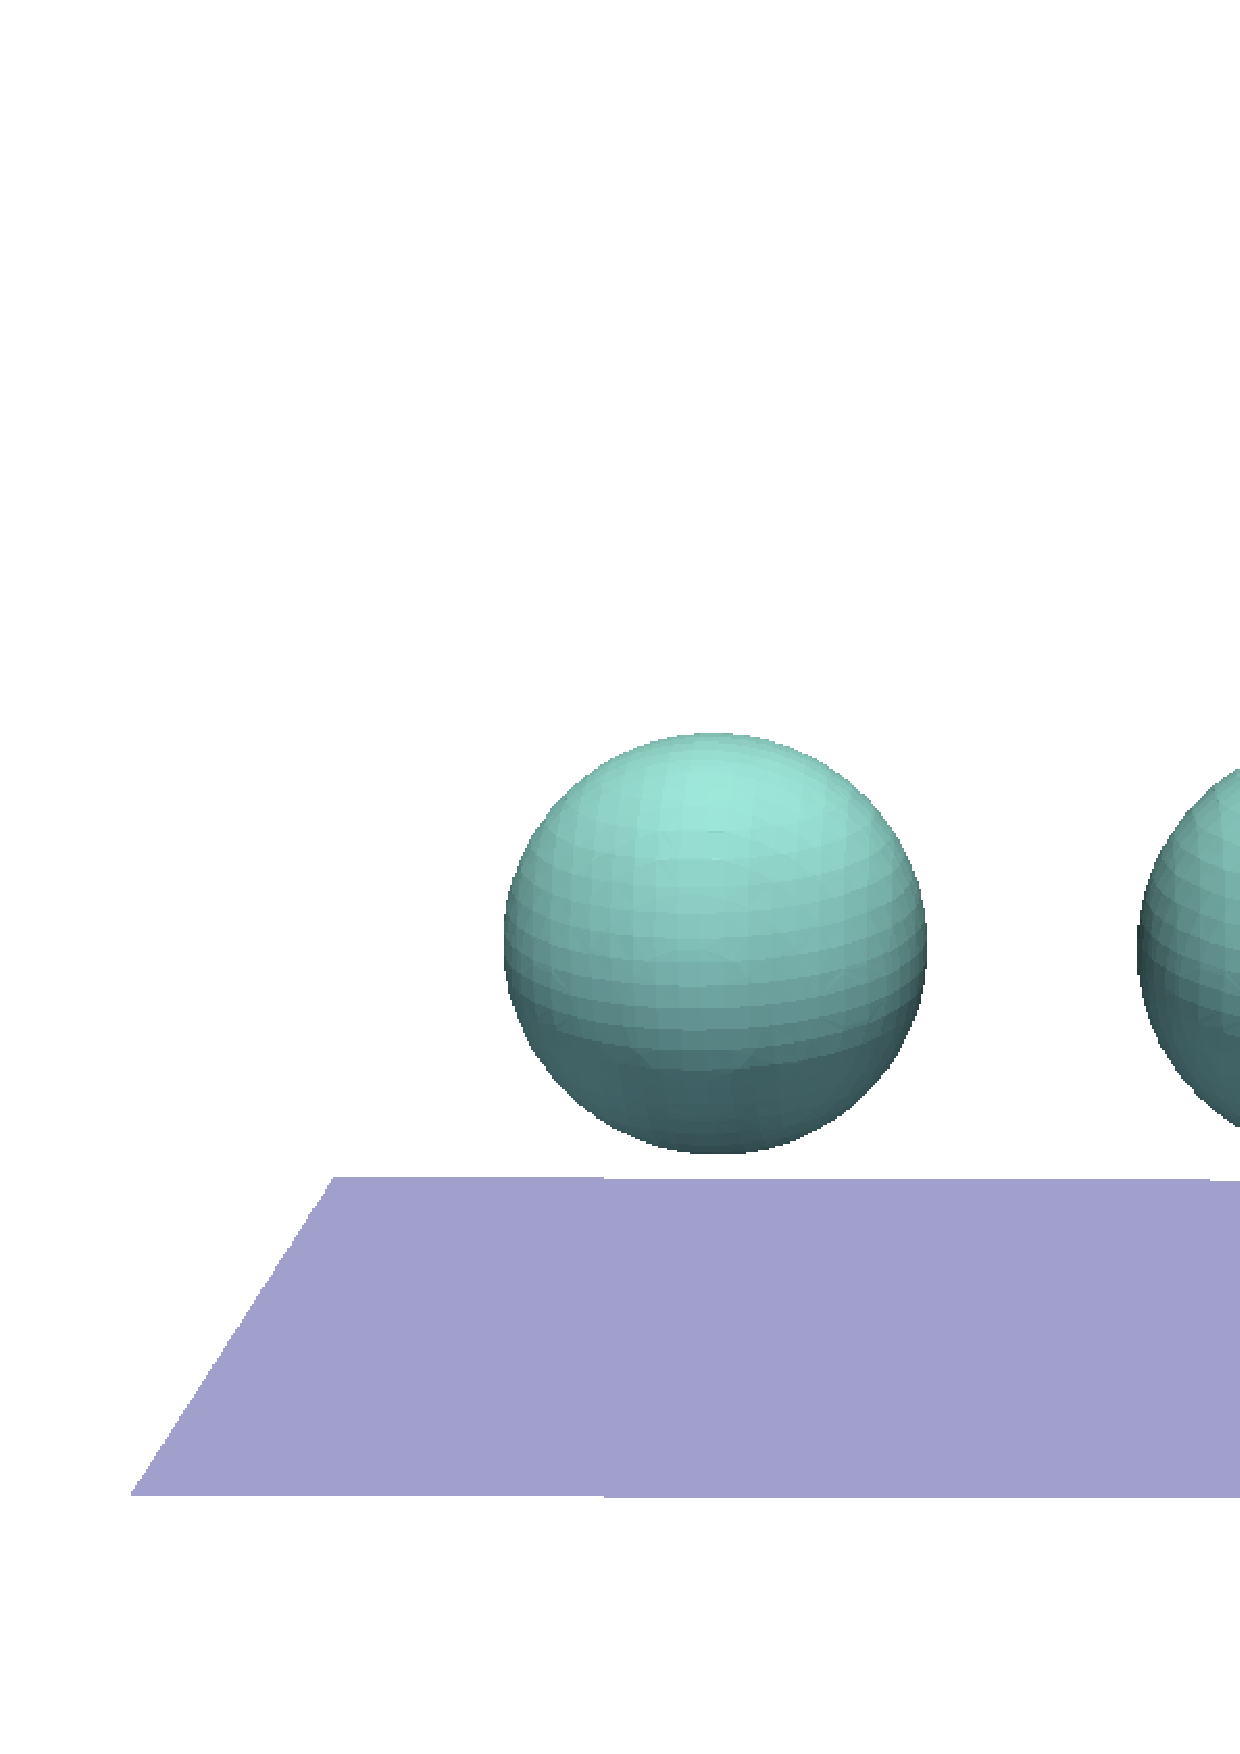
\includegraphics[width=0.48\textwidth]{figures/2sphere_fall_0}
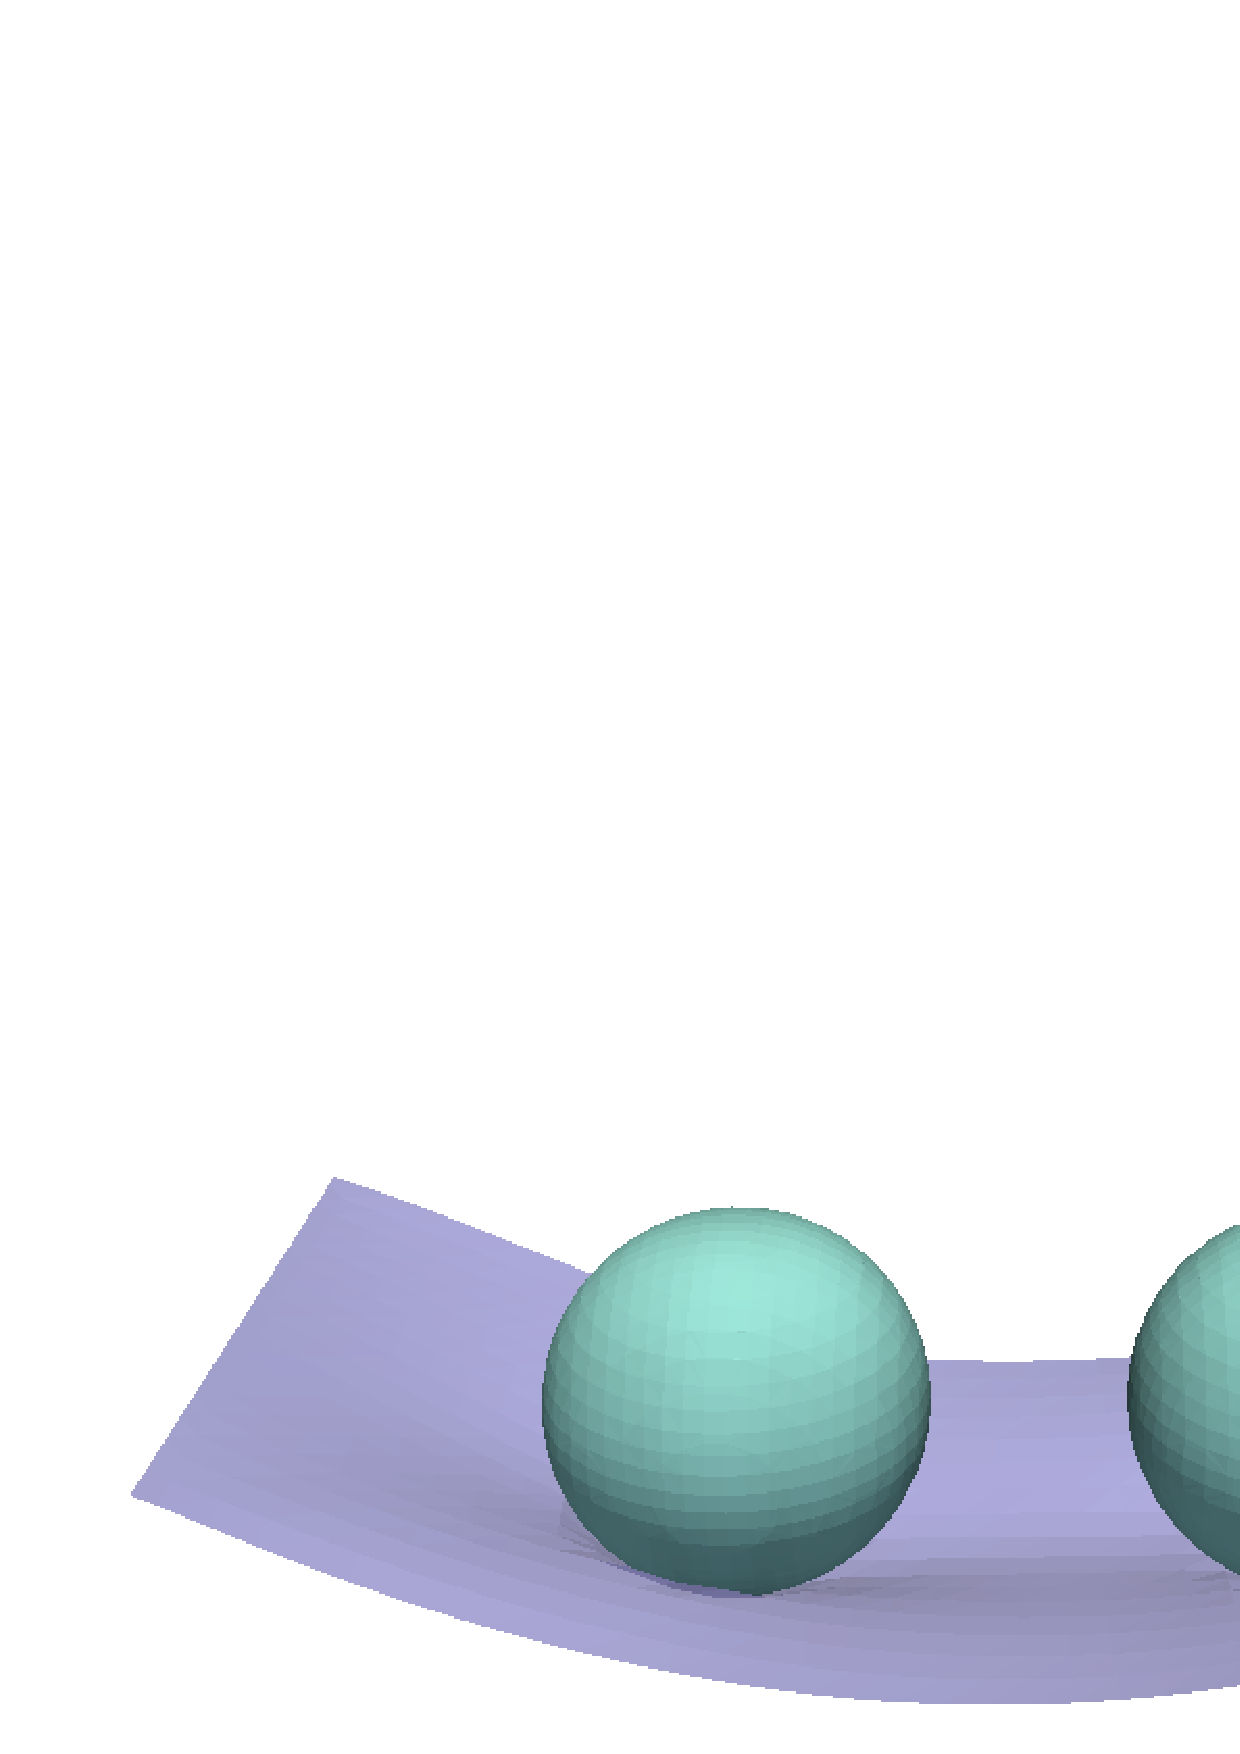
\includegraphics[width=0.48\textwidth]{figures/2sphere_fall_1} \\
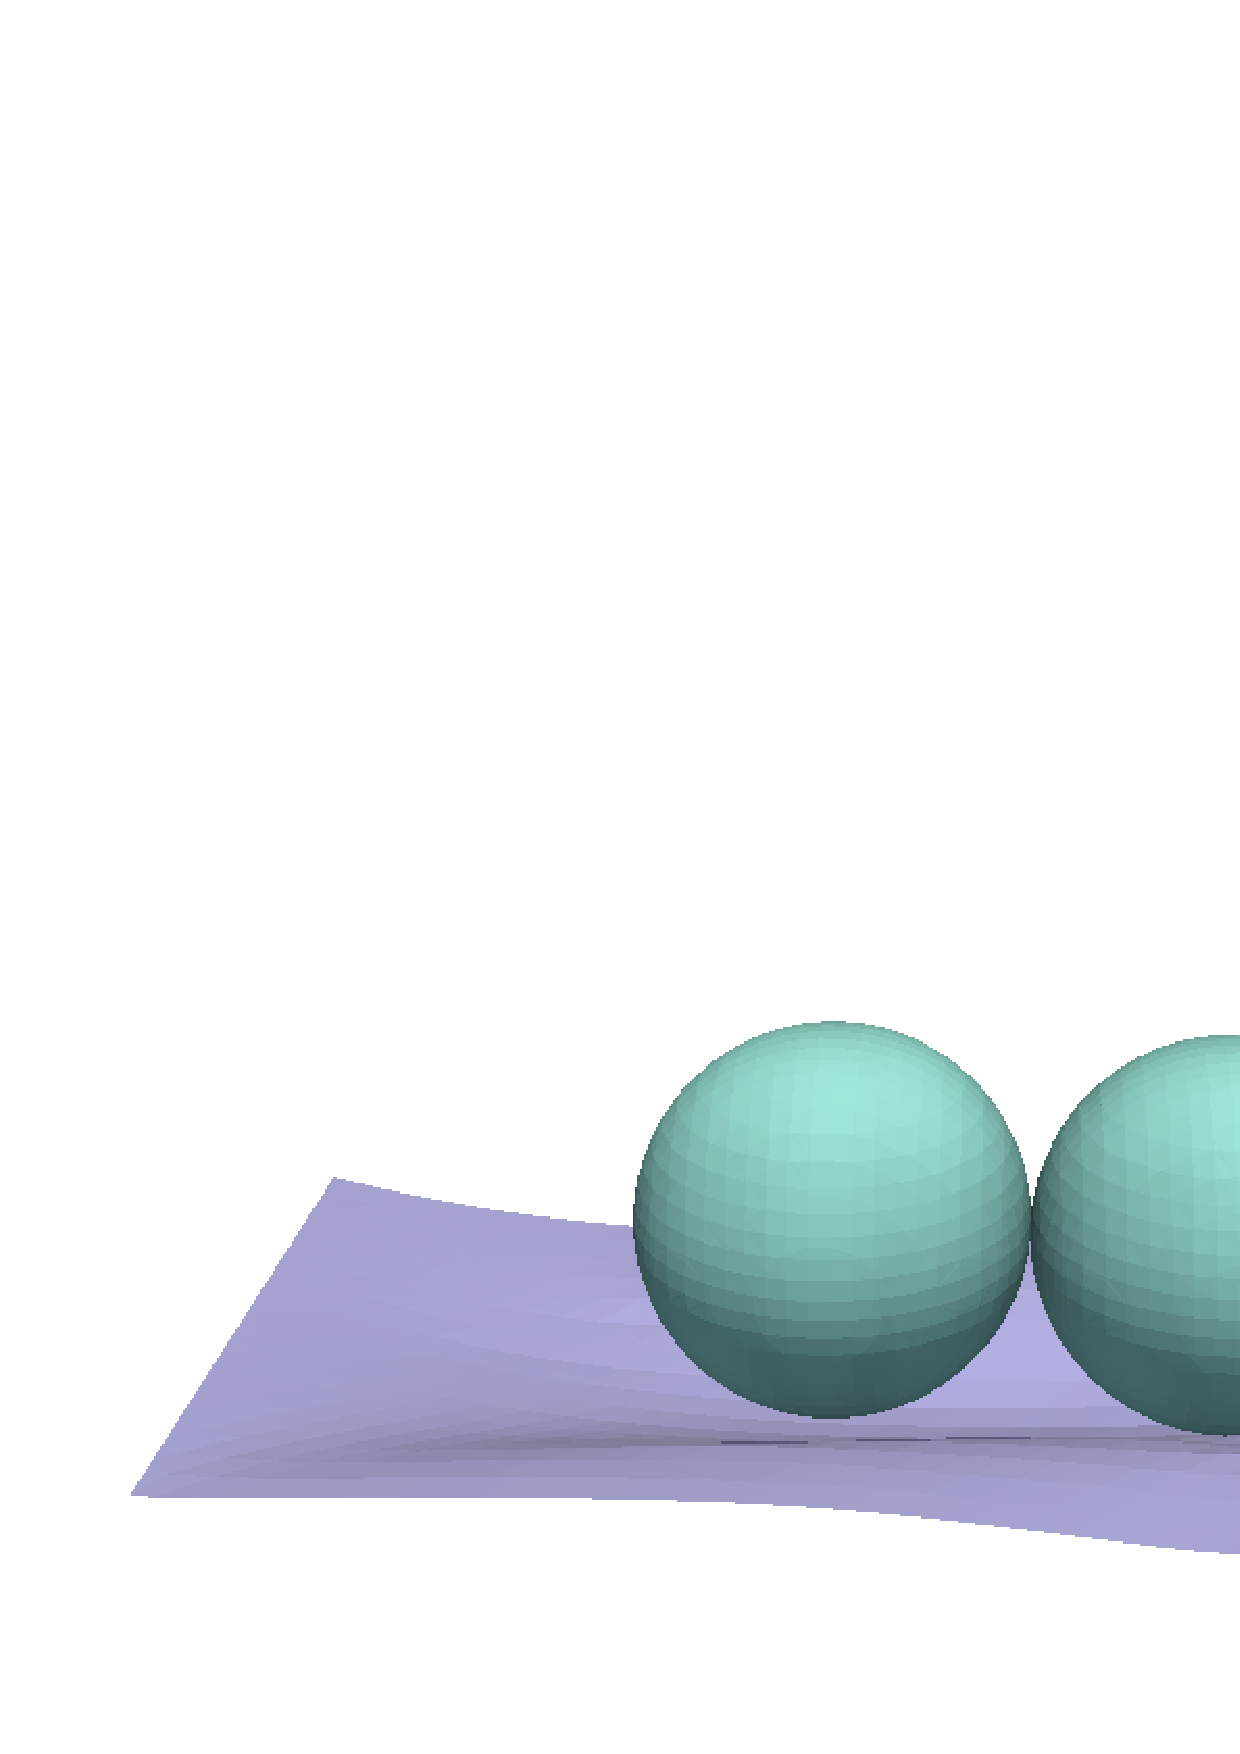
\includegraphics[width=0.48\textwidth]{figures/2sphere_fall_2}
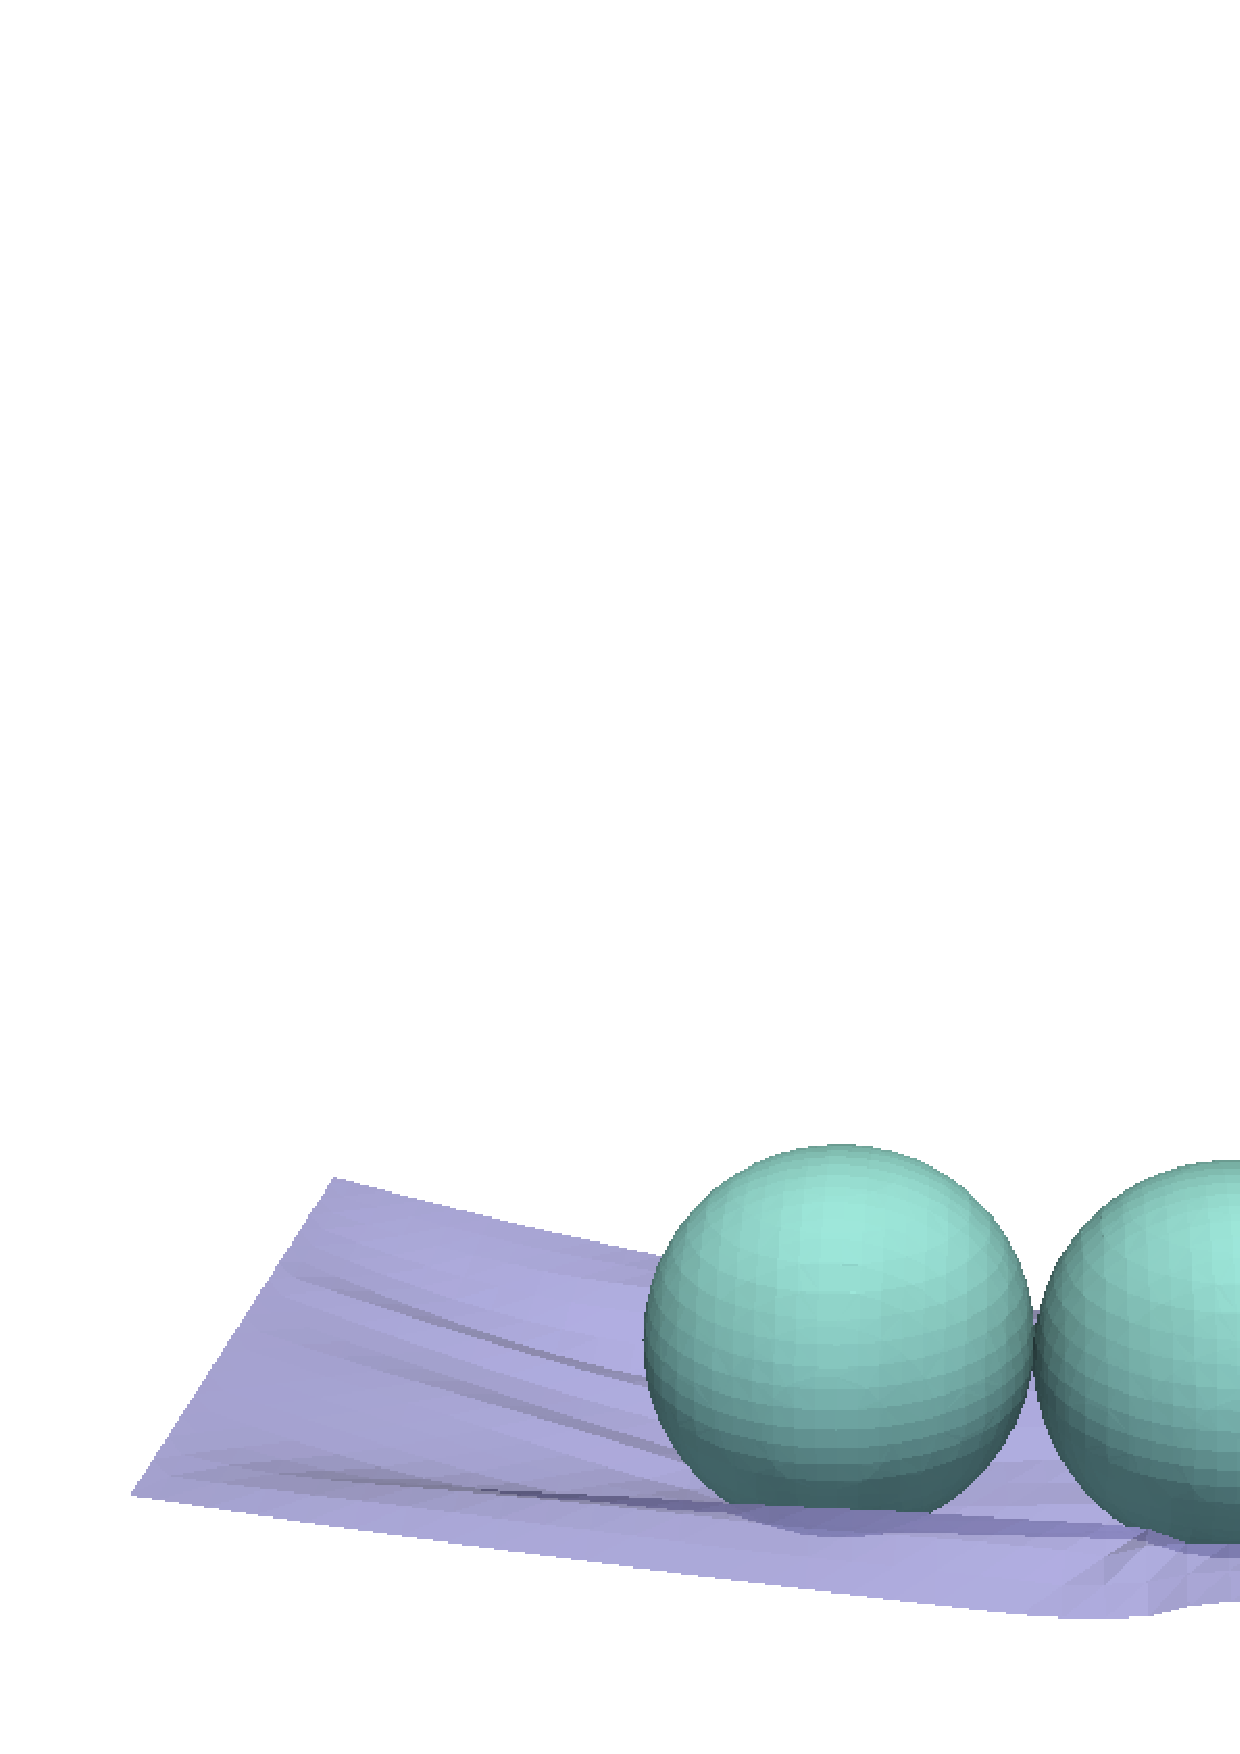
\includegraphics[width=0.48\textwidth]{figures/2sphere_fall_3}
\caption{Two balls falling on to cloth whose two sides are fixed. }
\label{fig:2sphere_fall}
\end{figure}



\newpage
 	   % Numerical Results
\chapter{General Network}
\label{chapter:concl}

\section{General Case With Front-end Processors}
\begin{equation}
{
\left[ \begin{array}{ccccccc}
1 & m_{1} & m_{2} & \cdots & m_{n-2} & m_{n-1} & m_{n}\\
1 & -1 & 0 & \cdots& 0 & 0 & 0\\
0 & \sigma -1 & 1 & \cdots & 0 & 0 & 0 \\
0 & \sigma -1 & \sigma & 1 & 0 & \cdots & 0 \\
0 & \sigma -1 & \sigma & \sigma & 1 & 0 & 0 \\
\vdots & \vdots & \vdots  &   \vdots & \ddots & \ddots\\
0 & \sigma -1 & \sigma & \cdots & \sigma & \sigma & 1
\end{array} 
\right ]} \times \left[ \begin{array}{c}
\alpha_{l_{0}} \\
\alpha_{l_{1}} \\
\alpha_{l_{2}} \\
\alpha_{l_{3}} \\
\vdots \\
\alpha_{l_{n-1}}\\
\alpha_{l_{n}}
\end{array} 
\right ] = \left[ \begin{array}{c}
1 \\
0 \\
0 \\
0 \\
\vdots \\
0
\end{array} 
\right ]
\end{equation}

The $m_{1}$, $m_{2}$, $\cdots$, $m_{n}$ are the number of processors on the $level_{1}$, $level_{2}$, $\cdots$, $level_{n}$.   Also, the $\alpha_{l0}$, $\alpha_{l1}$,  $\cdots$, $\alpha_{ln}$ are corresponding workload fraction.  

Finally, the speedup is:
$$Speedup = \frac{T_{f, 0}}{T_{f, n}}= \frac{\omega T_{cp}}{\alpha_{0}\omega T_{cp}} = \frac{1}{\alpha_{0}} = -\det A$$.
\newpage 


\section{General Case Without Front-end Processors}
\begin{equation}
{
\left[ \begin{array}{ccccccc}
1 & m_{1} & m_{2} & \cdots & m_{n-2} & m_{n-1} & m_{n}\\
1 & -(\sigma + 1) & 0 & \cdots& 0 & 0 & 0\\
1 & -\sigma & -(\sigma + 1) & \cdots & 0 & 0 & 0 \\
1 & -\sigma & -\sigma & -(\sigma + 1) & 0 & \cdots & 0 \\
1 & -\sigma & -\sigma & -\sigma & -(\sigma + 1) & 0 & 0 \\
\vdots & \vdots & \vdots  &   \vdots & \ddots & \ddots\\
1 & -\sigma & -\sigma & \cdots & -\sigma & -\sigma & -(\sigma + 1)
\end{array} 
\right ]} \times \left[ \begin{array}{c}
\alpha_{l_{0}} \\
\alpha_{l_{1}} \\
\alpha_{l_{2}} \\
\alpha_{l_{3}} \\
\vdots \\
\alpha_{l_{n-1}}\\
\alpha_{l_{n}}
\end{array} 
\right ] = \left[ \begin{array}{c}
1 \\
0 \\
0 \\
0 \\
\vdots \\
0
\end{array} 
\right ]
\end{equation}

The $m_{1}$, $m_{2}$, $\cdots$, $m_{n}$ are the number of processors on the $level_{1}$, $level_{2}$, $\cdots$, $level_{n}$.   Also, the $\alpha_{l0}$, $\alpha_{l1}$,  $\cdots$, $\alpha_{ln}$ are corresponding workload fraction. \\

The speedup is  
$$Speedup = \frac{T_{f, 0}}{T_{f, n}}= \frac{\omega T_{cp}}{\alpha_{0}\omega T_{cp}} = \frac{1}{\alpha_{0}} = \frac{\det A}{\det A^{\star}} = \left |\frac{\det A}{(\sigma^{\star})^{n-1}}\right|$$


	   % Parallelization
\chapter{Conclusions}
\label{chapter:concl}

\newpage
 	   % Conclusion
\end{spacing}

\begin{spacing}{\singlespace}	% Bibliographies must be
				% in single spacing in an entry and
				% double spacing between entries
				% MAKE SURE THE SPACING
\bibliographystyle{plain}	% plain or ieeetr

\bibliography{refs}
\end{spacing}

%\begin{spacing}{\defaultspace}  % adjust spacing
%\input{appendix}
%\end{spacing}

\end{document}
